% Arquivo LaTeX de exemplo de dissertação/tese a ser apresentada à CPG do IME-USP
%
% Criação: Jesús P. Mena-Chalco
% Revisão: Fabio Kon e Paulo Feofiloff
% Adaptação para UTF8, biblatex e outras melhorias: Nelson Lago
%
% Except where otherwise indicated, these files are distributed under
% the MIT Licence. The example text, which includes the tutorial and
% examples as well as the explanatory comments in the source, are
% available under the Creative Commons Attribution International
% Licence, v4.0 (CC-BY 4.0) - https://creativecommons.org/licenses/by/4.0/


%%%%%%%%%%%%%%%%%%%%%%%%%%%%%%%%%%%%%%%%%%%%%%%%%%%%%%%%%%%%%%%%%%%%%%%%%%%%%%%%
%%%%%%%%%%%%%%%%%%%%%%%%%%%%%%% PREÂMBULO LaTeX %%%%%%%%%%%%%%%%%%%%%%%%%%%%%%%%
%%%%%%%%%%%%%%%%%%%%%%%%%%%%%%%%%%%%%%%%%%%%%%%%%%%%%%%%%%%%%%%%%%%%%%%%%%%%%%%%

% "Book" tem capítulos (e partes, mas normalmente não usamos) e, se o documento
% é frente-e-verso, cada capítulo começa em uma página de numeração ímpar.
% Report é similar, mas cada capítulo começa em uma nova página, par ou ímpar.
% É possível mudar esse comportamento com a opção "openany". Observe que você
% pode adaptar este modelo para escrever artigos, mudando a classe do
% documento de "book" para "article" ou a classe de algum periódico específico.
%
% A opção frente-e-verso aqui significa, por exemplo, que as margens das páginas
% ímpares e pares são diferentes ou que números de página aparecem à direita
% ou à esquerda alternadamente. Nada impede que você crie um documento "só
% frente" e, ao imprimir, faça a impressão frente-e-verso.
%
% Aqui também definimos a língua padrão do documento e línguas adicionais. A
% classe em si não usa essa informação mas, passando as opções de língua aqui,
% elas são repassadas para todas as packages, e diversas packages mudam
% seu comportamento em função da língua (em especial, babel/polyglossia).
% A última língua da lista é a língua padrão do documento.
\documentclass[12pt,twoside,brazil,english]{book}
%\documentclass[12pt,twoside,english,brazil]{book}
%\documentclass[12pt,twoside,english,brazil]{article}

% tamanho da página e margens
\usepackage[a4paper]{geometry}
\geometry{
  % distância entre o início da página e o início do texto principal
  top=32mm,
  bottom=28mm,
  left=24mm,
  right=34mm,
  % Com geometry, esta medida não é tão relevante; basta garantir que ela
  % seja menor que "top" e que o texto do cabeçalho caiba nela.
  headheight=25.4mm,
  % distância entre o início do texto principal e a base do cabeçalho;
  % ou seja, o cabeçalho "invade" a margem superior nessa medida. Essa
  % é a medida que determina a posição do cabeçalho
  headsep=11mm,
  footskip=10mm,
  marginpar=20mm,
  marginparsep=5mm,
}

% Vários comandos auxiliares para o desenvolvimento de packages e classes;
% aqui, usamos em alguns comandos de formatação e condicionais.
\usepackage{etoolbox}
\usepackage{xstring}
\usepackage{xparse}

% Vários pacotes e opções de configuração genéricos; para personalizar o
% resultado, modifique estes arquivos.
%%%%%%%%%%%%%%%%%%%%%%%%%%%%%%%%%%%%%%%%%%%%%%%%%%%%%%%%%%%%%%%%%%%%%%%%%%%%%%%%
%%%%%%%%%%%%%%%%%%%%%%% CONFIGURAÇÕES E PACOTES BÁSICOS %%%%%%%%%%%%%%%%%%%%%%%%
%%%%%%%%%%%%%%%%%%%%%%%%%%%%%%%%%%%%%%%%%%%%%%%%%%%%%%%%%%%%%%%%%%%%%%%%%%%%%%%%

% Detecta o tipo de sistema que estamos usando (XeTeX, LuaTeX ou pdfTeX). Na
% verdade, ifpdf não detecta pdfTeX, mas sim se estamos gerando um PDF; como
% só XeTeX, LuaTeX e pdfTeX geram PDFs, combinando todos é possível identificar
% pdfTeX também.
\usepackage{ifxetex}
\usepackage{ifluatex}
\usepackage{ifpdf}

% "fontenc" é um parâmetro interno do LaTeX. O fontenc default é OT1, mas ele
% tem algumas limitações; a mais importante é que, com ele, palavras acentuadas
% não podem ser hifenizadas. Por conta disso, quase todos os documentos LaTeX
% utilizam o fontenc T1. A escolha do fontenc tem consequências para as fontes
% que podem ser usadas no documento; hoje em dia T1 tem mais opções de
% qualidade, então não se perde nada.
\usepackage[T1]{fontenc}

% apenas útil para LaTeX tradicional e pdfTeX; XeTeX e LuaTeX usam sempre utf8.
\usepackage[utf8]{inputenc}

% Permite criar "headed lists", ou seja, "listas" de elementos que vão
% aparecendo ao longo do documento (como, por exemplo, teoremas). Podem ser
% também citações a autores específicos, seções de um documento que está
% sendo analisado etc. Precisa ser carregado antes das definições de fontes.
\usepackage{amsthm}

% Internacionalização dos nomes das seções ("chapter" X "capítulo" etc.),
% hifenização e outras convenções tipográficas. babel deve ser um dos
% primeiros pacotes carregados. É possível passar a língua do documento
% como parâmetro aqui, mas já fizemos isso ao carregar a classe, no início
% do documento.
\usepackage{babel}

% É possível personalizar as palavras-chave que babel utiliza, por exemplo:
%\addto\extrasbrazil{\renewcommand{\chaptername}{Chap.}}
% Com BibTeX, isso vale também para a bibliografia; com BibLaTeX, é melhor
% usar o comando "DefineBibliographyStrings".

% Para línguas baseadas no alfabeto latino, como o inglês e o português,
% o pacote babel funciona muito bem, mas com outros alfabetos ele às vezes
% falha. Por conta disso, o pacote polyglossia foi criado para substituí-lo.
% polyglossia só funciona com LuaTeX e XeTeX; como babel também funciona com
% esses sistemas, provavelmente não há razão para usar polyglossia, mas é
% possível que no futuro esse pacote se torne o padrão.
%\usepackage{polyglossia}
%\setdefaultlanguage{brazil}
%\setotherlanguage{english}

% Alguns pacotes (espeficicamente, tikz) usam, além de babel, este pacote
% como auxiliar para a tradução de palavras-chave, como os meses do ano.
\usepackage{translator}

% microajustes no tamanho das letras, espaçamento etc. para melhorar
% a qualidade visual do resultado. LaTeX tradicional não dá suporte a
% nenhum tipo de microajuste; pdfLaTeX dá suporte a todos. LuaLaTeX
% e XeLaTeX dão suporte a alguns:
%
% * expansion não funciona com XeLaTeX
% * tracking não funciona com XeLaTeX; é possível obter o mesmo resultado
%   com a opção "LetterSpace" do pacote fontspec, mas a configuração é
%   totalmente manual. Por padrão, aumenta o afastamento entre caracteres
%   nas fontes "small caps"; o resultado não se presta ao uso na
%   bibliografia ou citações, então melhor desabilitar.
% * kerning e spacing só funcionam com pdfLaTex; ambas são funções
%   consideradas experimentais e nem sempre produzem resultados vantajosos.

\newcommand\microtypeopts{
  protrusion=true,
  tracking=false,
  kerning=false,
  spacing=false
}

\ifxetex
  \usepackage[expansion=false,\microtypeopts]{microtype}
\else
  \usepackage[expansion=true,\microtypeopts]{microtype}
\fi

% Alguns "truques" (sujos?) para minimizar over/underfull boxes.
%
% Para fazer um texto justificado, é preciso modificar o tamanho dos espaços
% em cada linha para mais ou para menos em relação ao seu tamanho ideal. Para
% escolher as quebras de linha, TeX vai percorrendo o texto procurando lugares
% possíveis para quebrar as linhas considerando essa flexibilidade mas dentro
% de um certo limite mínimo/máximo. Nesse processo, ele associa a cada possível
% linha o valor badness, que é o nível de distorção do tamanho dos espaços
% daquela linha em relação ao ideal, e ignora opções que tenham badness muito
% grande (esse limite é dado por \tolerance). Depois de encontradas todas as
% possíveis quebras de linha e a badness de cada uma, TeX calcula as penalties
% e demerits de cada possibilidade e escolhe a solução que minimiza o demerit
% total do parágrafo.
%
% Para cada fonte, o espaço em TeX tem um tamanho ideal, um tamanho mínimo e um
% tamanho máximo. TeX nunca reduz um espaço para menos que o mínimo da fonte,
% mas pode aumentá-lo para mais que o máximo. Se os espaços de uma linha ficam
% com o tamanho ideal, a badness da linha é 0; se o tamanho é
% reduzido/aumentado 50% do mínimo/máximo, a badness da linha é 12; se o
% tamanho é reduzido/aumentado para o mínimo/máximo, a badness é 100. Se esse
% aumento for de 30% além do máximo, a badness da linha é 200; se for de 45%
% além do máximo, a badness é 300; se for de 60% além do máximo, a badness é
% 400; se for de 100% além do máximo, a badness é 800.
%
% A \tolerance default é 200; aumentar para, digamos, 300 ou 400, permite que
% TeX escolha parágrafos com maior variação no espaçamento. No entanto, no
% cálculo de demerits, a badness de cada linha é elevada ao quadrado, então TeX
% geralmente prefere escolher outras opções no lugar de uma linha ruim. Por
% exemplo, órfãs/viúvas têm demerit de 22.500 e dois hífens seguidos têm
% demerit de 10.000 e, portanto, não é surpreendente que a maioria dos
% parágrafos tenha demerits abaixo de 40.000, quase todos abaixo de 100.000 e
% praticamente nenhum acima de 1.000.000. Isso significa que, para a grande
% maioria dos parágrafos, aumentar \tolerance não faz diferença: uma linha com
% badness 400 (correspondendo a demerit de 160.000) nunca será efetivamente
% escolhida se houver qualquer outra opção com badness menor. Também fica claro
% que não há muita diferença real entre definir \tolerance como 800 ou 9.999.
%
% O problema muda de figura se TeX não consegue encontrar uma solução. Isso
% pode acontecer em dois casos: (1) o parágrafo tem ao menos uma linha que não
% pode ser quebrada com badness < 10.000 e (2) o parágrafo tem ao menos uma
% linha que não pode ser quebrada com badness < tolerance (mas essa badness é
% menor que 10.000).
%
% No primeiro caso, se houver várias possibilidades de linhas que não podem ser
% quebradas, TeX não vai ser capaz de compará-las e escolher a melhor: todas
% têm a badness máxima (10.000) e, portanto, a que gerar menos deméritos no
% restante do parágrafo será a escolhida. Na realidade, no entanto, essas
% linhas *não* são igualmente ruins entre si, o que pode levar TeX a fazer uma
% má escolha. Para evitar isso, TeX tenta novamente aplicando
% \emergencystretch, que "faz de conta" que o tamanho máximo ideal dos espaços
% da linha é maior que o definido na fonte. Isso reduz a badness de todas as
% linhas, o que soa parecido com aumentar \tolerance. Há três diferenças, no
% entanto: (1) essa mudança só afeta os parágrafos que falharam; (2) soluções
% que originalmente teriam badness = 10.000 (e, portanto, seriam vistas como
% equivalentes) podem ser avaliadas e comparadas entre si; e (3) como a badness
% de todas as linhas diminui, a possibilidade de outras linhas que
% originalmente tinham badness alta serem escolhidas aumenta. Esse último ponto
% significa que \emergencystretch pode fazer TeX escolher linhas mais
% espaçadas, fazendo o espaçamento do parágrafo inteiro aumentar e, portanto,
% tornando o resultado mais homogêneo mesmo com uma linha particularmente ruim.
%
% É esse último ponto que justifica o uso de \emergencystretch no segundo caso
% também: apenas aumentar a tolerância, nesse caso, poderia levar TeX a
% diagramar uma linha ruim em meio a um parágrafo bom, enquanto
% \emergencystretch pode fazer TeX aumentar o espaçamento de maneira geral no
% parágrafo, minimizando o contraste da linha problemática com as demais.
% Colocando a questão de outra maneira, aumentar \tolerance para lidar com
% esses parágrafos problemáticos pode fazê-los ter uma linha especialmente
% ruim, enquanto \emergencystretch pode dividir o erro entre várias linhas.
% Assim, definir \tolerance em torno de 800 parece razoável: no caso geral,
% não há diferença e, se um desses casos difíceis não pode ser resolvido com
% uma linha de badness até 800, \emergencystretch deve ser capaz de gerar um
% resultado igual ou melhor.
%
% Penalties & demerits: https://tex.stackexchange.com/a/51264
% Definições (fussy, sloppy etc.): https://tex.stackexchange.com/a/241355
% Mais definições (hfuzz, hbadness etc.): https://tex.stackexchange.com/a/50850
% Donald Arseneau defendendo o uso de \sloppy: https://groups.google.com/d/msg/comp.text.tex/Dhf0xxuQ66E/QTZ7aLYrdQUJ
% Artigo detalhado sobre \emergencystretch: https://www.tug.org/TUGboat/tb38-1/tb118wermuth.pdf
% Esse artigo me leva a crer que algo em torno de 1.5em é suficiente

\tolerance=800
\hyphenpenalty=100 % Default 50; se o texto é em 2 colunas, 50 é melhor
\setlength{\emergencystretch}{2.5em}

% Não gera warnings para Overfull menor que 0.5pt
\hfuzz=.5pt
\vfuzz\hfuzz

% Não gera warnings para Underfull com badness < 1000
\hbadness=1000
\vbadness=1000

% LaTeX às vezes coloca notas de rodapé logo após o final do texto da
% página ao invés de no final da página; este pacote evita isso.
\usepackage[bottom]{footmisc}

% Se uma página está vazia, não imprime número de página ou cabeçalho
\usepackage{emptypage}

% Espaçamento entre linhas configurável (\singlespacing, \onehalfspacing etc.)
\usepackage{setspace}

% Carrega nomes de cores disponíveis (podem ser usados com hyperref e listings)
\usepackage[usenames,svgnames,dvipsnames]{xcolor}

% LaTeX define os comandos "MakeUppercase" e "MakeLowercase", mas eles têm
% algumas limitações; esta package define os comandos MakeTextUppercase e
% MakeTextLowercase que resolvem isso.
\usepackage{textcase}

% Normalmente, LaTeX faz o final da página terminar sempre no mesmo lugar
% (exceto no final dos capítulos). Esse padrão pode ser ativado explicitamente
% com o comando "\flushbottom". Mas se, por alguma razão, o volume de texto na
% página é "pequeno", essa página vai ter espaços verticais artificialmente
% grandes. Uma solução para esse problema é modificar o padrão para
% "\raggedbottom"; isso permite que as páginas terminem em lugares diferentes.
% Outra opção é corrigir manualmente cada página problemática, por exemplo
% com o comando "\enlargethispage".
%\raggedbottom

% Por padrão, LaTeX coloca uma espaço aumentado após sinais de pontuação;
% Isso não é tão bom quanto alguns TeX-eiros defendem :) .
% Esta opção desabilita isso e, consequentemente, evita problemas com
% "id est" (i.e.) e "exempli gratia" (e.g.)
\frenchspacing

% Tanto Small Caps quanto itálico (ou slanted) são "shapes" de uma fonte.
% Sendo assim, os comandos \scshape (ou \textsc) e \itshape (ou \textit) são
% "incompatíveis" entre si, ou seja, um cancela o outro. O que LaTeX faz é
% considerar que há um outro shape: "small caps + itálico" (ou "small caps +
% slanted"), chamado "scit" ou "scsl". Se a fonte oferece esse shape, é só
% usar \fontshape(scit}\selectfont. Mas isso é muito desconfortável, já que
% o usual seria algo como "\textsc{Algumas \textit{palavras} podem ser
% diferentes}". Esta package resolve esse problema.
\usepackage{slantsc}

% LaTeX procura por arquivos adicionais no diretório atual e nos diretórios
% padrão do sistema. Assim, é preciso usar caminhos relativos para incluir
% arquivos de subdiretórios: "\input{diretorio/arquivo}". No entanto, há
% duas limitações:
%
% 1. É necessário dizer "\input{diretorio/arquivo} mesmo quando o arquivo
%    que contém esse comando já está dentro do subdiretório.
%
% 2. Isso não deve ser usado para packages ("\usepackage{diretorio/package}"),
%    embora na prática funcione.
%
% O modo recomendado de resolver esses problemas é modificando o arquivo
% texmf.cnf ou a variável de ambiente TEXINPUTS ou colocando os arquivos
% compartilhados na árvore TEXMF (geralmente, no diretório texmf dentro do
% diretório do usuário), o que é um tanto complicado para usuários menos
% experientes.
%
% O primeiro problema pode ser solucionado também com a package import,
% mas não há muita vantagem pois é preciso usar outro comando no lugar de
% "\input". O segundo problema é mais importante, pois torna muito difícil
% colocar packages adicionais em um diretório separado. Para contorná-lo,
% vamos usar um truque que é suficiente para nossa necessidade, embora
% *não* seja normalmente recomendado.
%\usepackage{import}

\newcommand\usepackagefromsubdir[3][]{
    \csletcs{@oldinput@path}{input@path}
    \csappto{input@path}{{#2}}
    \usepackage[#1]{#3}
    \csletcs{input@path}{@oldinput@path}
}

\newcommand\usethemefromsubdir[3][]{
    \csletcs{@oldinput@path}{input@path}
    \csappto{input@path}{{#2}}
    \usetheme[#1]{#3}
    \csletcs{input@path}{@oldinput@path}
}

\newcommand\usecolorthemefromsubdir[3][]{
    \csletcs{@oldinput@path}{input@path}
    \csappto{input@path}{{#2}}
    \usecolortheme[#1]{#3}
    \csletcs{input@path}{@oldinput@path}
}

%%%%%%%%%%%%%%%%%%%%%%%%%%%%%%%%%%%%%%%%%%%%%%%%%%%%%%%%%%%%%%%%%%%%%%%%%%%%%%%%
%%%%%%%%%%%%%%%%%%%%%%%%%%%%%%%%%%% FONTE %%%%%%%%%%%%%%%%%%%%%%%%%%%%%%%%%%%%%%
%%%%%%%%%%%%%%%%%%%%%%%%%%%%%%%%%%%%%%%%%%%%%%%%%%%%%%%%%%%%%%%%%%%%%%%%%%%%%%%%

% LaTeX normalmente usa quatro tipos de fonte:
%
% * uma fonte serifada, para o corpo do texto;
% * uma fonte com design similar à anterior para modo matemático;
% * uma fonte sem serifa, para títulos ou "entidades". Por exemplo, "a classe
%   \textsf{TimeManager} é responsável..." ou "chamamos \textsf{primos} os
%   números que...". Observe que em quase todos os casos desse tipo é mais
%   adequado usar negrito ou itálico;
% * uma fonte "teletype", para trechos de programas.
%
% A escolha de uma família de fontes para o documento por default seleciona as
% quatro fontes de uma vez.
%
% LaTeX usa por default a família de fontes "Computer Modern". Essas fontes
% precisaram ser re-criadas diversas vezes em formatos diferentes, então há
% diversas variantes dela. Com o fontenc OT1 (default "ruim" do LaTeX), a
% versão usada é a BlueSky Computer Modern, que é de boa qualidade, mas com os
% problemas do OT1. Com fontenc T1 (padrão deste modelo e recomendado), o
% LaTeX usa o conjunto "cm-super". Essa versão das fontes tem vantagens e
% desvantagens; em particular, às vezes o sistema usa fontes bitmap, que são
% ruins para leitura na tela. Ao longo do tempo, versões diferentes dessas
% fontes foram recomendadas como "a melhor"; atualmente, a melhor opção para
% usar a família Computer Modern é a versão "Latin Modern".
\usepackage{lmodern}

% Latin Modern não tem fontes bold + Small Caps, mas cm-super sim;
% assim, vamos ativar o suporte às fontes cm-super (sem ativá-las
% como a fonte padrão do documento) e configurar substituições
% automáticas para que a fonte Latin Modern seja substituída por
% cm-super quando o texto for bold + Small Caps.
\usepackage{fix-cm}

% Com Latin Modern, é preciso incluir substituições para o encoding TS1
% também por conta dos números oldstyle, porque para inclui-los nas fontes
% computer modern foi feita uma hack: os dígitos são declarados como sendo
% os números itálicos da fonte matemática e, portanto, estão no encoding TS1.
%
% Primeiro forçamos o LaTeX a carregar a fonte Latin Modern (ou seja, ler
% o arquivo que inclui "DeclareFontFamily") e, a seguir, definimos a
% substituição
\fontencoding{TS1}\fontfamily{lmr}\selectfont
\DeclareFontShape{TS1}{lmr}{b}{sc}{<->ssub * cmr/bx/n}{}
\DeclareFontShape{TS1}{lmr}{bx}{sc}{<->ssub * cmr/bx/n}{}

\fontencoding{T1}\fontfamily{lmr}\selectfont
\DeclareFontShape{T1}{lmr}{b}{sc}{<->ssub * cmr/bx/sc}{}
\DeclareFontShape{T1}{lmr}{bx}{sc}{<->ssub * cmr/bx/sc}{}

% Latin Modern não tem "small caps + itálico", mas tem "small caps + slanted";
% vamos definir mais uma substituição aqui.
\fontencoding{T1}\fontfamily{lmr}\selectfont % já feito acima, mas tudo bem
\DeclareFontShape{T1}{lmr}{m}{scit}{<->ssub * lmr/m/scsl}{}
\DeclareFontShape{T1}{lmr}{bx}{scit}{<->ssub * lmr/bx/scsl}{}

% Se fizermos mudanças manuais na fonte Latin Modern, estes comandos podem
% vir a ser úteis
%\newcommand\lmodern{%
%  \renewcommand{\oldstylenums}[1]{{\fontencoding{TS1}\selectfont ##1}}%
%  \fontfamily{lmr}\selectfont%
%}
%
%\DeclareRobustCommand\textlmodern[1]{%
%  {\lmodern #1}%
%}

% É possível mudar apenas uma das fontes. Em particular, a fonte
% teletype da família Computer Modern foi criada para simular
% as impressoras dos anos 1970/1980. Sendo assim, ela é uma fonte (1)
% com serifas e (2) de espaçamento fixo. Hoje em dia, é mais comum usar
% fontes sem serifa para representar código-fonte. Além disso, ao imprimir,
% é comum adotar fontes que não são de espaçamento fixo para fazer caber
% mais caracteres em uma linha de texto. Algumas opções de fontes para
% esse fim:
%\usepackage{newtxtt}
%\usepackage{DejaVuSansMono}
\usepackage{inconsolata}

% Ao invés da família Computer Modern, é possível usar outras como padrão.
% Uma ótima opção é a libertine, similar (mas não igual) à Times mas com
% suporte a Small Caps e outras qualidades. A fonte teletype da família
% é serifada, então é melhor definir outra; a opção "mono=false" faz
% o pacote não carregar sua própria fonte, mantendo a escolha anterior.
\usepackage[mono=false]{libertine}
% A família libertine por padrão não define uma fonte matemática específica;
% uma opção que funciona bem com ela:
\usepackage[libertine]{newtxmath}
% Ativa apenas a fonte biolinum, que é a fonte sem serifa da família.
%\usepackage{biolinum}

% Também é possível usar a Times como padrão; nesse caso, a fonte sem serifa
% é a Helvetica. Mas provavelmente libertine é uma opção melhor.
%\usepackage[helvratio=0.95,largesc]{newtxtext}

% gentium inclui apenas uma fonte serifada, similar a Garamond, que busca
% cobrir todos os caracteres unicode
%\usepackage{gentium}

% LaTeX normalmente funciona com fontes que foram adaptadas para ele, ou
% seja, ele não usa as fontes padrão instaladas no sistema: para usar
% uma fonte é preciso ativar o pacote correspondente, como visto acima.
% É possível escapar dessa limitação e acessar as fontes padrão do sistema
% com XeTeX ou LuaTeX. Com eles, além dos pacotes de fontes "tradicionais",
% pode-se usar o pacote fontspec para usar fontes do sistema.
%\usepackage{fontspec}
%\setmainfont{DejaVu Serif}
%\setmainfont{Charis SIL}
%\setsansfont{DejaVu Sans}
%\setsansfont{Libertinus Sans}[Scale=1.1]
%\setmonofont{DejaVu Sans Mono}

% fontspec oferece vários recursos interessantes para manipular fontes.
% Por exemplo, Garamond é uma fonte clássica; a versão EBGaramond é muito
% boa, mas não possui versões bold e bold-italic; aqui, usamos
% CormorantGaramond ou Gentium para simular a versão bold.
%\setmainfont{EBGaramond12}[
%  Numbers        = {Lining,} ,
%  Scale          = MatchLowercase ,
%  UprightFont    = *-Regular ,
%  ItalicFont     = *-Italic ,
%  BoldFont       = gentiumbasic-bold ,
%  BoldItalicFont = gentiumbasic-bolditalic ,
%%  BoldFont       = CormorantGaramond Bold ,
%%  BoldItalicFont = CormorantGaramond Bold Italic ,
%]
%
%\newfontfamily\garamond{EBGaramond12}[
%  Numbers        = {Lining,} ,
%  Scale          = MatchLowercase ,
%  UprightFont    = *-Regular ,
%  ItalicFont     = *-Italic ,
%  BoldFont       = gentiumbasic-bold ,
%  BoldItalicFont = gentiumbasic-bolditalic ,
%%  BoldFont       = CormorantGaramond Bold ,
%%  BoldItalicFont = CormorantGaramond Bold Italic ,
%]

% Crimson tem Small Caps, mas o recurso é considerado "em construção".
% Vamos utilizar Gentium para Small Caps
%\setmainfont{Crimson}[
%  Numbers           = {Lining,} ,
%  Scale             = MatchLowercase ,
%  UprightFont       = *-Roman ,
%  ItalicFont        = *-Italic ,
%  BoldFont          = *-Bold ,
%  BoldItalicFont    = *-Bold Italic ,
%  SmallCapsFont     = Gentium Plus ,
%  SmallCapsFeatures = {Letters=SmallCaps} ,
%]
%
%\newfontfamily\crimson{Crimson}[
%  Numbers           = {Lining,} ,
%  Scale             = MatchLowercase ,
%  UprightFont       = *-Roman ,
%  ItalicFont        = *-Italic ,
%  BoldFont          = *-Bold ,
%  BoldItalicFont    = *-Bold Italic ,
%  SmallCapsFont     = Gentium Plus ,
%  SmallCapsFeatures = {Letters=SmallCaps} ,
%]

% Com o pacote fontspec, também é possível usar o comando "\fontspec" para
% selecionar uma fonte temporariamente, sem alterar as fontes-padrão do
% documento.

%%%%%%%%%%%%%%%%%%%%%%%%%%%%%%%%%%%%%%%%%%%%%%%%%%%%%%%%%%%%%%%%%%%%%%%%%%%%%%%%
%%%%%%%%%%%%%%%%%%%%%%%%%%%%% FIGURAS / FLOATS %%%%%%%%%%%%%%%%%%%%%%%%%%%%%%%%%
%%%%%%%%%%%%%%%%%%%%%%%%%%%%%%%%%%%%%%%%%%%%%%%%%%%%%%%%%%%%%%%%%%%%%%%%%%%%%%%%

% Permite importar figuras. LaTeX "tradicional" só é capaz de trabalhar com
% figuras EPS. Hoje em dia não há nenhuma boa razão para usar essa versão;
% pdfTeX, XeTeX, e LuaTeX podem usar figuras nos formatos PDF, JPG e PNG; EPS
% também pode funcionar em algumas instalações mas não é garantido, então é
% melhor evitar.
\usepackage{graphicx}

% Mais tipos de float e mais opções para personalização; este pacote
% também acrescenta a possibilidade de definir "H" como opção de
% posicionamento do float, que significa "aqui, incondicionalmente".
\usepackage{float}

% Por padrão, LaTeX prefere colocar floats no topo da página que
% onde eles foram definidos; vamos mudar isso. Este comando depende
% do pacote "float", carregado logo acima.
\floatplacement{table}{htbp}
\floatplacement{figure}{htbp}

% Garante que floats (tabelas e figuras) só apareçam após as seções a que
% pertencem. Por padrão, se a seção começa no meio da página, LaTeX pode
% colocar a figura no topo dessa página
\usepackage{flafter}
% Às vezes um float pode ser adiado por muitas páginas; é possível forçar
% LaTeX a imprimir todos os floats pendentes com o comando \clearpage.
% Esta package acrescenta o comando \FloatBarrier, que garante que floats
% definidos anteriormente sejam impressos e garante que floats subsequentes
% não apareçam antes desse ponto. A opção "section" faz o comando ser
% aplicado automaticamente a cada nova seção. "above" e "below" desabilitam
% a barreira quando os floats estão na mesma página.
\usepackage[section,above,below]{placeins}

% LaTeX escolhe automaticamente o "melhor" lugar para colocar cada float.
% Por padrão, ele tenta colocá-los no topo da página e depois no pé da
% página; se não tiver sucesso, vai para a página seguinte e recomeça.
% Se esse algoritmo não tiver sucesso "logo", LaTeX cria uma página só
% com floats. É possível modificar esse comportamento com as opções de
% posicionamento: "tp", por exemplo, instrui LaTeX a não colocar floats
% no pé da página, e "htbp" o instrui para tentar "aqui" como a primeira
% opção. O pacote "float" acrescenta a opção "H", que significa "aqui,
% incondicionalmente".
%
% A escolha do "melhor" lugar leva em conta os parâmetros abaixo, mas é
% possível ignorá-los com a opção de posicionamento "!". Dado que os
% valores default não são muito bons para floats "grandes" ou documentos
% com muitos floats, é muito comum usar "!" ou "H". No entanto, modificando
% esses parâmetros o algoritmo automático tende a funcionar melhor. Ainda
% assim, vale ler a discussão a respeito na seção "Limitações do LaTeX"
% deste modelo.

% Fração da página que pode ser ocupada por floats no topo. Default: 0.7
\renewcommand{\topfraction}{.85}
% Idem para documentos em colunas e floats que tomam as 2 colunas. Default: 0.7
\renewcommand{\dbltopfraction}{.66}
% Fração da página que pode ser ocupada por floats no pé. Default: 0.3
\renewcommand{\bottomfraction}{.7}
% Fração mínima da página que deve conter texto. Default: 0.2
\renewcommand{\textfraction}{.15}
% Numa página só de floats, fração mínima que deve ser ocupada. Default: 0.5
\renewcommand{\floatpagefraction}{.66}
% Idem para documentos em colunas e floats que tomam as 2 colunas. Default: 0.5
\renewcommand{\dblfloatpagefraction}{.66}
% Máximo de floats no topo da página. Default: 2
\setcounter{topnumber}{9}
% Idem para documentos em colunas e floats que tomam as 2 colunas. Default: 2
\setcounter{dbltopnumber}{9}
% Máximo de floats no pé da página. Default: 1
\setcounter{bottomnumber}{9}
% Máximo de floats por página. Default: 3
\setcounter{totalnumber}{20}

% Define o ambiente "\begin{landscape} -- \end{landscape}"; o texto entre
% esses comandos é impresso em modo paisagem, podendo se estender por várias
% páginas. A rotação não inclui os cabeçalhos e rodapés das páginas.
% O principal uso desta package é em conjunto com a package longtable: se
% você precisa mostrar uma tabela muito larga (que precisa ser impressa em
% modo paisagem) e longa (que se estende por várias páginas), use
% "\begin{landscape}" e "\begin{longtable}" em conjunto. Note que o modo
% landscape entra em ação imediatamente, ou seja, "\begin{landscape}" gera
% uma quebra de página no local em que é chamado. Na maioria dos casos, o
% que se quer não é isso, mas sim um "float paisagem"; isso é o que a
% package rotating oferece (veja abaixo).
\usepackage{pdflscape}

% Define dois novos tipos de float: sidewaystable e sidewaysfigure, que
% imprimem a figura ou tabela sozinha em uma página em modo paisagem. Além
% disso, permite girar elementos na página de diversas outras maneiras.
\usepackage[figuresright,clockwise]{rotating}

% Captions com fonte menor, indentação normal, corpo do texto
% negrito e nome do caption itálico
\usepackage[
  font=small,
  format=plain,
  labelfont=bf,up,
  textfont=it,up]{caption}

% Sub-figuras (e seus captions) - observe que existe uma package chamada
% "subfigure", mas ela é obsoleta; use esta no seu lugar.
\usepackage{subcaption}

% Permite criar imagens com texto ao redor
\usepackage{wrapfig}

% Permite incorporar um arquivo PDF como uma página adicional. Útil se
% for necessário importar uma imagem ou tabela muito grande ou ainda
% para definir uma capa personalizada.
\usepackage{pdfpages}

% Caixas de texto coloridas
%\usepackage{tcolorbox}


%%%%%%%%%%%%%%%%%%%%%%%%%%%%%%%%%%%%%%%%%%%%%%%%%%%%%%%%%%%%%%%%%%%%%%%%%%%%%%%%
%%%%%%%%%%%%%%%%%%%%%%%%%%%%%%%%%% TABELAS %%%%%%%%%%%%%%%%%%%%%%%%%%%%%%%%%%%%%
%%%%%%%%%%%%%%%%%%%%%%%%%%%%%%%%%%%%%%%%%%%%%%%%%%%%%%%%%%%%%%%%%%%%%%%%%%%%%%%%

% Tabelas simples são fáceis de fazer em LaTeX; tabelas com alguma sofisticação
% são trabalhosas, pois é difícil controlar alinhamento, largura das colunas,
% distância entre células etc. Ou seja, é muito comum que a tabela final fique
% "torta". Por isso, em muitos casos, vale mais a pena gerar a tabela em uma
% planilha, como LibreOffice calc ou excel, transformar em PDF e importar como
% figura, especialmente se você quer controlar largura/altura das células
% manualmente etc. No entanto, se você quiser fazer as tabelas em LaTeX para
% garantir a consistência com o tipo e o tamanho das fontes, é possível e o
% resultado é muito bom. Aqui há alguns pacotes que incrementam os recursos de
% tabelas do LaTeX e alguns comandos pré-prontos que podem facilitar um pouco
% seu uso.

% LaTeX por padrão não permite notas de rodapé dentro de tabelas;
% este pacote acrescenta essa funcionalidade.
\usepackage{tablefootnote}

% Estende o ambiente tabular para que, além de "l", "c", "r" para definir se uma
% coluna deve ser alinhada à esquerda, centralizada ou à direita, seja possível
% definir a largura das colunas (além de outras pequenas modificações). Isso é
% muito útil porque LaTeX não "percebe" automaticamente quando é mais
% interessante fazer uma coluna mais estreita e forçar quebras de linha nas
% células correspondentes.
\usepackage{array}

% Se você quer ter um pouco mais de controle sobre o tamanho de cada coluna da
% tabela, utilize estes tipos de coluna (criados com base nos recursos do pacote
% array). É só usar algo como M{número}, onde "número" (por exemplo, 0.4) é a
% fração de \textwidth que aquela coluna deve ocupar. "M" significa que o
% conteúdo da célula é centralizado; "L", alinhado à esquerda; "J", justificado;
% "R", alinhado à direita. Obviamente, a soma de todas as frações não pode ser
% maior que 1, senão a tabela vai ultrapassar a linha da margem.
\newcolumntype{M}[1]{>{\centering}m{#1\textwidth}}
\newcolumntype{L}[1]{>{\RaggedRight}m{#1\textwidth}}
\newcolumntype{R}[1]{>{\RaggedLeft}m{#1\textwidth}}
\newcolumntype{J}[1]{m{#1\textwidth}}

% Permite alinhar os elementos de uma coluna pelo ponto decimal
\usepackage{dcolumn}

% Define tabelas do tipo "longtable", similares a "tabular" mas que podem ser
% divididas em várias páginas. "longtable" também funciona corretamente com
% notas de rodapé. Note que, como uma longtable pode se estender por várias
% páginas, não faz sentido colocá-las em um float "table". Por conta disso,
% longtable define o comando "\caption" internamente.
\usepackage{longtable}

% Permite agregar linhas de tabelas, fazendo colunas "compridas"
\usepackage{multirow}

% Cria comando adicional para possibilitar a inserção de quebras de linha
% em uma célula de tabela, entre outros
\usepackage{makecell}

% Às vezes a tabela é muito larga e não cabe na página. Se os cabeçalhos da
% tabela é que são demasiadamente largos, uma solução é inclinar o texto das
% células do cabeçalho. Para fazer isso, use o comando "\rothead".
\renewcommand{\rothead}[2][60]{\makebox[11mm][l]{\rotatebox{#1}{\makecell[c]{#2}}}}

% Se quiser criar uma linha mais grossa no meio de uma tabela, use
% o comando "\thickhline".
\newlength\savedwidth
\newcommand\thickhline{
  \noalign{
    \global\savedwidth\arrayrulewidth
    \global\arrayrulewidth 1.5pt
  }
  \hline
  \noalign{\global\arrayrulewidth\savedwidth}
}

% Modifica (melhora) o layout default das tabelas e acrescenta os comandos
% \toprule, \bottomrule, \midrule e \cmidrule
\usepackage{booktabs}

% Permite colorir linhas, colunas ou células
%\usepackage{colortbl}


%%%%%%%%%%%%%%%%%%%%%%%%%%%%%%%%%%%%%%%%%%%%%%%%%%%%%%%%%%%%%%%%%%%%%%%%%%%%%%%%
%%%%%%%%%%%%%%%%%%%%%%% SUMÁRIO, CABEÇALHOS, SEÇÕES %%%%%%%%%%%%%%%%%%%%%%%%%%%%
%%%%%%%%%%%%%%%%%%%%%%%%%%%%%%%%%%%%%%%%%%%%%%%%%%%%%%%%%%%%%%%%%%%%%%%%%%%%%%%%

% Formatação personalizada do sumário, lista de tabelas/figuras etc.
%\usepackage{titletoc}

% Coloca as linhas "Apêndices" e "Anexos" no sumário. Com a opção "inline",
% cada apêndice/anexo aparece como "Apêndice X" ao invés de apenas "X".
\usepackagefromsubdir{extras/}{appendixlabel}

% Observe que titlesec é incompatível com os comandos refsection
% e refsegment do pacote biblatex!
% Formatação personalizada de títulos, seções etc.
% Cabeçalhos dos títulos: negrito (bf), fonte um pouco menor (medium)
% e menos espaçamento vertical (compact)
%\usepackage[bf,medium,compact]{titlesec}
\usepackage[raggedright]{titlesec}

% Permite saber o número total de páginas; útil para colocar no
% rodapé algo como "página 3 de 10" com "\thepage de \pageref{LastPage}"
%\usepackage{lastpage}

% Formatação dos cabeçalhos e rodapés
\usepackage{fancyhdr}

% Personalização de fancyhdr
\usepackagefromsubdir{extras/}{imeusp-headers}

% acrescentamos a bibliografia/indice/conteudo no Sumário, mas excluímos as
% listas de figuras e tabelas e o próprio sumário.
\usepackage[nottoc,notlot,notlof]{tocbibind}

% Só olha até o nível 2 (seções), ou seja, não coloca nomes de
% subseções ou subsubseções no sumário (nem nos cabeçalhos).
\setcounter{tocdepth}{2}


%%%%%%%%%%%%%%%%%%%%%%%%%%%%%%%%%%%%%%%%%%%%%%%%%%%%%%%%%%%%%%%%%%%%%%%%%%%%%%%%
%%%%%%%%%%%%%%%%%%%%%%%%%% ESPAÇAMENTO E ALINHAMENTO %%%%%%%%%%%%%%%%%%%%%%%%%%%
%%%%%%%%%%%%%%%%%%%%%%%%%%%%%%%%%%%%%%%%%%%%%%%%%%%%%%%%%%%%%%%%%%%%%%%%%%%%%%%%

% LaTeX por default segue o estilo americano e não faz a indentação da
% primeira linha do primeiro parágrafo de uma seção; este pacote ativa essa
% indentação, como é o estilo brasileiro
\usepackage{indentfirst}

% A primeira linha de cada parágrafo costuma ter um pequeno recuo para
% tornar mais fácil visualizar onde cada parágrafo começa. Além disso, é
% possível colocar um espaço em branco entre um parágrafo e outro. Esta
% package coloca o espaço em branco e desabilita o recuo; como queremos
% o espaço *e* o recuo, é preciso guardar o valor padrão do recuo e
% redefini-lo depois de carregar a package.
\newlength\oldparindent
\setlength\oldparindent\parindent
\usepackage[parfill]{parskip}
\setlength\parindent\oldparindent

% Por padrão, o algoritmo LaTeX para textos não-justificados é (muito) ruim;
% este pacote implementa um algoritmo bem melhor
\usepackage[newcommands]{ragged2e}

% Com ragged2e e a opção "newcommands", textos curtos não-justificados
% podem gerar warnings sobre "underfull \hbox". Não há razão para pensar
% muito nesses warnings, então melhor desabilitá-los.
% https://tex.stackexchange.com/questions/17659/ragged2e-newcommands-option-produces-underfull-hbox-warnings
\makeatletter
\g@addto@macro{\centering}{\hbadness=\@M}
\g@addto@macro{\Centering}{\hbadness=\@M}
\g@addto@macro{\raggedright}{\hbadness=\@M}
\g@addto@macro{\RaggedRight}{\hbadness=\@M}
\g@addto@macro{\raggedleft}{\hbadness=\@M}
\g@addto@macro{\RaggedLeft}{\hbadness=\@M}
\g@addto@macro{\center}{\hbadness=\@M}
\g@addto@macro{\Center}{\hbadness=\@M}
\g@addto@macro{\flushleft}{\hbadness=\@M}
\g@addto@macro{\FlushLeft}{\hbadness=\@M}
\g@addto@macro{\flushright}{\hbadness=\@M}
\g@addto@macro{\FlushRight}{\hbadness=\@M}
\makeatother

%%%%%%%%%%%%%%%%%%%%%%%%%%%%%%%%%%%%%%%%%%%%%%%%%%%%%%%%%%%%%%%%%%%%%%%%%%%%%%%%
%%%%%%%%%%%%%%%%%%%%%%%%%%%%% ÍNDICE E HIPERLINKS %%%%%%%%%%%%%%%%%%%%%%%%%%%%%%
%%%%%%%%%%%%%%%%%%%%%%%%%%%%%%%%%%%%%%%%%%%%%%%%%%%%%%%%%%%%%%%%%%%%%%%%%%%%%%%%

% Cria índice remissivo. Este pacote precisa ser carregado antes de hyperref.
% A criação do índice remissivo depende de um programa auxiliar, que pode ser
% o "makeindex" (default) ou o xindy. xindy é mais poderoso e lida melhor com
% línguas diferentes e caracteres acentuados, mas o programa não está mais
% sendo mantido e índices criados com xindy não funcionam em conjunto com
% hyperref. Se quiser utilizar xindy mesmo assim, é possível contornar esse
% segundo problema configurando hyperref para *não* gerar hyperlinks no
% índice (mais abaixo) e configurando xindy para que ele gere esses hyperlinks
% por conta própria. Para isso, modifique a chamada ao pacote imakeidx (aqui)
% e altere as opções do pacote hyperref.
\providecommand\theindex{} % evita erros de compilação se a classe não tem index
%\usepackage[xindy]{imakeidx} % usando xindy
\usepackage{imakeidx} % usando makeindex

% Cria o arquivo de configuração para xindy lidar corretamente com hyperlinks.
\begin{filecontents*}{hyperxindy.xdy}
(define-attributes ("emph"))
(markup-locref :open "\hyperpage{" :close "}" :attr "default")
(markup-locref :open "\textbf{\hyperpage{" :close "}}" :attr "textbf")
(markup-locref :open "\textit{\hyperpage{" :close "}}" :attr "textit")
(markup-locref :open "\emph{\hyperpage{" :close "}}" :attr "emph")
\end{filecontents*}

% Cria o arquivo de configuração para makeindex colocar um cabeçalho
% para cada letra do índice.
\begin{filecontents*}{mkidxhead.ist}
headings_flag 1
heading_prefix "{\\bfseries "
heading_suffix "}\\nopagebreak\n"
\end{filecontents*}

% Por padrão, o cabeçalho das páginas do índice é feito em maiúsculas;
% vamos mudar isso e deixar fancyhdr definir a formatação
\indexsetup{
  othercode={\chaptermark{\indexname}},
}

\makeindex[
  noautomatic,
  intoc,
  % Estas opções são usadas por xindy
  % "-C utf8" ou "-M lang/latin/utf8.xdy" são truques para contornar este
  % bug, que existe em outras distribuições tambem:
  % https://bugs.launchpad.net/ubuntu/+source/xindy/+bug/1735439
  % Se "-C utf8" não funcionar, tente "-M lang/latin/utf8.xdy"
  %options=-C utf8 -M hyperxindy.xdy,
  %options=-M lang/latin/utf8.xdy -M hyperxindy.xdy,
  % Estas opções são usadas por makeindex
  options=-s mkidxhead.ist -l -c,
]

% O comando \ref por padrão mostra apenas o número do elemento a que se
% refere; assim, é preciso escrever "veja a Figura \ref{grafico}" ou
% "como visto na Seção \ref{sec:introducao}". Usando o pacote hyperref
% (carregado mais abaixo), esse número é transformado em um hiperlink.
%
% Se você quiser mudar esse comportamento, ative as packages varioref
% e cleveref e também as linhas "labelformat" e "crefname" mais abaixo.
% Nesse caso, você deve escrever apenas "veja a \ref{grafico}" ou
% "como visto na \ref{sec:introducao}" etc. e o nome do elemento será
% gerado automaticamente como hiperlink.
%
% Se, além dessa mudança, você quiser usar os recursos de varioref ou
% cleveref, mantenha as linhas labelformat comentadas e use os comandos
% \vref ou \cref, conforme sua preferência, também sem indicar o nome do
% elemento, que é inserido automaticamente. Vale lembrar que o comando
% \vref de varioref pode causar problemas com hyperref, impedindo a
% geração do PDF final.
%
% ATENÇÃO: varioref, hyperref e cleveref devem ser carregadas nessa ordem!
%\usepackage{varioref}

%\labelformat{figure}{Figura~#1}
%\labelformat{table}{Tabela~#1}
%\labelformat{equation}{Equação~#1}
%% Isto não funciona corretamente com os apêndices; o comando seguinte
%% contorna esse problema
%%\labelformat{chapter}{Capítulo~#1}
%\makeatletter
%\labelformat{chapter}{\@chapapp~#1}
%\makeatother
%\labelformat{section}{Seção~#1}
%\labelformat{subsection}{Seção~#1}
%\labelformat{subsubsection}{Seção~#1}

% Usamos "PassOptions" aqui porque outras packages definem opções para
% hyperref também e chamar a package com opções diretamente gera conflitos.
\PassOptionsToPackage{
  unicode=true,
  plainpages=false,
  pdfpagelabels,
  colorlinks=true,
  %citecolor=black,
  %linkcolor=black,
  %urlcolor=black,
  %filecolor=black,
  citecolor=DarkGreen,
  linkcolor=NavyBlue,
  urlcolor=DarkRed,
  filecolor=green,
  bookmarksopen=true,
  % hyperref não gera hyperlinks corretos em índices remissivos criados com
  % xindy; assim, é possível desabilitar essa função aqui e gerar os
  % hyperlinks através da configuração de xindy definida anteriormente. Com
  % makeindex (o default), quem precisa criar os hyperlinks é hyperref.
  %hyperindex=false,
}{hyperref}

% Cria hiperlinks para capítulos, seções, \ref's, URLs etc.
\usepackage{hyperref}

%\usepackage[nameinlink,noabbrev,capitalise]{cleveref}
%% cleveref não tem tradução para o português
%\crefname{figure}{Figura}{Figuras}
%\crefname{table}{Tabela}{Tabelas}
%\crefname{chapter}{Capítulo}{Capítulos}
%\crefname{section}{Seção}{Seções}
%\crefname{subsection}{Seção}{Seções}
%\crefname{subsubsection}{Seção}{Seções}
%\crefname{appendix}{Apêndice}{Apêndices}
%\crefname{subappendix}{Apêndice}{Apêndices}
%\crefname{subsubappendix}{Apêndice}{Apêndices}

% ao criar uma referência hyperref para um float, a referência aponta
% para o final do caption do float, o que não é muito bom. Este pacote
% faz a referência apontar para o início do float (é possível personalizar
% também). Esta package é incompatível com a classe beamer (usada para
% criar posters e apresentações), então testamos a compatibilidade antes
% de carregá-la.
\ifboolexpr{
  test {\ifcsdef{figure}} and
  test {\ifcsdef{figure*}} and
  test {\ifcsdef{table}} and
  test {\ifcsdef{table*}}
}{\usepackage[all]{hypcap}}{}

% XMP (eXtensible Metadata Platform) is a mechanism proposed by Adobe for
% embedding document metadata within the document itself. The package
% integrates seamlessly with hyperref and requires virtually no modifications
% to documents that already exploit hyperref's mechanisms for specifying PDF
% metadata.
\usepackage{hyperxmp}

% A classe Book inclui o comando \appendix, que (obviamente) permite inserir
% apêndices no documento. No entanto, não há suporte similar para anexos. Esta
% package (que não é padrão do LaTeX, foi criada para este modelo) define o
% comando \annex. Ela deve ser carregada depois de hyperref.
\usepackagefromsubdir{extras/}{annex}


%%%%%%%%%%%%%%%%%%%%%%%%%%%%%%%%%%%%%%%%%%%%%%%%%%%%%%%%%%%%%%%%%%%%%%%%%%%%%%%%
%%%%%%%%%%%%%%%%%%%%%%%%%%%% OUTROS PACOTES ÚTEIS %%%%%%%%%%%%%%%%%%%%%%%%%%%%%%
%%%%%%%%%%%%%%%%%%%%%%%%%%%%%%%%%%%%%%%%%%%%%%%%%%%%%%%%%%%%%%%%%%%%%%%%%%%%%%%%

% Você provavelmente vai querer ler a documentação de alguns destes pacotes
% para personalizar algum aspecto do trabalho ou usar algum recurso específico.

% Formatação personalizada das listas "itemize", "enumerate" e
% "description", além de permitir criar novos tipos de listas
%\usepackage{paralist}

% Trechos de texto "puro" (tabs, quebras de linha etc. não são modificados)
\usepackage{verbatim}

% Sublinhado e outras formas de realce de texto
\usepackage{soul}
\usepackage{soulutf8}

% Recursos e símbolos adicionais para o modo matemático
% para evitar problemas de compatibilidade com algumas fontes, o pacote
% amsthm já foi carregado mais acima
\usepackage{latexsym}
\usepackage{amsmath}
\usepackage{amssymb}
\usepackage{mathtools}
%\usepackage{MnSymbol}
%\usepackage{stmaryrd}

% Notação bra-ket
%\usepackage{braket}

%\num \SI and \SIrange. For example, \SI{10}{\hertz} \SIrange{10}{100}{\hertz}
%\usepackage[binary-units]{siunitx}

% Citações melhores; se você pretende fazer citações de textos
% relativamente extensos, vale a pena ler a documentação. biblatex
% utiliza recursos deste pacote.
\usepackage{csquotes}

\usepackage{url}
% URL com fonte sem serifa ao invés de teletype
\urlstyle{sf}

% Permite inserir comentários, muito bom durante a escrita do texto
\usepackage[textsize=scriptsize,colorinlistoftodos,textwidth=2.5cm]{todonotes}
\presetkeys{todonotes}{color=orange!40!white}{}

% Comando para fazer notas com highlight no texto correspondente:
% \hltodo[texto][opções]{comentário}
\makeatletter
\if@todonotes@disabled
  \NewDocumentCommand{\hltodo}{O{} O{} +m}{#1}
\else
  \NewDocumentCommand{\hltodo}{O{} O{} +m}{
    \ifstrempty{#1}{}{\texthl{#1}}%
    \todo[#2]{#3}{}%
  }
\fi
\makeatother

% para formatar código-fonte (ex. em Java).
\usepackage{listings}

% O pacote listings não lida bem com acentos! No caso dos caracteres acentuados
% usados em português é possível contornar o problema com a tabela abaixo.
% From https://en.wikibooks.org/wiki/LaTeX/Source_Code_Listings#Encoding_issue
\lstset{literate=
  {á}{{\'a}}1 {é}{{\'e}}1 {í}{{\'i}}1 {ó}{{\'o}}1 {ú}{{\'u}}1
  {Á}{{\'A}}1 {É}{{\'E}}1 {Í}{{\'I}}1 {Ó}{{\'O}}1 {Ú}{{\'U}}1
  {à}{{\`a}}1 {è}{{\`e}}1 {ì}{{\`i}}1 {ò}{{\`o}}1 {ù}{{\`u}}1
  {À}{{\`A}}1 {È}{{\'E}}1 {Ì}{{\`I}}1 {Ò}{{\`O}}1 {Ù}{{\`U}}1
  {ä}{{\"a}}1 {ë}{{\"e}}1 {ï}{{\"i}}1 {ö}{{\"o}}1 {ü}{{\"u}}1
  {Ä}{{\"A}}1 {Ë}{{\"E}}1 {Ï}{{\"I}}1 {Ö}{{\"O}}1 {Ü}{{\"U}}1
  {â}{{\^a}}1 {ê}{{\^e}}1 {î}{{\^i}}1 {ô}{{\^o}}1 {û}{{\^u}}1
  {Â}{{\^A}}1 {Ê}{{\^E}}1 {Î}{{\^I}}1 {Ô}{{\^O}}1 {Û}{{\^U}}1
  {œ}{{\oe}}1 {Œ}{{\OE}}1 {æ}{{\ae}}1 {Æ}{{\AE}}1 {ß}{{\ss}}1
  {ű}{{\H{u}}}1 {Ű}{{\H{U}}}1 {ő}{{\H{o}}}1 {Ő}{{\H{O}}}1
  {ç}{{\c c}}1 {Ç}{{\c C}}1 {ø}{{\o}}1 {å}{{\r a}}1 {Å}{{\r A}}1
  {€}{{\euro}}1 {£}{{\pounds}}1 {«}{{\guillemotleft}}1
  {»}{{\guillemotright}}1 {ñ}{{\~n}}1 {Ñ}{{\~N}}1 {¿}{{?`}}1
}

% Opções default para o pacote listings
% Ref: http://en.wikibooks.org/wiki/LaTeX/Packages/Listings
\lstset{
  basicstyle=\footnotesize\ttfamily,  % the font that is used for the code
  numbers=left,                       % where to put the line-numbers
  numberstyle=\footnotesize\ttfamily, % the font that is used for the line-numbers
  stepnumber=1,                       % the step between two line-numbers. If it's 1 each line will be numbered
  numbersep=20pt,                     % how far the line-numbers are from the code
  commentstyle=\color{Brown}\upshape,
  stringstyle=\color{black},
  identifierstyle=\color{DarkBlue},
  keywordstyle=\color{cyan},
  showspaces=false,                   % show spaces adding particular underscores
  showstringspaces=false,             % underline spaces within strings
  showtabs=false,                     % show tabs within strings adding particular underscores
  frame=single,                       % adds a frame around the code
  framerule=0.6pt,
  tabsize=2,                          % sets default tabsize to 2 spaces
  captionpos=b,                       % sets the caption-position to bottom
  breaklines=true,                    % sets automatic line breaking
  breakatwhitespace=false,            % sets if automatic breaks should only happen at whitespace
  escapeinside={\%*}{*)},             % if you want to add a comment within your code
  backgroundcolor=\color[rgb]{1.0,1.0,1.0}, % choose the background color.
  rulecolor=\color{darkgray},
  extendedchars=true,
  inputencoding=utf8,
  xleftmargin=30pt,
  xrightmargin=10pt,
  framexleftmargin=25pt,
  framexrightmargin=5pt,
  framesep=5pt,
}

% Um exemplo de estilo personalizado para listings (tabulações maiores)
\lstdefinestyle{wider} {
  tabsize = 4,
  numbersep=15pt,
  xleftmargin=25pt,
  framexleftmargin=20pt,
}

% Outro exemplo de estilo personalizado para listings (sem cores)
\lstdefinestyle{nocolor} {
  commentstyle=\color{darkgray}\upshape,
  stringstyle=\color{black},
  identifierstyle=\color{black},
  keywordstyle=\color{black},
}

% Um exemplo de definição de linguagem para listings (XML)
\lstdefinelanguage{XML}{
  morecomment=[s]{<!--}{-->},
  morecomment=[s]{<!-- }{ -->},
  morecomment=[n]{<!--}{-->},
  morecomment=[n]{<!-- }{ -->},
  morestring=[b]",
  morestring=[s]{>}{<},
  morecomment=[s]{<?}{?>},
  morekeywords={xmlns,version,type}% list your attributes here
}

% Símbolos adicionais, como \celsius, \ohm, \perthousand etc.
%\usepackage{gensymb}

% Símbolos adicionais, como \textrightarrow, \texteuro etc.
\usepackage{textcomp}

% Permite criar listas como glossários, listas de abreviaturas etc.
% https://en.wikibooks.org/wiki/LaTeX/Glossary
%\usepackage{glossaries}

% Permite formatar texto em colunas
\usepackage{multicol}

% Gantt charts; útil para fazer o cronograma para o exame de
% qualificação, por exemplo.
\usepackage{pgfgantt}

% Na versão 5 do pacote pgfgantt, a opção "compress calendar"
% deixou de existir, sendo substituída por "time slot unit=month".
% Aqui, um truque para funcionar com ambas as versões.
\makeatletter
\@ifpackagelater{pgfgantt}{2018/01/01}
  {\ganttset{time slot unit=month}}
  {\ganttset{compress calendar}}
\makeatother

% Estes parâmetros definem a aparência das gantt charts e variam
% em função da fonte do documento.
\ganttset{
    time slot format=isodate-yearmonth,
    vgrid,
    x unit=1.7em,
    y unit title=3ex,
    y unit chart=4ex,
    % O "strut" é necessário para alinhar o baseline dos nomes dos meses
    title label font=\strut\footnotesize,
    group label font=\footnotesize\bfseries,
    bar label font=\footnotesize,
    milestone label font=\footnotesize\itshape,
    % "align=right" é necessário para \ganttalignnewline funcionar
    group label node/.append style={align=right},
    bar label node/.append style={align=right},
    milestone label node/.append style={align=right},
    group incomplete/.append style={fill=black!50},
    bar/.append style={fill=black!25,draw=black},
    bar incomplete/.append style={fill=white,draw=black},
    % Não é preciso imprimir "0%"
    progress label text=\ifnumequal{#1}{0}{}{(#1\%)},
    % Formato e tamanho dos elementos
    title height=.9,
    group top shift=.4,
    group left shift=0,
    group right shift=0,
    group peaks tip position=0,
    group peaks width=.2,
    group peaks height=.3,
    milestone height=.4,
    milestone top shift=.4,
    milestone left shift=.8,
    milestone right shift=.2,
}

% Em inglês, tanto o nome completo quanto a abreviação do mês de maio
% são "May"; por conta disso, na tradução em português LaTeX erra a
% abreviação. Como talvez usemos o nome inteiro do mês em outro lugar,
% ao invés de forçar a tradução para "Mai" globalmente, fazemos isso
% apenas em ganttchart.
\AtBeginEnvironment{ganttchart}{\deftranslation[to=Portuguese]{May}{Mai}}

% Os comandos \TeX e \LaTeX são nativos do LaTeX; esta package acrescenta os
% comandos \XeLaTeX e \LuaLaTeX. Você provavelmente não precisa desse recurso
% e, portanto, pode removê-la.
\usepackage{metalogo}


% Diretório onde estão as figuras; com isso, não é preciso colocar o caminho
% completo em \includegraphics (e nem a extensão).
\graphicspath{{figuras/}}

% Comandos rápidos para mudar de língua:
% \en -> muda para o inglês
% \br -> muda para o português
% \texten{blah} -> o texto "blah" é em inglês
% \textbr{blah} -> o texto "blah" é em português
\babeltags{br = brazil, en = english}


%%%%%%%%%%%%%%%%%%%%%%%%%%%%%%% BIBLIOGRAFIA %%%%%%%%%%%%%%%%%%%%%%%%%%%%%%%%%%%

% Para personalizar o formato da bibliografia e citações, modifique este arquivo.
%%%%%%%%%%%%%%%%%%%%%%%%%%%%%%%%%%%%%%%%%%%%%%%%%%%%%%%%%%%%%%%%%%%%%%%%%%%%%%%%
%%%%%%%%%%%%%%%%%%%%%%%%%%%%%%% BIBLIOGRAFIA %%%%%%%%%%%%%%%%%%%%%%%%%%%%%%%%%%%
%%%%%%%%%%%%%%%%%%%%%%%%%%%%%%%%%%%%%%%%%%%%%%%%%%%%%%%%%%%%%%%%%%%%%%%%%%%%%%%%

% Tradicionalmente, bibliografias no LaTeX são geradas com uma combinação entre
% LaTeX (muitas vezes usando o pacote natbib) e um programa auxiliar chamado
% bibtex. Nesse esquema, LaTeX e natbib são responsáveis por formatar as
% referências ao longo do texto e a formatação da bibliografia fica por conta
% do programa bibtex. A configuração dessa formatação é feita através de um
% arquivo auxiliar de "estilo", com extensão ".bst". Vários journals etc.
% fornecem o aqruivo .bst que corresponde ao formato esperado da bibliografia.
%
% bibtex e natbib funcionam bem e, se você tiver alguma boa razão para usá-los,
% obterá bons resultados. No entanto, bibtex tem dois problemas: não lida
% corretamente com caracteres acentuados (embora, na prática, funcione com
% os caracteres usados em português) e o formato .bst, que define a formatação
% da bibliografia, é complexo e pouco flexível.
%
% Por conta disso, a comunidade está migrando para um novo sistema chamado
% biblatex. No biblatex, a formatação da bibliografia e das citações são feitas
% pelo próprio pacote biblatex, dentro do LaTeX. Assim, é bem mais fácil
% modificar e personalizar o estilo da bibliografia. biblatex usa o mesmo
% formato de arquivo de dados do bibtex (".bib") e, portanto, não é difícil
% migrar de um para o outro. biblatex também usa um programa auxiliar (biber),
% mas não para realizar a formatação da bibliografia. A maior desvantagem de
% biblatex é que ele é significativamente mais lento que bibtex.
%
% Observe que biblatex pode criar bibliografias independentes por capítulo
% ou outras divisões do texto. Normalmente é preciso indicar essas seções
% manualmente, mas as opções "refsection" e "refsegment" fazem biblatex
% identificar cada capítulo/seção/etc como uma nova divisão desse tipo.
% No entanto, refsection e refsegment são incompatíveis com o pacote
% titlesec, mencionado em miolo-preambulo. Se você pretende criar
% bibliografias independentes por seções, há duas soluções: (1) desabilitar
% o pacote titlesec; (2) indicar as seções manualmente.

%%%%%%%%%%% Usando bibtex: %%%%%%%%%%%%
%\usepackage[hyperpageref]{backref}
%\renewcommand*{\backref}[1]{}
%\renewcommand*{\backrefalt}[4]{%
%  \scriptsize%
%  \ifcase #1\relax%
%  \or(Citado na pg. #2)%
%  \else(Citado nas pgs. #2)%
%  \fi%
%}
%\usepackagefromsubdir[square,sort,nonamebreak,comma]{extras/}{natbib-ime}  % citação bibliográfica alpha (alpha-ime.bst)
%\usepackagefromsubdir[round,sort,nonamebreak]{extras/}{natbib-ime} % citação bibliográfica textual(plainnat-ime.bst)

%%%%%%%%%%% Usando biblatex: %%%%%%%%%%%
% https://tex.stackexchange.com/questions/12806/guidelines-for-customizing-biblatex-styles
% https://github.com/PaulStanley/biblatex-tutorial/releases
\usepackage[
  % Ativa o suporte ao pacote hyperref
  hyperref=true,
  % Reconhece comandos no estilo do pacote natbib (\citet, \citep)
  natbib=true,
  % Se um item da bibliografia tem língua definida (com langid), permite
  % hifenizar com base na língua selecionada.
  autolang=hyphen,
  % Inclui, em cada item da bibliografia, links para as páginas onde o
  % item foi citado
  backref=true,
  % Com mais de 5 nomes, usa "et. al." na bibliografia
  maxbibnames=5,
  % Com mais de 2 nomes, usa "et. al." nas citações (só faz
  % diferença nos estilos autor-data, como plainnat-ime)
  maxcitenames=2,
  % Estilo similar a plainnat
  bibstyle=extras/plainnat-ime,
  citestyle=extras/plainnat-ime,
  % Estilo similar a alpha
  %bibstyle=alphabetic,
  %citestyle=alphabetic,
  % O estilo numérico é comum em artigos
  %bibstyle=numeric,
  %citestyle=numeric,
  % Um estilo que busca ser compatível com a ABNT:
  %bibstyle=abnt,
  %citestyle=abnt,
]{biblatex}

% Sobrenomes nas citações e na bibliografia em Small Caps
\renewcommand{\mkbibnamefamily}[1]{\textsc{#1}}

% Se desejável, o label na bibliografia no formato
% plainnat-ime pode ser feito em negrito
%\renewcommand*{\labelhighlight}[1]{\textbf{#1}}

% Autores no formato "nome sobrenome"
\DeclareNameAlias{sortname}{given-family}
\DeclareNameAlias{default}{given-family}

% Autores no formato "sobrenome, nome"
%\DeclareNameAlias{sortname}{family-given}
%\DeclareNameAlias{default}{family-given}

% Vamos deixar um pequeno espaço entre cada item da bibliografia
\setlength{\bibitemsep}{1em}

% A primeira linha de cada item da bibliografia pode ter margem menor
% que as demais; aqui definimos essa diferença:
\setlength{\bibhang}{2em}

\AtBeginBibliography{
  % No estilo alfabético, biblatex coloca o "label" de cada item
  % alinhado à esquerda; bibtex alinha à direita e isso faz
  % mais sentido, então redefinimos o alinhamento aqui.
  \renewcommand*{\makelabel}[1]{\hss#1}
}

\DefineBibliographyStrings{brazilian}{
  % Na bibliografia, criamos links para as páginas onde uma
  % determinada obra foi citada. O texto padrão para indicar
  % isso é "ver...", vamos trocar.
  backrefpage  = {citado na pg\adddot},
  backrefpages = {citado nas pgs\adddot},
  % "et al." em itálico
  andothers    = {\textit{et\addabbrvspace al}\adddot},
  page         = {pg\adddot},
  pages        = {pgs\adddot},
}

\DefineBibliographyStrings{american}{
  % "et al." em itálico
  andothers    = {\textit{et\addabbrvspace al}\adddot},
}

% biblatex redefine os cabeçalhos das páginas na bibliografia;
% vamos deixar essa tarefa para fancyhdr.
\defbibheading{bibliography}[\bibname]{%
  \chapter*{#1}%
  %\section*{#1}% Se for a classe "article"
  \chaptermark{#1}%
  %\sectionmark{#1}% Se for a classe "article"
}

\defbibheading{bibintoc}[\bibname]{%
  \chapter*{#1}%
  %\section*{#1}% Se for a classe "article"
  \addcontentsline{toc}{chapter}{#1}%
  \chaptermark{#1}%
  %\sectionmark{#1}% Se for a classe "article"
}

% bibtex assume que os títulos no arquivo .bib seguem o formato "title case",
% ou seja, "A Maioria das Palavras É Iniciada por Maiúsculas". Se o estilo
% bibliográfico usa esse formato, o título é impresso sem mudanças; se o
% estilo bibliográfico não usa esse formato, bibtex transforma o título
% em caixa baixa.
%
% Por padrão, biblatex não faz nada e mantém o título como digitado no
% arquivo bib, mas fornece a possibilidade de modificar esse comportamento.
% Isso depende (1) da língua do documento (ou a língua de entrada do
% item na bibliografia) e (2) da definição do comando que deve realizar
% o processamento.
% Aqui, ativamos esse mecanismo para a língua portuguesa:
\DeclareCaseLangs{brazilian,brazil,portuges}

% Três opções de processamento:
%
% Não faz nada (default):
%\DeclareFieldFormat{titlecase}{#1}
%
% Transforma todos os títulos em caixa baixa, que é o usual em português.
%\DeclareFieldFormat{titlecase}{\MakeSentenceCase*{#1}}
%
% Mantém maiúsculas/minúsculas como no arquivo .bib, exceto para artigos
% ou capítulos de livro (o comando \NoChangeOrSentenceCase está definido
% no arquivo miolo-preambulo.tex):
\DeclareFieldFormat{titlecase}{\NoChangeOrSentenceCase{#1}}

% Esta macro implementa o mecanismo descrito acima
% https://tex.stackexchange.com/questions/22980/sentence-case-for-titles-in-biblatex
\newrobustcmd{\NoChangeOrSentenceCase}[1]{%
  \ifthenelse{\ifcurrentfield{booktitle}\OR\ifcurrentfield{booksubtitle}%
    \OR\ifcurrentfield{maintitle}\OR\ifcurrentfield{mainsubtitle}%
    \OR\ifcurrentfield{journaltitle}\OR\ifcurrentfield{journalsubtitle}%
    \OR\ifcurrentfield{issuetitle}\OR\ifcurrentfield{issuesubtitle}%
    \OR\ifentrytype{book}\OR\ifentrytype{mvbook}\OR\ifentrytype{bookinbook}%
    \OR\ifentrytype{booklet}\OR\ifentrytype{suppbook}%
    \OR\ifentrytype{collection}\OR\ifentrytype{mvcollection}%
    \OR\ifentrytype{suppcollection}\OR\ifentrytype{manual}%
    \OR\ifentrytype{periodical}\OR\ifentrytype{suppperiodical}%
    \OR\ifentrytype{proceedings}\OR\ifentrytype{mvproceedings}%
    \OR\ifentrytype{reference}\OR\ifentrytype{mvreference}%
    \OR\ifentrytype{report}\OR\ifentrytype{thesis}%
    \OR\ifentrytype{online}\OR\ifentrytype{misc}}
    {#1}
    {\MakeSentenceCase*{#1}}}


% O arquivo com os dados bibliográficos; você pode usar este comando
% mais de uma vez para acrescentar múltiplos arquivos
\addbibresource{bibliografia.bib}


%%%%%%%%%%%%%%%%%%%%%%% METADADOS (TÍTULO, AUTOR ETC.) %%%%%%%%%%%%%%%%%%%%%%%%%

% Estes comandos definem o título e autoria do trabalho e devem sempre ser
% definidos, pois além de serem utilizados para criar a capa (tanto no estilo
% do IME quanto com o comando padrão \maketitle), também são armazenados nos
% metadados do PDF
\title{nterSCSimulator: A Scalable, Open Source, Smart City Simulator}
\author{Eduardo Felipe Zambom Santana}

% O pacote hyperref armazena alguns metadados no PDF gerado (em particular,
% o conteúdo de "\title" e "\author"). Também é possível armazenar outros
% dados, como uma lista de palavras-chave.
\hypersetup{
  pdfkeywords={Smart Cities, Simulation, Scalability},
}

% Os dados (nome do orientador, banca etc.) que devem ser incluídos na capa
% e folhas de rosto no formato sugerido para teses/dissertações do IME/USP.
% Esses dados são usados mais abaixo (no arquivo "folhas-de-rosto"). Se
% estiver escrevendo um artigo ou for gerar a capa etc. manualmente, remova.
%%%%%%%%%%%%%%%%%%%%%%%%%%%%%%%%%%%%%%%%%%%%%%%%%%%%%%%%%%%%%%%%%%%%%%%%%%%%%%%%
%%%%%%%%%%%%%%%%%%%%%%%%%%%%% METADADOS DA TESE %%%%%%%%%%%%%%%%%%%%%%%%%%%%%%%%
%%%%%%%%%%%%%%%%%%%%%%%%%%%%%%%%%%%%%%%%%%%%%%%%%%%%%%%%%%%%%%%%%%%%%%%%%%%%%%%%

% Este pacote define o formato da capa, páginas de rosto, dedicatória e
% resumo. Se você pretende criar essas páginas manualmente, não precisa
% carregar este pacote nem definir os dados abaixo.
\usepackagefromsubdir{extras/}{imeusp-capa}

% Define o texto da capa e da referência que vai na página do resumo;
% "masc" ou "fem" definem se serão usadas palavras no masculino ou feminino
% (Mestre/Mestra, Doutor/Doutora, candidato/candidata).
%\mestrado[fem]
\doutorado[masc]

% Se "\title" está em inglês, você pode definir o título em português aqui
\tituloport{InterSCSimulator: A Scalable, Open Source, \\ Smart City Simulator}

% Se "\title" está em português, você pode definir o título em inglês aqui
\tituloeng{InterSCSimulator: A Scalable, Open Source, \\ Smart City Simulator}

% Se o trabalho não tiver subtítulo, basta remover isto.
\subtitulo{}

% Se isto não for definido, "\subtitulo" é utilizado no lugar
\subtituloeng{}

\orientador[masc]{Prof. Dr. Fabio Kon}

% Se isto não for definido, "\coorientador" é utilizado no lugar
%\coorientadoreng{Prof. Dr. Ciclano}

\programa{Ciência da Computação}

% Se isto não for definido, "\programa" é utilizado no lugar
\programaeng{Computer Science}

% Se não houver, remova
\apoio{}

% Se isto não for definido, "\apoio" é utilizado no lugar
\apoioeng{}

\localdefesa{São Paulo}

\datadefesa{10 de agosto de 2017}

% Se isto não for definido, "\datadefesa" é utilizado no lugar
\datadefesaeng{February 10th, 2019}

% Necessário para criar a referência do documento que aparece
% na página do resumo
\ano{2019}

\banca{
  \begin{itemize}
    \item Profª. Drª. Nome Completo (orientadora) - IME-USP [sem ponto final]
    \item Prof. Dr. Nome Completo - IME-USP [sem ponto final]
    \item Prof. Dr. Nome Completo - IMPA [sem ponto final]
  \end{itemize}
}

% Se isto não for definido, "\banca" é utilizado no lugar
\bancaeng{
  \begin{itemize}
    \item Prof. Dr. Nome Completo (advisor) - IME-USP [sem ponto final]
    \item Prof. Dr. Nome Completo - IME-USP [sem ponto final]
    \item Prof. Dr. Nome Completo - IMPA [sem ponto final]
  \end{itemize}
}

% Palavras-chave separadas por ponto e finalizadas também com ponto.
\palavraschave{Cidades Inteligentes. Simulação. Escalabilidade.}

\keywords{Smart Cities. Simulation. Scalability.}

% Se quiser estabelecer regras diferentes, converse com seu
% orientador
\direitos{Autorizo a reprodução e divulgação total ou parcial
deste trabalho, por qualquer meio convencional ou
eletrônico, para fins de estudo e pesquisa, desde que
citada a fonte.}

% Isto deve ser preparado em conjunto com o bibliotecário
%\fichacatalografica{
% nome do autor, título, etc.
%}


% É possível definir como determinadas palavras podem (ou não) ser
% hifenizadas; no entanto, a hifelização automática geralmente funciona bem
\hyphenation{documentclass pstricks Fu-la-no}

%%%%%%%%%%%%%%%%%%%%%%%%%%%%%%%%%%%%%%%%%%%%%%%%%%%%%%%%%%%%%%%%%%%%%%%%%%%%%%%%
%%%%%%%%%%%%%%%%%%%%%%% AQUI COMEÇA O CONTEÚDO DE FATO %%%%%%%%%%%%%%%%%%%%%%%%%
%%%%%%%%%%%%%%%%%%%%%%%%%%%%%%%%%%%%%%%%%%%%%%%%%%%%%%%%%%%%%%%%%%%%%%%%%%%%%%%%

\begin{document}

% Se estiver usando a classe "article" ao invés de "book", não existem os
% comandos "frontmatter", "mainmatter" etc. abaixo. Além disso, para gerar o
% título, você pode usar o comando padrão do LaTeX "\maketitle"
%\maketitle

%%%%%%%%%%%%%%%%%%%%%%%%%%% CAPA E FOLHAS DE ROSTO %%%%%%%%%%%%%%%%%%%%%%%%%%%%%

% Aqui vai o conteúdo inicial que aparece antes do capítulo 1, ou seja,
% página de rosto, resumo, sumário etc. O comando frontmatter faz números
% de página aparecem em algarismos romanos ao invés de arábicos e
% desabilita a contagem de capítulos (ele não existe na classe "article")
\frontmatter

% Este formato está definido na package imeusp-headers
\pagestyle{plain}
%\pagestyle{frontback}

% As folhas de rosto no formato sugerido para teses/dissertações do IME/USP,
% usando as informações incluídas acima em metadados-tese. Se estiver
% escrevendo um artigo ou não quiser usar, remova.

\onehalfspacing % Espaçamento 1,5 nas páginas iniciais
%%%%%%%%%%%%%%%%%%%%%%%%%%% CAPA E FOLHAS DE ROSTO %%%%%%%%%%%%%%%%%%%%%%%%%%%%%

% Embora as páginas iniciais *pareçam* não ter numeração, a numeração existe,
% só não é impressa. O comando \mainmatter (mais abaixo) reinicia a contagem
% de páginas e elas passam a ser impressas. Isso significa que existem duas
% páginas com o número "1": a capa e a página do primeiro capítulo. O pacote
% hyperref não lida bem com essa situação. Assim, vamos desabilitar hyperlinks
% para números de páginas no início do documento e reabilitar mais adiante.
\hypersetup{pageanchor=false}

% A capa; o parâmetro pode ser "port" ou "eng" para definir a língua
\capaime[eng]
%\capaime[eng]

% Se você não quiser usar a capa padrão, você pode criar uma outra
% capa manualmente ou em um programa diferente. No segundo caso, é só
% importar a capa como uma página adicional usando o pacote pdfpages.
%\includepdf{./arquivo_da_capa.pdf}

% A página de rosto da versão para depósito (ou seja, a versão final
% antes da defesa) deve ser diferente da página de rosto da versão
% definitiva (ou seja, a versão final após a incorporação das sugestões
% da banca). Os parâmetros podem ser "port/eng" para a língua e
% "provisoria/definitiva" para o tipo de página de rosto.
%\pagrostoime[port]{definitiva}
\pagrostoime[eng]{provisoria}
%\pagrostoime[eng]{definitiva}
%\pagrostoime[eng]{provisoria}

%%%%%%%%%%%%%%%%%%%% DEDICATÓRIA, RESUMO, AGRADECIMENTOS %%%%%%%%%%%%%%%%%%%%%%%

% A definição deste ambiente está no pacote imeusp; se você não
% carregar esse pacote, precisa cuidar desta página manualmente.
\begin{dedicatoria}
Esta seção é opcional e fica numa página separada; ela pode ser usada para
uma dedicatória ou epígrafe.
\end{dedicatoria}

% Após a capa e as páginas de rosto, começamos a numerar as páginas; com isso,
% podemos também reabilitar links para números de páginas no pacote hyperref.
% Isso porque, embora contagem de páginas aqui começe em 1 e no primeiro
% capítulo também, o fato de uma numeração usar algarismos romanos e a outra
% algarismos arábicos é suficiente para evitar problemas.
\pagenumbering{roman}
\hypersetup{pageanchor=true}

% Agradecimentos:
% Se o candidato não quer fazer agradecimentos, deve simplesmente eliminar
% esta página. A epígrafe, obviamente, é opcional; é possível colocar
% epígrafes em todos os capítulos. O comando "\chapter*" faz esta seção
% não ser incluída no sumário.
\chapter*{Agradecimentos}
\epigrafe{Do. Or do not. There is no try.}{Mestre Yoda}

Texto texto texto texto texto texto texto texto texto texto texto texto texto
texto texto texto texto texto texto texto texto texto texto texto texto texto
texto texto texto texto texto texto texto texto texto texto texto texto texto
texto texto texto texto. Texto opcional.

% O resumo é obrigatório, em português e inglês. Este comando também gera
% automaticamente a referência para o próprio documento, conforme as normas
% sugeridas da USP
\begin{resumo}{port}
Large cities around the world face numerous challenges to guarantee the quality of life of its citizens. A promising approach to cope with these problems is the concept of Smart Cities, of which the main idea is the use of Information and Communication Technologies to improve city services. Being able to simulate the execution of Smart Cities scenarios would be extremely beneficial for the advancement of the field. Such a simulator would need to represent a large number of various agents (e.g., cars, hospitals, and gas pipelines). One possible approach for doing this in a computer system is to use the actor model as a programming paradigm so that each agent corresponds to an actor. The Erlang programming language is based on the actor model and is the most commonly used implementation of it. In this thesis, we present the first version of InterSCSimulator, an open-source, extensible, large-scale Traffic Simulator for Smart Cities developed in Erlang. Experiments showed that the simulator is capable of simulating millions of agents using a real map of a large city. We also present study cases which demonstrate the possible uses of the simulator such as tests new urban infrastructure and test the viability of future transportation modes.
\end{resumo}


\begin{resumo}{eng}
Large cities around the world face numerous challenges to guarantee the quality of life of its citizens. A promising approach to cope with these problems is the concept of Smart Cities, of which the main idea is the use of Information and Communication Technologies to improve city services. Being able to simulate the execution of Smart Cities scenarios would be extremely beneficial for the advancement of the field. Such a simulator would need to represent a large number of various agents (e.g., cars, hospitals, and gas pipelines). One possible approach for doing this in a computer system is to use the actor model as a programming paradigm so that each agent corresponds to an actor. The Erlang programming language is based on the actor model and is the most commonly used implementation of it. In this thesis, we present the first version of InterSCSimulator, an open-source, extensible, large-scale Traffic Simulator for Smart Cities developed in Erlang. Experiments showed that the simulator is capable of simulating millions of agents using a real map of a large city. We also present study cases which demonstrate the possible uses of the simulator such as tests new urban infrastructure and test the viability of future transportation modes.
\end{resumo}

%%%%%%%%%%%%%%%%%%%%%%%%%%% LISTAS DE FIGURAS ETC. %%%%%%%%%%%%%%%%%%%%%%%%%%%%%

% Todas as listas são opcionais; Usando "\chapter*" elas não são incluídas
% no sumário. As listas geradas automaticamente também não são incluídas
% por conta das opções "notlot" e "notlof" que usamos mais acima.

% Listas criadas manualmente
\chapter*{List of Abbreviations}
\begin{tabular}{ll}

        AV      & Autonomous vehicles \\
        DEUS    & Discrete-Event Universal Simulator \\
        ETS     & Erlang Term Storage \\
        GPU     & Graphical Processing Unit \\
        IDE     & Integrated Development Environment\\
        MATSim  & Multi-Agent Transport Simulation \\
        MDE     & Model-Driven Engineering \\ 
        OD      & Origin-Destination\\
        OSM     & Open Street Maps\\
        PoI     & Point of Interest \\
        PLC     & Power Lines Communication \\ 
        PTV     & Planung Transport A Verkehr AG \\
        SUMO    & Simulation of Urban Mobility \\
        VANET   & Vehicular Ad-Hoc Network \\
        
        
\end{tabular}

% Normalmente, "\chapter*" faz o novo capítulo iniciar em uma nova página.
% Como cada uma destas listas é muito curta, não faz muito sentido fazer
% isso aqui. "\let\clearpage\relax" é um "truque sujo" para temporariamente
% desabilitar a quebra de página.

% Listas criadas automaticamente
%\listoffigures
{\let\cleardoublepage\relax \addvspace{55pt plus 15pt minus 15pt} \listoffigures }

%\listoftables
{\let\cleardoublepage\relax \addvspace{55pt plus 15pt minus 15pt} \listoftables }

% Sumário (obrigatório)
\tableofcontents

% Referências indiretas ("x", veja "y") para o índice remissivo (opcionais,
% pois o índice é opcional). É comum colocar esses itens no final do documento,
% junto com o comando \printindex, mas em alguns casos isso torna necessário
% executar texindy (ou makeindex) mais de uma vez, então colocar aqui é melhor.
\index{Inglês|see{Língua estrangeira}}
\index{Figuras|see{Floats}}
\index{Tabelas|see{Floats}}
\index{Código-fonte|see{Floats}}
\index{Subcaptions|see{Subfiguras}}
\index{Sublegendas|see{Subfiguras}}
\index{Equações|see{Modo Matemático}}
\index{Fórmulas|see{Modo Matemático}}
\index{Rodapé, notas|see{Notas de rodapé}}
\index{Captions|see{Legendas}}
\index{Versão original|see{Tese/Dissertação, versões}}
\index{Versão corrigida|see{Tese/Dissertação, versões}}
\index{Palavras estrangeiras|see{Língua estrangeira}}
\index{Floats!Algoritmo|see{Floats, Ordem}}


% Um parágrafo em LaTeX termina com uma linha vazia; como não é possível ter
% certeza que um arquivo incluído (neste caso, "folhas-de-rosto") terminou
% com uma linha vazia, é recomendável usar o comando "par" após "input" para
% garantir que o último parágrafo do arquivo incluído realmente terminou.
\par


%%%%%%%%%%%%%%%%%%%%%%%%%%%%%%%% CAPÍTULOS %%%%%%%%%%%%%%%%%%%%%%%%%%%%%%%%%%%%%

% Aqui vai o conteúdo principal do trabalho, ou seja, os capítulos que compõem
% a dissertação/tese. O comando mainmatter reinicia a contagem de páginas,
% modifica a numeração para números arábicos e ativa a contagem de capítulos
% (ele não existe na classe "article")
\mainmatter

% Este formato está definido na package imeusp-headers
% e só funciona com book/report, pois usa o nome dos capítulos nos cabeçalhos;
% se estiver usando article, comente ou troque por "plain"
\pagestyle{mainmatter}

% Espaçamento simples
\singlespacing

% Os capítulos de compõem a dissertação/tese, com numeração normal, podem
% ser inseridos diretamente aqui ou "puxados" de outros arquivos
\chapter{Introduction}
\label{cap:introducao}

Since 2009, most of the world population lives in cities \cite{un2009urbanRural} and the currently available and resources are not enough to cope with the crescent demand caused by the population growth and the concentration \cite{caragliu2011smart}. Making the cities smart can optimize the usage of resources and infrastructure affordably and sustainably. However, creating and deploying the infrastructure and develop the Smart City services and applications is a complex challenge due to a plethora of problems such as costs, risks, and political issues.

Currently, there are several experiments and infrastructure to test Smart Cities systems and initiatives, both from the academia and from the industry. For example, the Smart Santander project \cite{sanchez2014smartsantander}, with more than 20 thousand sensors deployed in Santander, and the Cisco company with projects in different cities such as Kansas City, Copenhagen, and Manchester. Most of these projects have a sensing infrastructure with temperature, noise, and rain sensors and a software platform to collect and analyze the data from the city. However, the vision of Smart Cities has different components not yet integrated on these projects such as vehicles and buildings, and some technologies not yet available such as autonomous cars. Another problem is most of the Smart Cities experiments were deployed in small or medium cities, which do not have complex challenges as the big metropolis such as S\~ao Paulo, Mexico City, and Tokyo.

An alternative to facilitate tests and experiments of Smart Cities applications and infrastructure is the use of simulators. Such simulators must be able to represent different aspects of the city such as traffic, resources distribution, and sensor networks. However, there is a large number of agents in a Smart City environment that require a very scalable simulator. For example, to reproduce the entire mobility pattern of the city of S\~ao Paulo, it is necessary to simulate almost  20 thousand buses, 5 million cars, and 11 million people. Besides, the simulator must allow the straightforward definition of scenarios using real data from the cities, because most of Smart City simulators users are domain specialists and non-computer scientists. Another problem is that most of the simulators implement just a city domain such as traffic, public transportation, or energy distribution.

To allow the easy simulation of large-scale, Smart Cities scenarios we developed InterSCSimulator, an open-source, scalable, multi-domain Smart City simulator\footnote{InterSCSimulator - \url{github.com/ezambomsantana/smart_city_model}}. This simulator enables the definition of scenarios with high-level data such as maps, origin-destination surveys, and description of the bus system and the execution of them with millions of actors running simultaneously. InterSCSimulator aims to be useful to many stakeholders such as city administrators, researchers, and application and platform developers.

To develop the InterSCSimulator we used Erlang, a functional programming language used in the implementation of large-scale applications in many domains such as Internet instant message, databases, and telecommunications network. Erlang allows the straightforward development of massively parallel and distributed applications using the actor model \cite{agha1985actors}. In this model, a program can create millions of parallel execution lines, called actors. The communication among them is through asynchronous messages, and the use of shared memory is not allowed, avoiding many concurrent problems such as deadlocks and busy wait.

Experiments showed that InterSCSimulator is capable of scaling to more than 20 million actors, enabling the simulation of big metropolises such as S\~ao Paulo and New York. The simulator also runs faster than real-time depending on the hardware infrastructure. To verify and validate the InterSCSimulator four different groups related to the InterSCity project already used the simulator in different scenarios: 1) Comparing different possibilities in the use of city subway infrastructure, 2) Generating workload to experiments in a Smart City platform, 3) Allowing analyses of a bus movement model, and 4) Creating a mobility trace of the city of S\~ao Paulo.

InterSCSimulator is in continuous development, and different research projects currently use it as a support tool or as the main topic. In this thesis, we present the general architecture of the simulator and the development of the mobility domain, including vehicle simulation and public transportation (subway and buses). We also comment on the integration of the simulator with InterSCity, a Smart City software platform, which allowed the test of traffic applications.

\section{Motivation}
\label{sec:contribucoes}

Creating smarter cities can help in the improvement of the quality of life of billions of people around the world. The impact in big cities in poor and developing countries can be even more significant because of the lack of necessary infrastructure and services in these cities. The primary motivation of this work is to provide a tool that can facilitate the development of smart services to city managers, software developers, and researchers.  

Also, Smart Cities research is gaining a log of attention in the last years, as showed in Figure \ref{fig:trends}, the interest in the term increased a lot between 2014 and 2016 and since then maintain a constant amount of searches in Google\footnote{Google Trends - \url{trends.google.com/trends}}. However, there are several challenges in testing Smart City applications and initiatives due to costs, lack of infrastructure, and governmental issues. Moreover, a lot of the planned Smart Cities ideas are of technologies that are not available yet such as vehicular networks. Therefore, the use of large-scale simulators can enable the tests of such initiatives without building or changing the infrastructure of a city.

\begin{figure}[!htb]
\centering
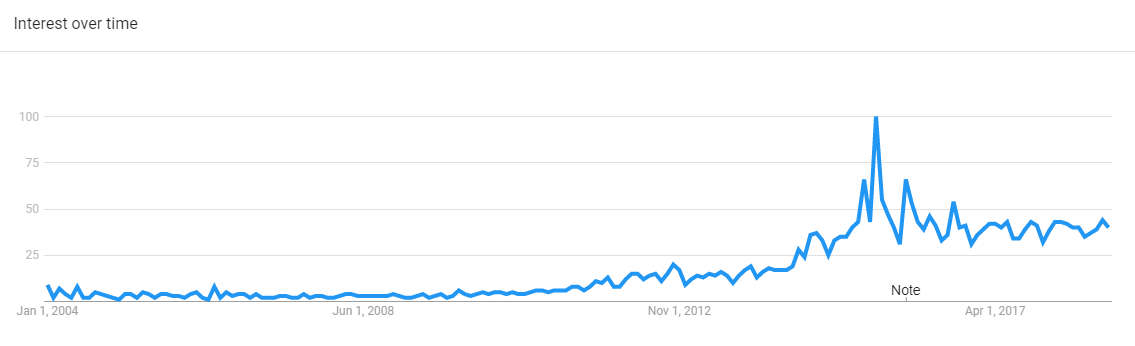
\includegraphics[width=1\textwidth]{figuras/chap-introduction/trends.png}
\caption{Evolution in the number of searches about the term Smart City in Google from 2004 to 2018}
\label{fig:trends}
\end{figure}

Besides tests and experiments of Smart Cities solutions, the simulator can also help city governments verifying the impacts of a myriad of actions in the city such as the building of a new bridge, of a new subway line, and changes in the bus lines itinerary. To evaluate the impact of these actions in the entire city, it is essential to provide a very-scalable simulator able to simulate the whole transportation infrastructure of the city, including the road network, subway network, and bus system. Most of the current open source and proprietary simulators can represent just a small area and with a limited number of agents. 
\section{Objectives and Challenges}
\label{sec:consideracoes_preliminares}

The primary objective of this work is design, implement, and evaluate the development of a large-scale Smart City simulator. The simulator must enable the simulation of a city with millions of actors in an extensive area such as the city of S\~ao Paulo with more than 11 million inhabitants, 4 million cars, 15 thousand buses, and 48 thousand streets in an area of more than 1,000 km\textsuperscript{2}. It is also objective of this work provide tools to facilitate the development of simulation scenarios using real data such as the map of the city, origin-destination surveys, and buses time-tables. The simulator also must generate output data that are easy to analyze and visualize.

A secondary objective is to show that the simulator is useful for different activities in Smart Cities projects. For example, the test and experiments of Smart City applications and platforms, to evaluate the infrastructure of a city, and as a testbed for new city simulation models.

To execute a simulation with the desired scalability, we had to solve many computational challenges. The first challenge was to select the right language and tools that enable the implementation of highly scalable software. Also, we had to test many data structures and algorithms to support the simulation scale. This research was necessary because most of the current simulators enable the simulation of just hundreds or thousands of simultaneous objects because of problems in their architecture. To simulate a city with the size of S\~ao Paulo in a reasonable time it is required a highly scalable and efficient implementation.

To achieve the necessary scalability, we developed a simulator able to execute parallel and distributed simulations. It adds yet more complexity to the implementation of the simulator because some of the models used in the simulator were never used in parallel implementations. To facilitate this task, we used Erlang, a language that promotes the development of scalable parallel and distributed applications. 

Finally, developing simulation models consistent with reality is also a challenge. To solve this problem, we made extensive research of different models and algorithms used to simulate cities such as traffic and public transportation models. We also used a lot of real-data such as maps and origin-destination surveys to further the realism of the simulations.

\section{Research Questions}

Our work involves answering the following three research questions:

\begin{description}
\item[RQ1:] ``What are the requirements to develop a general purpose, scalable Smart City simulator?''
\item[RQ2:] ``What is the most suitable programming model for the development of a large-scale Smart City simulator?''
\item[RQ3:] ``What are the possible uses of a large-scale Smart City simulator?''
\end{description}

To answer RQ1, we conducted a literature review of Smart Cities and related simulators. With this review, we identified the functional and non-functional requirements that a Smart City simulator should handle. For example, the simulator must represent the city map in an efficient data structure and allow a straightforward definition of the travels that must be simulated. 

To answer RQ2, we developed a Smart City simulator using Erlang, a language that implements the actor model and performed experiments to evaluate the simulator scalability. The evaluation shows that the simulator handles more than 20  millions actors efficiently in a single simulation executing faster than real-time.

Finally, to answer RQ3, we present the contexts that InterSCSimulator were already used and also describe other possible uses of the software. For example, the simulator was used to analyze the scalability of a Smart City platform and to compare mobility scenarios in the city of s\~ao Paulo.

\section{Thesis Organization}
\label{sec:organizacao_trabalho}

This thesis is organized as follows. Chapter \ref{cap:conceitos} presents the fundamental concepts used in this thesis which are Smart Cities, Traffic Simulation, and the Actor Model. Chapter \ref{cap:relacionados} cites related work including simulators of different domains of Smart Cities. Chapter \ref{cap:interscsimulator} introduces the development of InterSCSimulator, showing the functional and non-functional requirements, architecture, components, and implementation evolution. Chapter \ref{cap:sao_paulo} presents the simulation of the city of S\~ao Paulo, with more than 20 million travels, which served as the base for the scalability evaluation of the simulator. Chapter \ref{cap:avaliacao} presents the scalability evaluation of the simulator, showing experiments regarding its execution time and resources usage. Chapter \ref{cap:uses} presents examples of research already supported by the InterSCSimulator. Finally, Chapter \ref{cap:conclusoes} discusses the results of this thesis and future work.
\par

\chapter{Fundamental Concepts}
\label{cap:conceitos}

This chapter presents the main base concepts used in the development of this work. Section \ref{sec:cidadesInteligentes} presents definitions and dimensions of Smart Cities and possible simulation scenarios. Section \ref{sec:simulacaoTransito} describes the fundamentals of traffic simulation, highlighting the types of traffic simulations and examples of Smart Cities scenarios already simulated. Section \ref{sec:modeloAtores} presents the actor model and the Erlang language which we used in the implementation of the InterSCSimulator. Finally, Section \ref{sec:rev_conclusoes} concludes this chapter, relating the presented concepts and the research presented in this thesis.

\section{Smart Cities}
\label{sec:cidadesInteligentes}

Most of the Smart Cities definitions highlights the expected impacts of innovative services and applications in the city population and the environment such as citizens empowerment, better quality of life, and sustainability. Other, focus on the idea of using ICT tools to create and improve the cities infrastructure and services. Table \ref{tab:definicoes} presents Smart Cities definitions that we found in the literature. Most of these definitions cite that the primary objective of a Smart City is improving the citizen quality of life. Some definitions \citep{giffinger2007smart,guan2012smart} do not establish the mean to achieve this objective, while others define that this objective will be achieved using a technological infrastructure to improve the infrastructure and services of the city \citep{caragliu2011smart,dameri2013searching,harrison2010foundations}.

\begin{table}
\centering
\caption{Smart Cities definitions found in the literature}
\label{tab:definicoes}
\smallskip
\begin{tabular}{c|c}
\hline

Definition 
& Author \\\hline

“A Smart City is a city well performing built on the\\
‘smart’ combination of endowments and activities of\\ 
self-decisive, independent and aware citizens” &  \citep{giffinger2007smart} \\\hline

“A city to be smart when investments in human and social\\
capital and traditional (transport) and modern (ICT)\\
communication infrastructure fuel sustainable economic\\ 
growth and a high quality of life, with a wise management\\
of natural resources, through participatory governance”
& \citep{caragliu2011smart}  \\\hline

“A smart city is a well-defined geographical area, in which\\
high technologies such as ICT, logistic, energy production,\\ 
and so on, cooperate to create benefits for citizens in terms\\
of well-being, inclusion and participation, environmental\\
quality, intelligent development; it is governed by a\\ 
well-defined pool of subjects, able to state the rules and\\ 
policy for the city government and development” 
& \citep{dameri2013searching}  \\\hline

“A city that monitors and integrates conditions of \\
all of its critical infrastructures, including roads, \\ 
bridges, tunnels, rails, subways, airports, seaports, \\ 
communications, water, power, even major buildings, \\
can better optimize its resources, plan its preventive \\
maintenance activities, and monitor security aspects \\
while maximizing services to its citizens”
& \citep{hall2000creative} \\\hline

“A city connecting the physical infrastructure, the\\
IT infrastructure, the social infrastructure, and the\\
business infrastructure to leverage the collective\\
intelligence of the city”
& \citep{harrison2010foundations} \\\hline

“A smart city, according to ICLEI, is a city that is\\ 
prepared to provide conditions for a healthy and happy\\
community under the challenging conditions that global,\\
environmental, economic and social trends may bring.”  & \citep{guan2012smart} \\\hline

“The use of Smart Computing technologies to make the\\ 
critical infrastructure components and services of city\\
which include city administration, education, health-care,\\ 
public safety, real estate, transportation, and utilities\\
more intelligent, interconnected, and efficient”
& \citep{washburn2009helping} \\\hline

\end{tabular}
\end{table}

Most of the Smart Cities definitions cite the necessity of using Information and Communication Technologies (ICT) to improve the use of the city infrastructure, the resources management, and the city services \citep{harrison2010foundations,washburn2009helping}. Some definitions also cite the importance of sustainability in the city, making more efficient use of resources such as water and electricity \citep{caragliu2011smart,dameri2013searching}.

Another important discussion is the necessity of leveraging the economic development of the cities \citep{dameri2013searching}, facilitating the integration and participation of the whole city population. Two definitions \citep{dameri2013searching,giffinger2007smart} cite the importance of participatory governments allowing the citizens define the cities priorities.

Also regarding ICT, some definitions cite that Smart Cities applications and services should monitor the cities infrastructure such as streets, bridges, train lines and stations, and public buildings \citep{hall2000creative}. Also, they must monitor and control their resources such as water and electricity \citep{hall2000creative}. Finally, the data collected in the city monitoring must be available and integrated to facilitate the creation of Smart Cities applications and services \citep{harrison2010foundations,washburn2009helping}.

Besides the Smart Cities definitions, Giffinger et al. \citep{giffinger2007smart} describe six dimensions to measure the smartness of a city. The dimensions are: \textit{Smart Economy}, \textit{Smart People}, \textit{Smart Governance}, \textit{Smart Mobility}, \textit{Smart Environment} and \textit{Smart Living}. Many authors already use this classification \citep{munoz2011forefront,papa2013towards} and there is a benchmark used to rank the smartest cities in Europe using these dimensions.\footnote{Smarts Cities in Europe - \url{www.smart-cities.eu}} The definition of each dimension is in the following:

\begin{itemize}

    \item \textbf{Smart Economy} measure the economic development of the city through parameters such as the quality of the enterprises in the city and the city entrepreneurship ecosystem. Examples of initiatives related to this dimension are incentives to companies for the development of technological solutions for the city and the improvement of the business environment with adequate legislation and business infrastructure. 
    
    \item \textbf{Smart People} is related to the development of the city's population using parameters such as education, employment rate, and income. Some actions related to this dimension are projects for digital inclusion of citizens and programs for scientific and technological education. 
     
    \item \textbf{Smart Governance} access the quality and transparency of municipal public agencies with parameters such as ease of use of public services, investments in technology, and transparency in the public data and the use of city resources. Some actions related to this dimension are the creation of participatory governments and the dissemination of information about the city in transparency and open data portals.
 
    \item \textbf{Smart Mobility} measures the ease of mobility in the city in the various modes of transportation such as bus, subway, car, and bicycle. It uses parameters such as kilometers of congestion, subway network size and the number of people using public or non-polluting transportation. Some actions related to this dimension are real-time monitoring of streets flow, the use of sensors to indicate free parking spots and applications to facilitate and encourage the use of public and sustainable transport, such as bicycles and electric vehicles.
 
    \item \textbf{Smart Environment} check the sustainability of the city using parameters such as environmental pollution, efficiency in the use of city resources such as water and electricity, and the amount of recycled waste. Some actions related to this dimension are the measurement of the city's air and water quality, the use of renewable energy sources and the real-time measurement of the resources used in buildings.
    
    \item \textbf{Smart Living} evaluates the quality of life of the population using parameters such as entertainment, security, and culture. For example, counting the number of green areas, the number of libraries and homicide rate of the city. Some actions related to this dimension are the use of elderly health monitoring applications, automatic image processing of security cameras and applications that show the cultural events programmed in the city.

    
\end{itemize}

There are a plenty of Smart Cities initiatives around the world, most in Europe \citep{caragliu2011smart,manville2014mapping}, several in the United States \footnote{10 Smartest Cities in USA - \url{www.fastcoexist.com/3021592/the-10-smartest-cities-in-north-america}}, Japan and China \citep{liu2013smart} and some other project in other countries such as Brazil \citep{fortes2014deployment}, United Arab Emirates \citep{janajreh2013wind} and South Korea \citep{kshetri2014development}. These data show that the vast majority of projects are concentrated in developed countries, there are a few projects in developing countries. In Brazil, there are already several initiatives such as in S\~ao Paulo, B\'uzios, Recife, and Joinville. We did not find any project in the poorest countries of the globe. Figure \ref{figure:mapa} shows a map of the initiatives found in the literature or pages of the projects.

\begin{figure}[!htb]
\centering
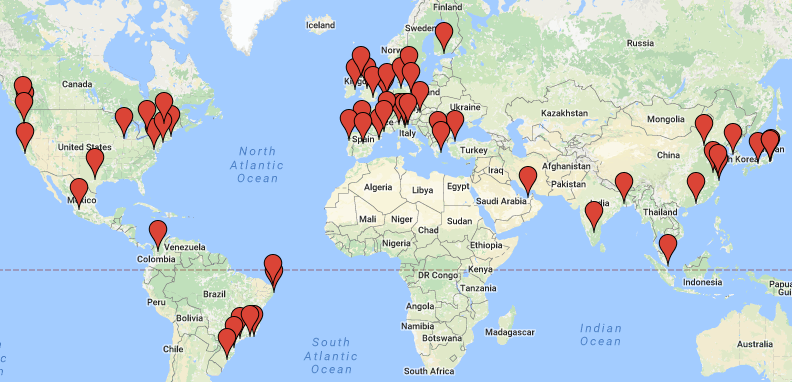
\includegraphics[height=7cm]{figuras/mapaCidades}
\caption{Smart Cities initiatives around the world}
\label{figure:mapa}
\end{figure}

Some examples of very advanced initiatives in Smart Cities are Santander, Spain, which through the SmartSantander project has already deployed an extensive sensor network in the city to collect data such as temperature, vacant parking spot and noise levels in the city streets. Amsterdam, which has a variety of Smart Cities projects such as encouraging the use of electric cars, bicycles and public transport, automatic monitoring of the city conditions and the use of a smart electricity distribution network. Barcelona, Spain, which has several projects to increase citizens' participation in city decision-making and to make data available on public administration openly.

The next sections present Smart Cities initiatives, applications, and services already implemented in cities around the world. Based on these initiatives, we derived possible scenarios that are possible to simulate in a Smart City simulator.

\subsection{Smart Economy}

This subsection presents projects related to the economic growth of the city, attracting investments and creating more and better jobs. Examples of services and applications of this field are associated with tourism, efficient usage of city resources and the attraction of enterprises and startups to the city. 

In Santander, researchers developed an augmented reality application to smartphones which contain plenty of information of more than 2700 points of interest in the city such as museums, bookstores, buses stop, tourism office, and bicycle rental stations. The application also shows the position of buses and taxis in real-time \citep{sanchez2014smartsantander}. Figure \ref{figure:santanderRa} presents the main screen of the applications, which shows the information of a bus line and a point of interest of the city.

\begin{figure}[!htb]
\centering
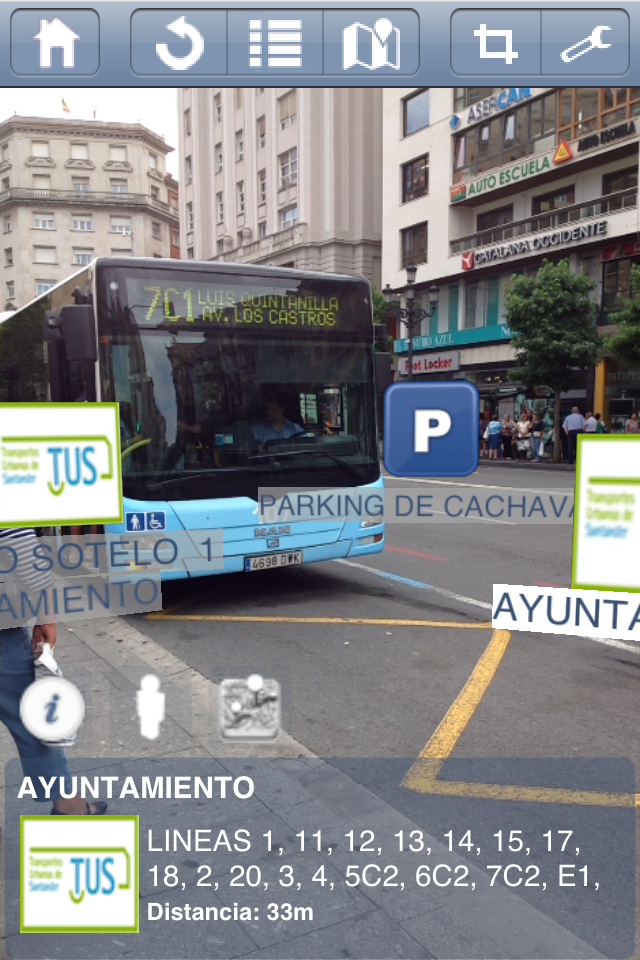
\includegraphics[height=10cm]{figuras/santanderRA}
\caption{SmartSantander augmented reality application}
\label{figure:santanderRa}
\end{figure}

In Cagliari, Italy, the municipal government has developed a platform based on the Internet of Things and Cloud Computing to collect data and create services for tourists in the city \citep{nitti2017iot}. To test the platform, they developed a case study in which a tourist selects a list of Points of Interest (POIs) that they want to visit in the city. Each PdI has a variety of static data, such as address and hours of operation, and data captured in real time, such as the size of the entrance queue and the current number of visitors. With this data, the application calculates the best sequence of PdIs that the tourist should visit. The purpose of the application is to optimize the time of the tourist, allowing him to be able to visit as many attractions as possible in the time that he is in the city.

Also related to tourism in Amsterdam, the government has adopted the CitySDK Tourism API \citep{pereira2015citysdk}, a tool that allows the development of applications to help tourists visiting the city. This tool collects data from the city's open data portal, which is in CSV, XLS, and text files and makes them available in an easy-to-access and processing API for third-party applications. Some of the shared data are city landmarks such as museums, parks and historic buildings, events that are happening in the city and tourist itineraries.


Búzios is one of the first cities in Brazil to start a project for the implementation of a Smart City infrastructure \citep{fortes2014deployment}. The main purpose of the project is to make the city more sustainable, using resources rationally and efficiently. Among the main actions carried out in the city is the implantation of an intelligent electric energy network, the creation of intelligent buildings and the improvement of the communication systems of the city using technologies such as Wi-Fi, Mesh networks, and Power Lines Communication (PLC).

Also in Amsterdam, the government deployed the first Smart Electricity Grid in a region of the city with approximately 10,000 houses. In this network, it is possible for c to consume and produce energy and to monitor energy usage in their homes in real time. Also, this project also facilitates the monitoring and maintenance of the network by city authorities.

In this application domain, researchers can develop simulations of a Smart Grid, comparing the cost and the emission of pollutants in the use of diverse sources of electrical energy and simulating the network of distribution, production, and consumption of energy. They can also simulate buildings that attract large numbers of people, such as sights and places of big events, making it possible to understand their impacts on the city's traffic.

\subsection{Smart Population}

This subsection presents projects aimed at improving social parameters related to the population of the city such as education, employment, and income. Moreover, some researchers discuss the empowerment of citizens with data that allow them to make better political choices. Examples of services and applications in this area are related to education such as initiatives and applications for improving education and facilitating the digital inclusion of city citizens and improving the city's business environment by increasing the quantity and quality of jobs.

An initiative in England teaches students to work with data sets related to the city \citep {wolff2015education}. The idea is to enable citizens to know the tools to analyze the data independently of the will of companies or city rulers. The purpose of this work is to extend class activities with activities such as Hackathons aimed at the development of applications and services for the city. The researchers already did tests using datasets on the use of electricity in the city.

In Barcelona, the municipality created a laboratory (Barcelona Urban Innovation Lab Dev), which investigates various urban problems and fosters the participation of the private sector in the development of products and services related to the improvement of urban space \citep {bakici2013smart}. The laboratory provides human resources and tools to support the development of these solutions. The objective of this laboratory is to attract companies to develop tools for the city, creating jobs that need high qualification and also creating solutions to improve quality of life in the city.

Scenarios linked to education can be simulated in this area such as schools and universities, and from which part of the city these institutions attract the population. So governors and private schools can choose the best area for the creation of new schools or university campuses and also measure the impact on the city traffic.

\subsection{Smart Governance}
\label{subsec:governanca}

This subsection presents projects related to the governance of the city. The main objectives of this type of projects are facilitating the city administration and enable the citizen participation in the city decision-making. Examples of services and applications in this field are platforms to city monitoring, open data portals, and the encouragement of the citizens to participate in the city decisions.

Seattle is considered by some rankings the smartest city in the United States \footnote{\url{https://goo.gl/5xAhh9}}.
There, researchers performed a survey \citep{alawadhi2013aspirations} with citizens and public agents asking what the main services, applications, and initiatives that the city are developing to improve the citizens' quality of life are. Among the cited projects are the open data portal \footnote{Seattle Open Data - \url{data.seattle.gov}}, the infrastructure to support the use of electric vehicles, and the use of Customer Relationship Management (CRM) to control the communication between the city government and the citizens. According to the survey, the benefits of these actions are the improvements in the city services, the reduction of the city expenses, and electrical energy saving. 

In Chicago, the municipality developed the platform WindyGrid \citep{thornton13windygrid}, which collects, stores, and process the data of the city. The objective of this platform is providing a unified platform to city operators visualize the city operation in real-time. Examples of the collected data are calls to the emergency service (911), events in the city traffic, publications about the city in social networks, and data regarding the public buildings. The WindyGrid provides three main functional requirements to the city managers: incidents monitoring though emergency calls and social networks mining, historical data visualization, and real-time analyses of events in the city.


In Amsterdam, there are many projects to leverage the city management transparency, especially the city expense and the decisions of the city government. For example, the Budget Monitoring allows citizen and NGOs access and suggest changes to the city budget and the Smart City SDK, which provides access to the real-time city data to application developers, including data about the city traffic, airports arrivals and departures, and the climate. Finally, to facilitate the participatory government, the city developed the AmstermOpent, a platform that allows the citizens to suggest actions and works in the city.

Many cities around the world already provide access to the city documents through open data portals allowing citizens to supervise the government expense and actions. For example, Barcelona\footnote{OpenData BCN - \url{opendata.bcn.cat/opendata/ca}} make available a big number of data about the city administration such as the city budget and expenses, municipal services stats, and data about the city population. Dublin, in Ireland, also has a completely open data platform called Dublinked \citep{stephenson2012open} which provide access to more than 200 datasets offering historical and real-time data. Moreover, using Web Semantic tools, it is possible to link the data from the platform automatically.

S\~ao Paulo has many open data projects such as the open data portal of the city \footnote{Dados Abertos São Paulo - \url{saopauloaberta.prefeitura.sp.gov.br}}, and GeoSampa\footnote{GeoSampa - \url{geosampa.prefeitura.sp.gov.br}} which provides different georeferenced datasets such as the location of public equipment, buses stops, and flood points in the city. Another example is the Olho Vivo API \footnote{API Olho Vivo - \url{www.sptrans.com.br/desenvolvedores/APIOlhoVivo.aspx}}, which allows the monitoring in real-time of all the buses in the city. This API allowed the development of many applications to facilitate the mobility in the city by buses such as Moovit\footnote{Moovit - https://goo.gl/FMYk8u} and Coletivo\footnote{Coletivo - https://goo.gl/QBvoNc}.

Another tool extensively used by the cities to share their data with the citizens is the dashboards. Usually, these tools present real-time data in a city map with various information about the city such as climatic conditions, air quality, traffic conditions, and state of the public equipment. One dashboard example is the Dublin dashboards\footnote{Dublin Dashboards - \url{www.dublindashboard.ie}}, which provides different data about the city such as temperature, air quality, noise levels, and level of the rivers in the city. Figure \ref{figure:mapaDublin} presents an example of the city dashboard displaying data of the city traffic.

\begin{figure}[!htb]
\centering
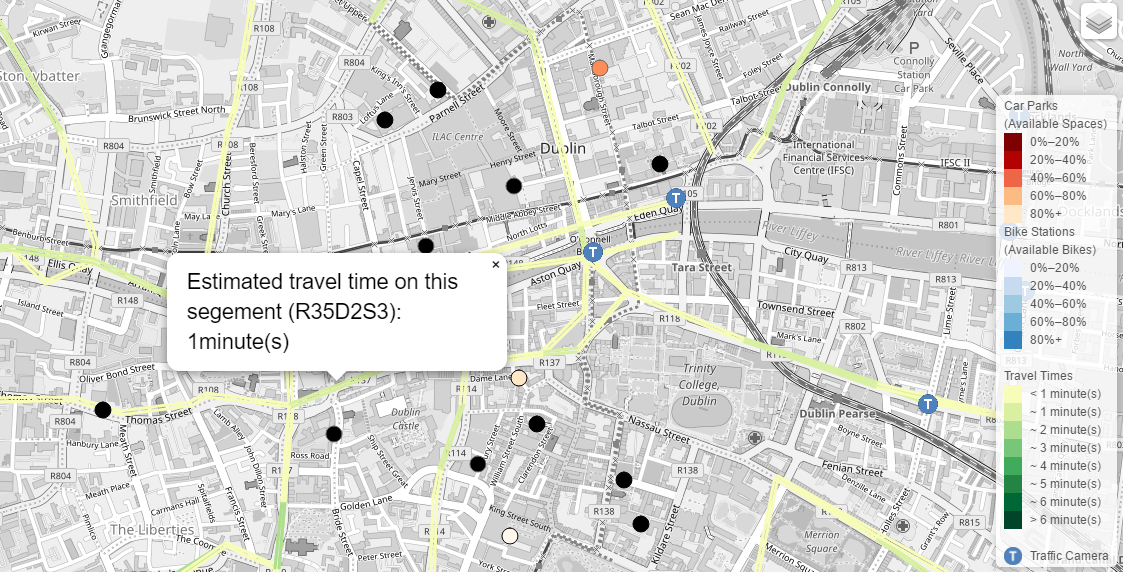
\includegraphics[scale=0.5]{figuras/mapaDublin}
\caption{Dublin Dashboard showing available park spots, available bikes in bikes stations, and the traffic situation in avenues in the city}
\label{figure:mapaDublin}
\end{figure}

This Smart City domain is linked to tools for monitoring the city, and we did not think in any scenario that can be simulated. However, a Smart City simulator can assist in tests and experiments of applications cited in this subsection, enabling the generation of workloads such as sensor and traffic simulation for the creation of monitoring applications.

\subsection{Smart Mobility}

This subsection presents projects related to mobility, which has the main objective of improving the people flow in the city and monitor the mobility infrastructure of the city such as roads and subway stations. There are plenty of examples of Smart Mobility services and applications such as traffic monitoring through security cameras, best route services, smart parking applications, and applications to show the best route using public transportation.

With the SmartSantander platform, a research project developed an infrastructure to show the free parking spots in the city. Moreover, it creates a service to predict the use of the spots during events in the city \citep{vlahogianni2014exploiting}. This service has the objective of avoiding that drivers lose time searching for a parking spot in the city, what increases the traffic in the city and the emission of polluting gases. Figure \ref{figure:smartsantandermap} presents the monitored parking spots in the city map.

\begin{figure}[!htb]
\centering
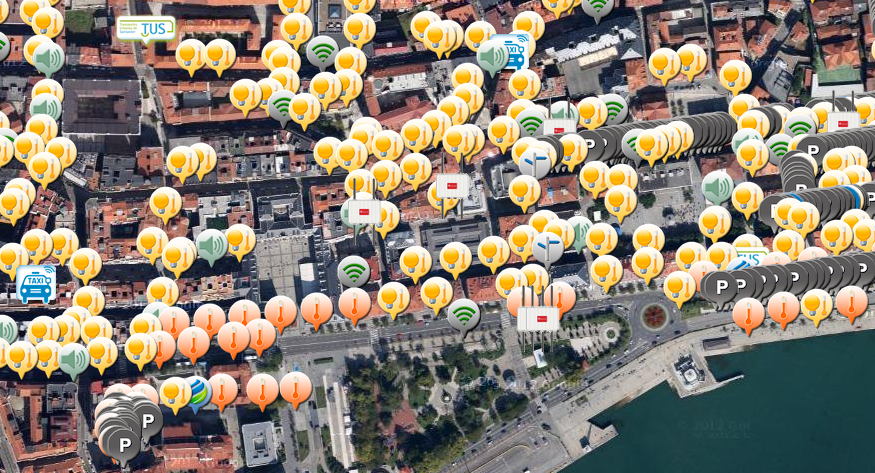
\includegraphics[height=8cm]{figuras/smartsantandermap}
\caption{Map with the monitored parking spots in the city of Santander}
\label{figure:smartsantandermap}
\end{figure}

The city of Barcelona also has a project to encourage the use of sustainable transportation modes. For example, the city developed a large infrastructure to facilitate the use of electric cars with more than 300 recharge points deployed in the city. Moreover, the city is promoting the use of shared bicycles and provided more than 400 loan stations to the citizens.

Amsterdam is also implementing several solutions in the area of traffic control and monitoring. For example, projects under development in the city are: encouraging the use of electric cars, providing battery recharging stations in various parts of the city, monitoring the main city roads for the rapid attendance of traffic problems, reservation of parking spaces in the city, avoiding the search for a vacancy, reducing the emission of $CO_2$, and the incentive to use bicycles.

In Madrid, researchers developed other two projects. The first was an application to smartphones to facilitate the commuters to find the best route using public transportation in the city. The applications also used contextual information to find best routes such as the user location and the city weather. The second application uses the user's smartphones to estimate the number of people inside a bus. People expecting for a bus can use this information to decide if it worth to take the bus or wait until the next one.

In S\~ao Paulo, the startup Scipopulis \footnote{Scipopulis - www.scipopulis.com} developed a Bus Panel used by the São Paulo Transport Secretariat (SPTrans) and the Company of Traffic Engineering (CET). This application monitors the more than 14,000 city buses and shows the speed of buses in real time on all the streets and integrates data from various sources (GPS positions of buses, segregation of the road, accidents, etc.). This information is contextualized regarding the time of day, type of road (corridor, track or shared road), accidents in the region and amount of bus passing through that route. The operator can monitor entire bus lines or sections of a line, and view the history of speeds for each street segment. The city transport network planning, operation and management teams use the panel to identify chronic bottlenecks, contingency problems, identify ways to implement buses single lanes and corridors, and the times at which the buses should operate. Figure \ref{figure:scipopulis} shows a screen of the Bus Panel application.

\begin{figure}[!htb]
\centering
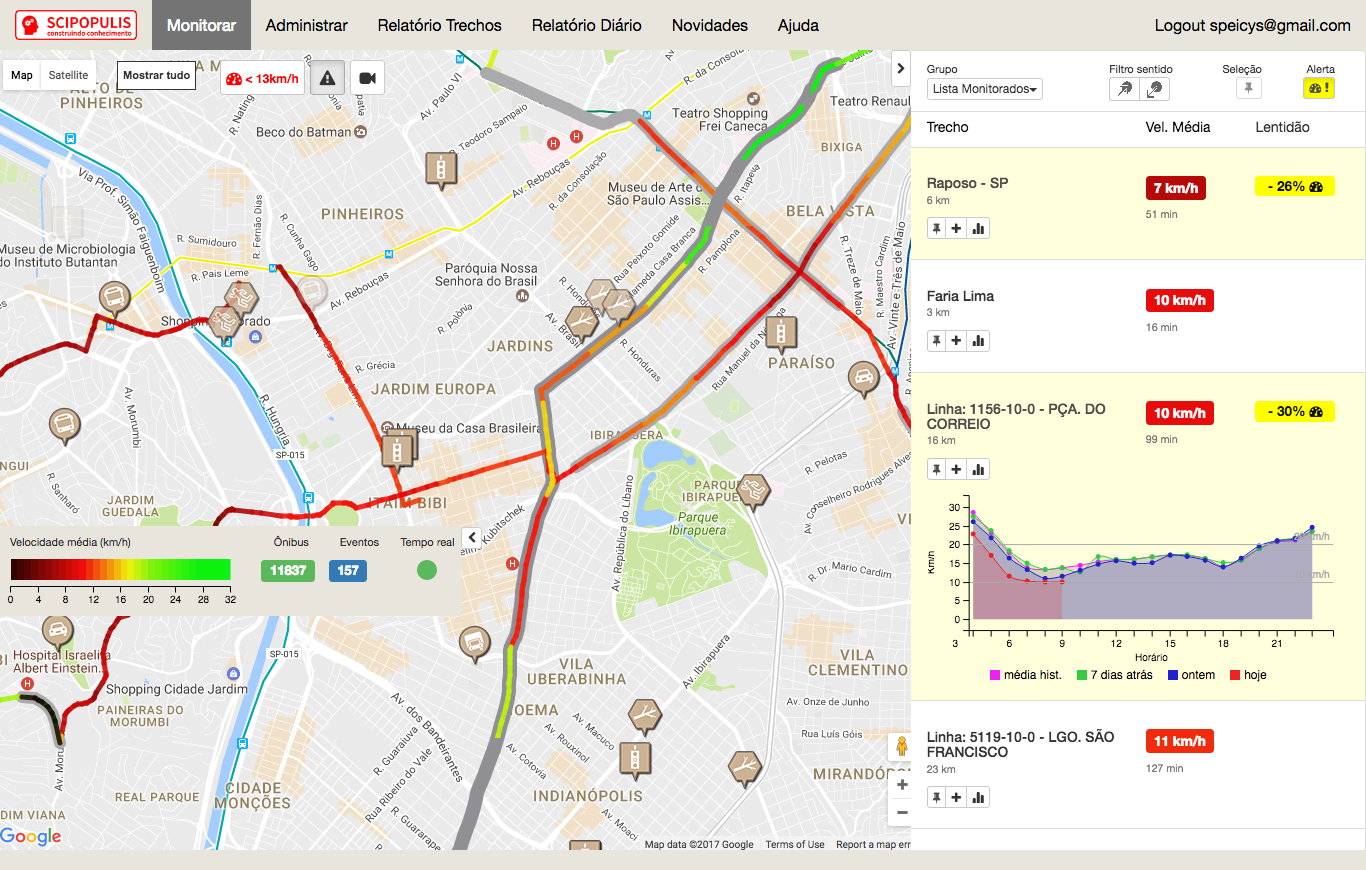
\includegraphics[scale=0.30]{figuras/scipopulis}
\caption{S\~ao Paulo bus dashboard showing the speed of the buses in the main avenues and bus corridors in the city}
\label{figure:scipopulis}
\end{figure}

In the dimension of Smart Mobility, it is possible to simulate a large number of scenarios such as the movement of vehicles in the city, compare various parameters in the road network such as increasing or decreasing street speed, accidents, and problems in roads such as floods or protests. It is also possible to simulate the public transportation of the city such as buses and subways, comparing the city traffic by increasing or decreasing the number of users on public transport, searching for the best route to a new bus line and analyzing the impact of new subway lines.

\subsection{Smart Environment}

This subsection presents projects related to the environment. Most of them have the objective of making the city more sustainable improving services such as garbage collection and recycling, efficient distribution of resources such as water and electricity, and reducing air and water pollution in the city.

Masdar is a neighborhood in the city of Abu Dhabi in the United Arab Emirates built with the objective of testing several initiatives of Smart Cities. The areas tackled in the project are the use of renewable energy sources, the conscious use of water and the reduction of the amount of garbage generated. Also, the city was planned with an intelligent transportation network to reduce the need for the use of individual vehicles, reducing the emission of pollutants. In this neighborhood, all buildings are designed in a way that saves resources and produces their energy with the use of solar panels.

In Manchester, the city is developing a project to build smart houses. In this houses, the citizen can monitor in real-time the use of resources such as electric energy and water. The objective of this project is to decrease the pollution emission and save the natural resources of the city \citep{manville2014mapping}.

The city of Santander has implemented a project to manage garbage collection in the city\citep{munoz2017santanderlixo}. This project uses data from more than 1000 sensors that monitor how full the city dumps are. Also, it is possible to monitor garbage trucks and garbage dumps. This system allows garbage trucks to visit only dumps that are full, reducing the distance that the trucks must travel. Three significant benefits of this service are the decrease in the truck expenses, the reduction of emissions of pollutants by the vehicles and the better management of the garbage collected in the city. Barcelona also has a similar project in which it is possible to monitor the current state of the garbage dumps in the city. Figure \ref{figure:sentilo} shows the city map with the sensors in the dumps.

\begin{figure}[!htb]
\centering
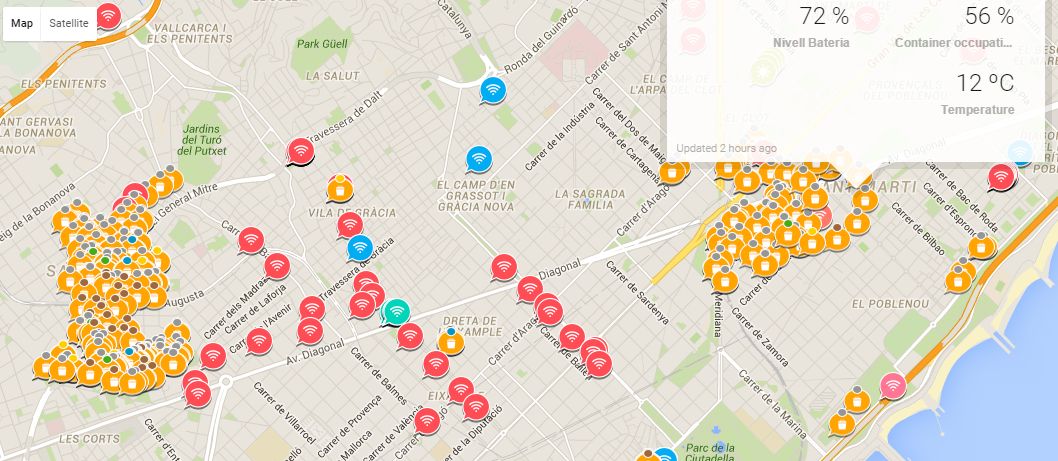
\includegraphics[scale=0.5]{figuras/sentilo}
\caption{Sensors indicating the amount of garbage in the city dumps in the Sentilo platform}
\label{figure:sentilo}
\end{figure}

Also in Santander, the city is deploying a Smart Light project, which installed more than 20.000 LED lamps with a movement detection system. This system turns on the lamp only when it detects a person is moving close from the lamppost. Also, along with the system, the smart lamps also allow the monitoring of the state of the lamp, facilitating the detection of problems in the system. With this project, the city plans to reduce 80\% the electric power consumption with the public lighting. Also, the city expects to reduce the expenses with the maintenance of the system, because currently the maintenance is made through rounds across the city.

A district of Barcelona is already operating a system for heating and cooling buildings \citep{hug2016barcelona}. The system works with a water network that passes through several district buildings, mainly public building and using the energy generated by the city's waste incinerators heat or cool the water in the pipeline. The city estimated that this system uses 35\% less power and reduces pollutant emissions by 50\% than conventional systems heating systems.

In the dimension of Smart Environment, it is possible to simulate the impact of different initiatives in the environment. For example, the emission of pollutants by the car fleet of the city, the variation in the emission if more people use public transportation, and the impact of using electric vehicles. Also, it is possible to simulate the environmental impact of the use of different electric power sources such as hydroelectric, wind, and solar. 

\subsection{Smart Living}

This subsection presents projects related to the improvement of citizens' quality of life. These project aims to improve services that are directly related to citizens' routine, such as security, cultural activities and sports activities. Examples of services in this dimension are applications that warn of events taking place in the city, for monitoring crowded areas, and for reporting problems in public places such as parks and government buildings.

In Santander, researchers installed a network of more than 20 thousand sensors and actuators in the city. This sensor network collects a vast amount of data in various regions of the city such as temperature, free parking spaces, points of interest and luminosity. The data collected is used for the development of applications and services that improve the quality of life of the citizens. Figure \ref{figure:smartsantandermap} shows a map in which each point is a device deployed in the city that sends data to the platform. An example of an application developed with the data of the sensor network is one that reminds the city population of events that will occur in the city. Besides the event, the application also sends information about the region of the event to the users such as parking spots, noise levels, and temperature.

In Dublin, in the same dashboard presented in Section \ref{subsec:governanca} the city provides in real-time the stream of surveillance cameras in different areas in the city. These videos allow the monitoring of various problems that can occur in the city such as traffic accidents, crimes, and health issues. Also, developers can use these video stream to the development of applications in the city to automatically monitor the city conditions such as level of the rivers and traffic problems.

The data used in the applications and services presented in this section are about activities that will occur and streams of surveillance cameras captured in real-time in the city. In this domain, it is possible to simulate the deployment of a sensor network in the city, allowing the comparison of the costs and coverage area of the network depending on the number and type of the sensors. This simulation can also be very useful to the tests and experiments for Smart City applications and services. 

\section{Traffic Simulation}
\label{sec:simulacaoTransito}

One of the main components of a Smart City simulator is the traffic model because it controls the way the city road infrastructure is implemented. For example, it is possible to model the city as a matrix or using a digraph. This section presents concepts of traffic simulations including the city, vehicle, and people representation. Moreover, we describe the most common traffic models used in the literature: microscopic, mesoscopic, and macroscopic. These three types of traffic simulation differ mainly in the detail level of the simulation \citep{barcelo2010fundamentals}. The main characteristics of each type of traffic model are:

\begin{description}

\item[Microscopic:] Microscopic simulators model each vehicle individually and to calculate the speed of the vehicle they used mathematical models that consider the behavior of each vehicle about the other vehicles. In the literature, we found two most common models, the \textbf{Car Following Model}, which calculate the speed of the vehicle according to the speed of the vehicles in front of it and the \textbf{Lane Change Model}, which models when a vehicles change the lane in the street. This type of simulation is usually used to understand the behavior of small areas in a city such as intersections and rotations.

\item[Mesoscopic:] Typically, the mesoscopic models also model each vehicle individually. However, the speed of the vehicle in a particular path is calculated by a density function that usually considers the length and number of lanes of the road to calculate its capacity.  Researchers normally use macroscopic models for simulating large areas such as a neighborhood and even whole cities.

\item[Macroscopic:] Macroscopic models model the transit of a region as flows in a road network. This type of simulation does not consider individual vehicles and speeds are also calculated by functions that analyze the size of the vehicles flow on the road over a given period. There are macroscopic simulators capable of simulating a road network of an entire country.

\end{description}

Among the types of traffic simulation presented, the mesoscopic models are the more suitable for this work. For a Smart Cities simulation, it is necessary to model individual vehicles for analysis and model scenarios for application and platform testing. However, there is no need to model in detail the interaction between the vehicles, as the microscopic models do. Another significant advantage of mesoscopic models over microscopic models is that in mesoscopic models it is possible to implement simulators capable of modeling large urban areas such as the metropolitan region of a large city such as São Paulo and New York.

Examples of Smart Cities scenarios already implemented in mesoscopic traffic simulators are:

\begin{description}

\item[Electric Vehicles:] Many traffics simulators were used to simulate electric vehicles and the required changes in the city infrastructure to support the growth in the energy demand. In these simulations, the researchers modified traffic models to simulate the energy consumption of the vehicles and implemented models to simulate the city infrastructure such as recharge points and renewable energy sources \citep{allan2015benchmark,geske2010modeling}. 

\item[Emission of Pollutants:] Some traffic simulators include a pollutant emission model, calculated using the type of the vehicles, the traffic, and the traveled distance in each simulated travel \citep{xia2005modelling,hulsmann2014modelling,krajzewicz2012recent,zhou2015integrating}. Usually, a mathematical formula is used to calculate the amount of $CO_2$ and other pollutants emitted by each travel. Different researchers can be performed using this model. For example, researchers can measure the impacts in the environment of the increase in the use of the public transportation and bicycles.
 
\item[Vehicular Networks:]  There are many simulators used to the simulation of vehicular networks, simulating Vehicle-to-Vehicle (V2V) and Vehicle-to-Infrastructure - (V2I) communications. For example, the RedSwarm project \citep{stolfi2014red} has the objective of developing new routing algorithms using real-time data to reduce the vehicles travel time. In this project, many devices deployed in different regions of the city measure the traffic conditions and communicate with the vehicles indicating their best route. Besides, V2V communications are used for the propagation of messages about problems in the roads. To test the algorithms developed in the project, the researchers used the traffic simulator SUMO \citep{behrisch2011sumo}.


\end{description}

\section{Actor Model and Erlang}
\label{sec:modeloAtores}

The Actor Model \citep {de2014dealing} is a robust model for the development of highly concurrent and distributed applications. In this model, each actor is an independent processing unit that has its memory area. Actors can communicate only through asynchronous messages. Each actor has a message box in which all the messages that the actor receives are stored until the actor processes it. After receiving a message, an actor can change his internal state, reply it, or create new actors.

This model minimizes two significant problems of concurrent systems: \textbf{Race Condition}, because the actors do not share state or resources, so there is no need for synchronizing mechanisms such as traffic lights or monitors. \textbf{Busy Waits}, because all communication between the actors is through asynchronous messages. Although the actor model is an old idea (defined in 1985) \citep {agha1985actors}, this model has been gaining popularity in recent years due to multi-core architectures and ease of development of distributed applications.

As well as the implementation of competing applications, the Erlang language facilitates the development of distributed applications. It is possible because in the Actor Model there are no differences if the actors are running on the same or different machines. The only requirement for distributing the application is that languages based on the actor model should allow the exchange of messages from actors who are running on different machines transparently. Currently, several languages are based on the model of actors like Erlang and Scala \citep{tasharofi2013scala}, and many others have an implementation for the actor model such as Ruby \footnote {Celluloid - \url{celluloid.io}}, and Java \footnote{Reactors.io - \url{reactors.io}}.

\subsection{Erlang}
\label{sub:erlang}

Erlang is a functional programming language based on the actor model. It was developed meanly to facilitate the implementation of parallel, distributed, large-scale software. The language was created by Ericsson\footnote{Ericsson - \url{www.ericsson.com}} in the 80's to the development of telecommunication applications. Currently, Erlang is used in several application domains such as Internet chat \footnote{WhatsApp - \url{goo.gl/If6k3d}}, databases \citep{anderson2010couchdb}, and simulators \citep{song2011performance,toscano2012parallel}.

The main characteristics of Erlang, inherited from the Model of Actors, are quite adequate for the development of large-scale simulators:

\begin{description}

\item[Parallelism:] The Erlang virtual machine allows the creation of a large number of application threads. In the Erlang programming model, each actor created in the application is mapped to an application thread that can perform actions independently of the other actors. Erlang also creates a system thread for each CPU of the computer running the application and balances the actors between those threads to try to maximize CPU utilization.
\item[Distribution:] In the Actor Model, there is no difference whether the actors are running on the same machine or distributed machines making distributed application development transparent to programmers. The Erlang Virtual Machine provides the entire implementation of the exchange of messages among different machines. The only requirement for an Erlang programmer is to create a text file that has the address of all machines on which Erlang actors will run.
\item[Fault Tolerance:] As previously mentioned, each actor Erlang is independent of the other actors in the application. So an error occurred in one actor does not propagate to the rest of the application.
\item[Communication Protocol: ] Erlang actors, as previously mentioned, can only communicate through message exchange, which minimizes the need for mutual exclusion algorithms and tools. The entire communication mechanism, local or distributed, is implemented by the virtual machine, which makes the use of these functionalities transparent to the programmer.
\end{description}

There are some of the disadvantages of using Erlang in the simulator implementation. For example, we must implement the synchronization of the actors, because in Erlang each actor is independent of the other and it is impossible to know the order of execution of threads that execute in parallel. Another problem is the lack of tools for the development of Erlang applications such as Integrated Development Environment (IDE) and test tools.

\subsection{Sim-Diasca}
\label{subsub:simdiasca}

In the InterSCSimulator development, we used Sim-Diasca (Simulation of Discrete Systems of All Scales) \citep{song2011performance}, a general purpose simulator that aims to allow the simulation of large scenarios implemented by EDF\footnote{EDF --- \url{www.edf.fr/content/sim-diasca}}. This simulator is implemented in Erlang, supporting the execution of distributed and parallel simulations.

Sim-Diasca handles all the essential requirements for the execution of discrete-event simulations such as simulation time management, random number generation, events ordering and reproducibility of the results. Besides, it also manages the distribution and parallelism of the simulation actors making loading balancing, creating actors in distributed machines, and handling faults in a distributed environment.

\section{Conclusions}
\label{sec:rev_conclusoes}

This chapter presented the most important concepts used in the development of this work. First, we introduced a literature review about Smart Cities, what was necessary to understand the domains and dimensions of Smart Cities and what is possible and useful to simulate. Then, we presented a review of traffic simulations and the types of simulations that we found in the literature, it was important because the city traffic has an important role in the entire city working. Finally, we presented the actor model and the Erlang language, which were used in the implementation of the simulator, mainly because this language can support the development of large-scale parallel and distributed systems.

Our literature review showed that it is possible to simulate various Smart City scenarios, and these simulations can facilitate the tests and experiments of Smart City solutions. We also discussed why Erlang is a reliable choice for the implementation of the simulator and why mesoscopic simulation is a good alternative to met our objectives. In the next chapter, we will discuss the related work, mainly showing simulators that already provides one or more Smart Cities scenarios.
\par

\chapter{Related Work}
\label{cap:relacionados}

In our literature review and web searches, we found simulators of different city domains such as traffic, smart grids, and soil occupation. Some of them are extensible to simulate complex cities scenarios such as the effect of electric vehicles in smart grids, the use of public transportation in the urban mobility, and the influence of shared cars in the city traffic. This chapter presents simulators that implement at least one smart city domain. We defined the requirements for the development of InterSCSimulator based on the simulators described in this section.

\section{Traffic Simulators}
\label{sec:rel_transito}

As the main implementation of the current version of InterSCSimulator is the traffic , we will first present the traffic simulators found in the literature. These simulators are divided into two types: the microscopic simulators that aim to minutely simulate the behavior of the drivers and the macroscopic simulators that can use mesoscopic or macroscopic models and intent to reproduce the entire mobility system of a large area. Typically, a microscopic simulator considers just a small number of blocks and intend to evaluate the impact of an intervention in the city infrastructure such as a new lane in a street or a new group of semaphores in a neighborhood.

Differently, a macroscopic simulator examines a broader area and aim to study impacts of extensive changes in the city infrastructure such as a new subway line, a new bus corridor, or the effect on the mobility of the city with a new financial district in the city. We will detail three simulators that are more related to our work and then present a list of other projects.

\subsection{MATSim}

MATSim is an open source, agent-based, mesoscopic, traffic simulator \cite{horni2016multi}. In this simulator, each person is modeled as a software agent with individual settings, and the sum of all agents actions have representative demographics of a region \cite{balmer2008agent}. Each agent has a plan which are all the daily activities from the simulated person such as work, university, and leisure. Besides the agents' schedule, to create a simulator scenario in MATSim, it is also necessary a graph that represents the city road network. 

After the creation of the scenario, the simulator executes all the displacements of the agents in the scheduled time using the city road network. The core of the simulator use only pedestrian and car models. However, several works are extending MATSim to the use of buses \cite{fourie2014reconstructing}, autonomous taxis \cite{bischoff2016simulation}, and shared vehicles \cite{balac2018modeling}. 

MATSim uses a queue-based algorithm to simulate the movement and calculate the speed of the vehicles during the simulation. In this model, all the streets are queues in which the cars have to wait a determined time to go to the next street. The flow and storage of the links are limited. If both are free, the vehicles travel in the free-flow speed. Otherwise, their speed is calculated using a density formula. The results are saved in a text file with all the events occurred during a simulation. This file is used to statistical analyses or for the visualization of the simulation.

A significant advantage of MATSim is the offer of several tools to facilitates the creation of simulation scenarios such as a parser of the OpenStreetMap format, a coordinate system converter, a map editor, and a visualization tool. 

Regarding the scalability, MATSim is capable of simulating large areas such as cities and metropolitan areas. For example, Balmer et al. \cite{balmer2008agent} present a simulation with more than 200 thousand simultaneous actors in the region of Zurich and Kickhofer et al. \cite{kickhofer2016creating} present the development of the scenario of Santiago, Chile with a population of almost 50 thousand agents. However, due to it is not parallel and distributed architecture and the usage of the Java language, the MATSim is not capable of simulating an entire population of a giant city such as S\~ao Paulo.

\subsection{SUMO}

SUMO is a microscopic, open source traffic simulator developed by German Aerospace Center \cite{behrisch2011sumo}. This simulator uses a Car-Following-Model and a lane-changing model. The first simulates the speed of a car based on the vehicles that are in front of it and the former calculates the probability of a car to change its lane in the street. As MATSim, a digraph represents the city road network with the edges defining the stretches of the roads and the nodes creating the intersections.

SUMO has many auxiliary tools to facilitate the development of traffic scenarios. For example, a network converter suited for reading data from the OpenStreetMap and from other simulators such as MATSim and VISSIM, a demand modeler capable of reading origin-destination data and create travels to simulate, and a dynamic router generator, responsible for creating routes in the city graph for the simulated trips. 

Many projects, academic or commercial, use SUMO. For example, VEINS  \cite{riebl2015artery} combines SUMO and OMNET++, an open source network simulator, to simulate VANETs in different projects \cite{buse2018bridging,aslam2018flexible}. Other examples of the use of SUMO are to simulate smart traffic lights algorithms \cite{azevedo2016jade}, generate mobility traces \cite{codeca2017luxembourg,uppoor2014generation}, evaluate the infrastructure and the use of electric vehicles \cite{sagaama2018proposal}, and analyze the impact of autonomous vehicles \cite{tettamanti2018vehicle,garzon2018hybrid}.

Due to it model, SUMO is not very scalable, because microscopic models are very CPU intensive and is not easy to parallelize and distribute. The bigger simulations we found using SUMO are the Luxembourg simulation with 138,361 vehicles during an entire day \cite{codeca2017luxembourg} and the Cologne  scenario with approximately 200 thousand vehicles during the peak hour in the city, from 6am to 8am \cite{uppoor2014generation}.

\subsection{GPU Mesoscopic Traffic Simulation}

Song et al. \cite{song2017gpusimulation} present a mesoscopic traffic simulator framework using GPUs (Graphical Processing Unit). This work aims to use the excellent processing power of GPUs to the fast execution of large-scale, traffic scenarios. The framework employs CPUs to create the agents travels and GPUs to execute the travels in the city graph. The simulator uses an asynchronous simulation step strategy which allows the execution of parallel algorithms.

As MATSim, this simulator uses a queue-based algorithm with a speed-density relationship on the density of the link. We used this model in the InterSCSimulator traffic simulation. We describe it better in Section \ref{sub:modelo}. This simulator was tested using a real scenario of Singapore with a traffic network with 3179 nodes and 9419 links and 100 thousand agents in the peak-hour of the city (7:00 a.m.–8:00 a.m.).

The simulator experiments showed a two-times improvement in the execution time of the simulators using the CUDA language compared to a reference implementation written in C++. However, the authors describe two possible problems: the communication of the CPU and GPU is a bottleneck to the simulator, and the limited memory available in the GPUs which limits the size of the city network and the number of simultaneous agents.

\subsection{Other Simulators}

\textbf{DEUS (Discrete-Event Universal Simulator)} is a discrete-event, general purpose simulator that was extended to simulate Vehicular Ad-Hoc Networks (VANET) \cite{picone2012simulating}.  DEUS is open-source and developed in Java. Its programming model is simple, containing two main classes: Node and Event. The Node class represents the possible agents of the simulation scenario and the class Event the possible events that occur in the simulation, always related to one or more node. The traffic scenario uses a mesoscopic traffic model that calculates the speed of the cars accordingly with the number of vehicles in each street. However, due to its architecture, which is not parallel and not distributed, DEUS cannot simulate an entire metropolitan region.

\textbf{Siafu} is an open-source, agent-based urban simulator developed in Java \cite{nazario2014toward}. This simulator aims to simulate different scenarios in a city such as traffic and buildings. This simulator has a rich graphical interface that allows real-time visualizations and modification of the simulated scenario. Indeed, the simulator provides a tool to export all the results of the simulation to a CSV file. The data generated in the simulator is prepared to be analyzed by machine learning tools. In this simulator, the creation of the simulation scenario is manual. Therefore, this simulator is not suitable for large scenarios simulations.

\textbf{Mezzo} is a mesoscopic simulation model suitable for the integration of meso-micro models \cite{burghout2006discrete}. The output of the model uses a format that facilitates the development of microscopic models based on the data of Mezzo. Besides the model, Burghout et al. \cite{burghout2006discrete}  present simulations using the real road network of Stockholm, Sweden, and travels based on an origin-destination survey. However, they do not discuss the scalability of the model, and we can not find details about the model implementation.

Fernandez-Isabel e Fuentes-Fern\'andez \cite{fernandez2015model} propose the use of Model-Driven Engineering (MDE) to the development of traffic simulations. Following their proposal, the development of a traffic simulation has two phases. First, traffic engineers model the traffic components and define the input data of the simulation. Then, software developers implement the required tools to the definition and execution of the simulation. The objective of using MDE is to avoid misunderstanding among the multidisciplinary team necessary to create a traffic simulator. The paper also presents a study case of a simulation using a synthetic road network and travels. 

\textbf{DTALite} \cite{zhou2014dtalite} is a mesoscopic traffic simulator that besides the density formula used to calculate the vehicles speed, uses a queue model to control the vehicle flow in the links of the city graph. This model verifies the flow of vehicles that are trying to enter in an edge in a time instant and limits this flow to a maximum input flow of each link of the graph. The simulator developers tested it with the road network of the city of Raleigh in the United States with 2,389 vertex and 20,259 links. An experiment presents a simulation with approximately 1 million travels between 6 am, and 10 am.

PTV \footnote{PTV Group -- http://www.ptvgroup.com/en/} is a German company that develops many products to traffic planning and management. Among these products, there are two traffic simulators, Vissim and Visum, the first microscopic and the former mesoscopic. These simulators are used in many cities around the world, both by city managers and researchers \cite{buck2017calibrating,leyn2015calibrating}. The advantages of these simulators are the straightforward definition of simulation scenarios and the company support to their customers. However, the simulators are not open source, not extensible, not scalable to an entire metropolitan area, and have a high cost.

The SimMobilityMT is a traffic simulator with three complementary models. The Pre-Day model defines the synthetic population that will be simulated and what are their activities during the simulation period. The Within-Day model simulates the travels of all agents created by the previous models. The traffic conditions can modify the routes of the agents during the simulation. The Supply model updates the data of the road network of the city during the simulation. The simulator was tested in a large scenario using the traffic network of Singapore with 340 thousand travels during the peak hour of the city, from 08:30 am until 09:30 am.

None of the simulators cited above scale to an entire metropolitan area using a map with thousands of streets and millions of vehicles moving simultaneously in the city. All the open source simulators use Java and C++  programming languages which the development of parallel and distributed applications are not transparent. Just one simulator \cite{song2017gpusimulation} uses GPU which can leverage the use of parallel algorithms. Therefore, the use of language that simplifies the development of parallel and distributed applications can facilitate the implementation of a scalable Smart City simulator. The table \ref{table:comparacao_simuladores} presents a comparison of all the simulators presented in this section and InterSCSimulator.

\begin{table}[!htb]
\centering
{%
\begin{tabular}{|l|c|c|c|c|c|c|c|}
\hline

& \begin{sideways}Language \end{sideways} 
& \begin{sideways}Model \end{sideways} 
& \begin{sideways}Large-Scale \end{sideways} 
& \begin{sideways}Usability \end{sideways} 
& \begin{sideways}Parallel \end{sideways} 
& \begin{sideways}Open-Source \hspace{1cm}\end{sideways} 
\\
\hline
DEUS
& Java & Meso & No & Yes & No & Yes\\
SUMO
& C++ & Micro & No & No & Yes & Yes \\
Siafu
& Java & Meso & No & Yes & No & Yes\\
MATSim
& Java & Meso & Yes & Yes & Yes  & Yes \\
Mezzo
& ? & Meso & No & No & No  & ? \\
GPU Simulation
& C++/CUDA & Meso & Yes & No & Yes  & Yes \\
MDE Model
& Java & Meso & Yes & No & No  & ? \\
DTALite
& C++ & Meso & Yes & No & Yes  & Yes \\
Vissim
&  & Micro & No & Yes & No & No \\
Visum
&  & Macro & Yes & Yes & No  & No \\
SimMobilityMT
& C++ & Meso & Yes & No & Yes & Yes \\
InterSCSimulator
& Erlang & Meso & Yes & Yes & Yes & Yes \\
\hline
\end{tabular}}
\caption{Comparison among the analyzed simulators and the InterSCSimulator\label{table:comparacao_simuladores}}
\end{table}%

\section{Other Domain Simulators}
\label{ref:outros_dominios}

The work presented in this thesis focus on the simulation of traffic scenarios. However, the InterSCSimulator aims to simulate comprehensive Smart Cities scenarios. For example, the simulator already simulates buildings and sensors. Therefore, we analyzed simulators related to other Smart Cities scenarios such as Smart Grids, Sensors Networks, and soil usage. The analyzed simulators are in the following:

Ursachi and Bordeassa \cite{ursachi2014smart} present a Smart Grid simulator. A Smart Grid is an intelligent electricity system, and the simulator has the objective of finding an optimized electricity distribution model. Their algorithm combines the cost of producing energy from different sources such as solar, wind, and hydroelectric, the distance from the customers to the energy producers, and the climatic conditions. The simulator always tries to use the electricity source with the minor cost and environmental impact.

Karnouskos and de Holanda \cite{karnouskos2009simulation}  present an agent-based Smart Grid simulator. This simulator aims to create the dynamic environment of a Smart City. The simulator provides many entities which consume or produce energy such as power plants, electric vehicles, houses with different energy consumption, and public lights. The simulation input is the description of the simulated entities and the simulation time and the output is a file with all the energy generation and consumption events which allow the creation of charts and animations of the simulation results. The scalability evaluation shows that the simulator supports more than 5000 objects and 70 million events.

UrbanSim \cite{waddell2003microsimulation} is a simulator with the objective of modeling the impact of changes in the use of the soil of a city in many areas such as mobility and real estate. The system has a set of models and agents that represent the main objects an urban environment such as houses, buildings, and places with great people concentration. Also, it is possible to simulate events that change the average price of buildings in a region such as the constructions of a new park or a new shopping center. The impacts in traffic are caused by changing the number of people moving in the city and the origin-destination of a set of actors. However, UrbamSim does not simulate the agents individually, it calculates through models the modifications and generates tables with the data about the city.

A sensor network is an essential component of Smart Cities. There are many simulators capable of simulating a city sensor network. Among these simulators, there are ones that reproduce the low level of a computer network such as SENSE \cite{chen2005sense} and ATEMU \cite{polley2004atemu}, what is not the focus of this thesis. Otherwise, there is the simulators that model applications of sensor networks or the data generated by the sensors such as the CupCarbon \cite{mehdi2014cupcarbon} and SenSE \cite{zyrianoff2017sense}, this type of the simulator has the same objective of this thesis because many Smart Cities scenarios will depend on a city sensor network. For example, a smart parking scenario can have many sensors to indicate if a parking spot is free or occupied, and a city sensing scenarios can collect data from an extensive network to analyze the city temperature, pollution, and noise.

\section{Conclusions}
\label{sec:rev_conclusoes}

This chapter presented the most know traffic and other Smart City domains simulators. Our literature review showed that there are many projects to simulate the road network of a city and the trips of the citizens during a day in the city. However, most of them have significant limitations such as the scalability, the simulation of only individual cars and not of different mobility modes, and the difficult to adapt the simulator for new traffic models. The review also gathered the main requirements for the implementation of a new smart city simulator.

The next chapter presents the implementation of InterSCSimulator, a scalable, open-source Smart City simulator. To develop our simulator, we considered the strength of all the studied simulator such as providing tools to create simulation scenarios, the use of open traffic models, and the integration of different models. We also examined the implemented architecture of the simulators and decided to use the Erlang language, ready for the development of large-scale applications. Finally, we also tried to reuse many tools from other simulators such as the visualization tool from MATSim and the network generator from SUMO.
\par


\chapter{InterSCSimulator}
\label{cap:interscsimulator}

In this chapter, we will present InterSCSimulator, an open-source, large-scale Smart City simulator. The goal of this simulator is to simulate complex Smart Cities scenarios with millions of agents. The current version of the software allows the simulation of different traffic scenarios. Section \ref{sec:simulacaoRequisitos} describes the functional and non-functional requirements handled in the simulator implementation. Section \ref{sub:architecture} presents the architecture of the simulator. Section \ref{sub:modelo} describes the implementation of the traffic model used in the simulator. Section \ref{sub:components} presents the inputs, outputs, and components of the simulator. Section \ref{sec:outros} lists extensions to the simulator to allow the simulation of other Smart City applications domains, some of them already implemented. Finally, Section \ref{sec:evolucao} describes the evolution and challenges faced during the simulator implementation.

\section{InterSCSimulator Requirements}
\label{sec:simulacaoRequisitos}

In this section, we will describe all the requirements handled in the InterSCSimulator implementation. 

\subsection{Functional Requirements}
\label{subsec:requirements}

To identify the functional requirements of InterSCSimulator, we studied the simulators presented in Chapter \ref{cap:relacionados} and the Smart City domains presented in Chapter \ref{cap:conceitos}. In this work, we decided to focus on the mobility domain because it has important challenges and is related to many other city domains such as health and garbage collection.

The main functional requirements are the representation of the road network of the city, the definition of simulated travels and a model to allow realistic movement in the city. The list of the requirements is in the following:

\begin{itemize}

\item \textbf{Road Network Representation: } In a Smart City simulator, it is necessary to represent a real city network to allow the simulation of the movement of vehicles and people in the city. This network must be described in a data structure easy to manipulate and execute algorithms such as to find the best path and calculate vehicles speed. The approach used by most simulators is creating a digraph of the city using a map from a map service such as Google Maps\footnote{Google Maps - \url{googlemaps.com}} or Open Street Maps\footnote{Open Street Maps - \url{www.openstreetmap.org}}.

\item \textbf{Travels Definition: } The simulator must receive a list of travels that it must simulate with parameters such as origin, destination, and travel time. There are many possibilities to create the travels such as an Origin-Destination (OD) survey \citep{khan2016accurately}, real mobility traces from smartphones \citep{jamil2014crowdsensing}, and random travels. In this work, we created tools to convert the OD created by the municipality of S\~ao Paulo to the format of our simulator.

\item \textbf{Vehicle Simulation: } It is necessary to define a mathematical model to calculate the flow and speed of the vehicles. There are many models available in the literature, from a very complex micro-model to a very simple free-flow model. This work uses a mesoscopic model described by Song. et al. \citep{song2017gpusimulation} and will be detailed in Section \ref{sub:modelo}.

\item \textbf{Pedestrian Simulation: } Besides the vehicles, it is necessary to model pedestrian movements to allow movements to subway stations and bus stops and also trips made entirely on foot. 

\item \textbf{Bus System: } It is necessary to model bus stops and bus trips, allowing passengers to enter and leave the vehicles. The buses must move on the city using the same traffic model used by the car simulation. 

\item \textbf{Subway: } To simulate big cities, it is also necessary to model the subway network of the town, allowing commuters to arrive at the stations by all the other travel modes.

\item \textbf{Simulation Output: } The simulator must generate outputs to allow data analyses and visualization of the simulation. Typically, the simulators create a trace file with all the events occurred during the simulation. Our simulator also saves a trace file in XML or CVS format.

\item \textbf{Data Analyses: } The simulator output must facilitate the data analyzes using statistical tools such as R and Python. Hence, all the output must have all the crucial events of the simulation.

\item \textbf{Simulation Visualization: } The simulator also must allow an animated visualization of the simulation. Many simulators already have an integrated tool to visualize the simulation during execution time, and other have a tool that analyzes the simulation output and generates the visualization.

\end{itemize}

The requirements show that the simulator must receive as inputs the road network of a city and the list of travels that will be simulated. Other possible data is information about public transportation and pedestrians. With this data, the simulator must calculate the agents travel using different mobility models. Finally, the simulator must save the events to allow the data visualization and analyses.

\subsection{Non-Functional Requirements}
\label{sec:nonfunctional}

Besides the functional requirements, a Smart City simulator must also (1) allow the easy definition of the simulation scenarios, (2) allow the execution of scenarios with millions of simultaneous actors, and (3) allow the easy extension of the simulator. Therefore, the non-functional requirements handled by the simulator are:

\begin{itemize}

\item \textbf{Scalability: } To simulate an entire city, it is necessary to manage millions of simultaneous actors such as cars, people, sensors, and building. Therefore, the simulator must scale from hundreds to millions of actors. To achieve this objective, it is required the use of efficient algorithms and data structures and the development of a massively parallel and distributed simulator.

\item \textbf{Usability: } The definition of a simulation scenario must be simple, allowing people that are not computer specialist use the simulator without knowing its internal implementation. Most of the analyzed simulators use XML files to the definition of the scenarios, many of them provide tools to convert data from different sources to the format of the simulator such as maps, origin-destination matrix, and bus lines.

\item \textbf{Extensibility: } It is highly unlikely that a simulator provides all the models and abstractions required to create all the Smart City simulations. Therefore, the extension of the simulator must be straightforward, offering simple mechanisms to allow the implementation of new actors and the extension of the existing ones. It is an excellent vantage of open source simulators that has a well-documented architecture and code.

\end{itemize}

\section{Simulator Architecture}
\label{sub:architecture}

InterSCSimulator has a three-layer architecture. Figure \ref{fig:arquitetura} presents the layers: \textbf{Sim-Diasca} is a generic, discrete-event simulator that offers the necessary tools to develop simulator models, \textbf{City Model} which implements the behavior of the city actors and is the central part of this work and \textbf{Simulation Scenarios} which are the possible simulation scenarios developed with the city model.

\begin{figure}[!htb]
\centering
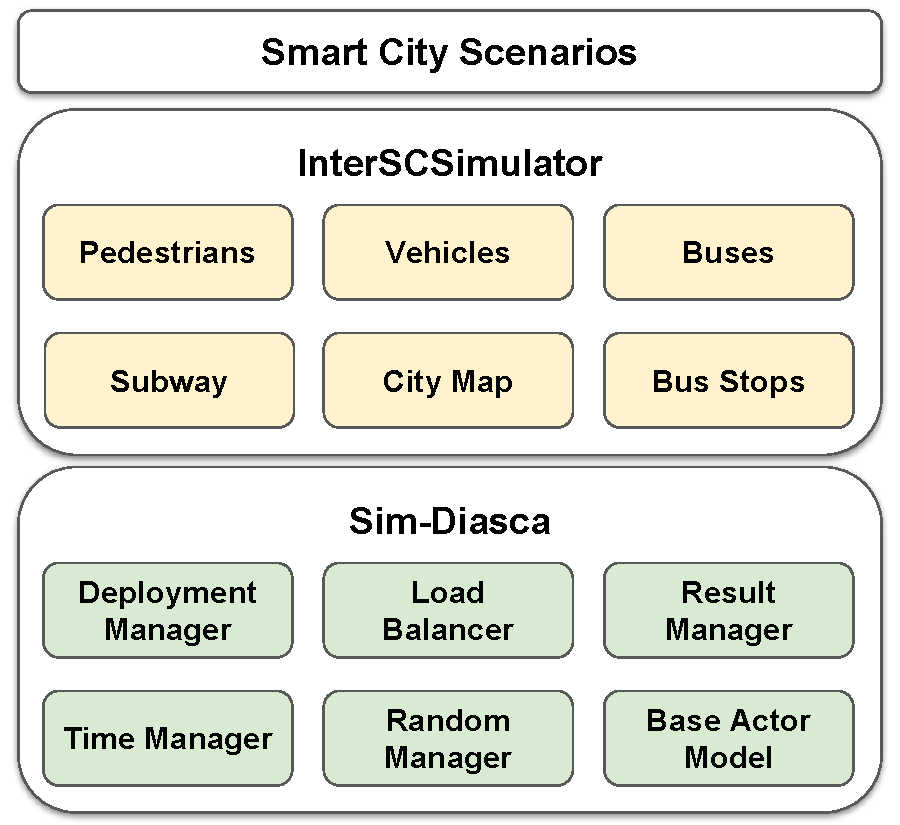
\includegraphics[width=0.9\textwidth]{figuras/chap-interscsimulator/Architecture.pdf}
\caption{InterSCSimulator Architecture}
\label{fig:arquitetura}
\end{figure}

Sim-Diasca main requirements are the simulation time management, the random number generation (allowing reproducibility), the synchronization of the actors to guarantee the simulation consistency and a basic actor model to facilitate the development of the simulation model. Besides, using the Erlang language, Sim-Diasca facilitates the communication among the actors, the parallelism, and distribution of the simulator, and fault tolerance.

The City Model is composed of the actors that are simulated in the Smart City scenarios. This layer is the central development of this research. The current version of the simulator provides the following actors: \textbf{Person} that represents a person traveling in the city, \textbf{Car}, when a person travels in a car, \textbf{Bus}, that represents the buses moving in the city and allow the boarding of passengers, \textbf{Subway} that simulates the subway network of the city, \textbf{Sensor} to reproduce Smart City sensors. Besides the actors, there are many other structures in the model, such as the city graph representation, an API to retrieve real-time simulation data, and a structure to save the simulation event log.

\section{Mobility Models}
\label{sub:modelo}

InterSCSimulator has many models to simulate the mobility of a city population, including a traffic model, which calculates the speed of the vehicles in the streets, a simple pedestrian model, and a model to simulates public transportation travels by subway or buses. A person can also make a trip using different travel modes, for example, the person starts walking to a subway station, then makes subway travel, and finally, get a bus to reach his destination. The next subsections describe the main models used by the simulator.

\subsection{Vehicles Simulation}

Car travels are composed of a sequence of links that the car will pass. To calculate the speed of the car in each link, the InterSCSimulator uses a mesoscopic traffic model. This type of model simulates each car individually. However, the speed of these vehicles is calculated using a density function relating to the capacity of the street and the number of vehicles on the street \citep{song2017gpusimulation}. The model implemented uses the following density function:

\[
v=v0*(( 1 - ( \frac{k}{k_{jam}} ) ^ \beta ) ) ^ \alpha
\]

Where:

\begin{itemize}

\item $v0$: the maximum speed of the street, used when the street is not congested.
\item k: the current street density.
\item kjam: the density when the street is congested.
\item $\alpha$ e $\beta$: Configurable parameters that are defined by the calibration of the model. We used the values used in the original paper $\alpha$=1.0 and $\beta$=0.05. 

\end{itemize}

This function is always used when a vehicle enters in an edge of the graph. To calculates its speed, it is verified the current density in the edge and using the function, the speed is calculated. With the speed and the length of the edge, it is possible to calculate the time that the will need to go through the edge. The time is calculated using the following function:

\[
time = \frac{edge\_length}{vehicle\_speed}
\]

In the function, \textbf{time} is the seconds that the car takes to go through the edge, \textbf{vehicle\_speed} is the value calculated by the traffic model and represents the speed (m/s) of the car in the street, and  \textbf{edge\_length} is the street length (m) that is available at OpenStreetMaps.


\subsection{Pedestrian Simulation}

Pedestrian simulation resembles the vehicle simulation. However, the speed calculus is straightforward. We used a normal distribution with mean 1.2 m/s, and a random speed calculated to the person. The function used to calculate the time that a person will take to go through an edge is the same used by the vehicles.

\subsection{Subway Simulation}

To simulate the subway system, InterSCSimulator has the subway graph of the simulated city, and it calculates the travel time of the subway travel by the number of stations that separate the origin and destination stations of the trip. Commonly, city documents with the subway system describe the travel duration between two following stations. Hence, we use a fixed time to calculate the travel time of the person in the subway system.

When an agent arrives at the origin subway stations, it sends a message to an Erlang process which simulates the subway system with its destination station. The Erlang process calculates the time that the agent will spend in the subway system, and then the person waits this time. After this interval, the agent is moved to the destination station and can finish its travel.

\subsection{Bus Trip Simulation}

The buses are simulated using the same traffic model used by the cars. The difference is that the buses pass in a sequence of links that represent bus stops. The people in the bus stop can board the bus if the line of the bus is the same that they are waiting.

The person can go walking or by car from its origin until a nearby bus stop. In the bus stop, the person waits for a bus of his desired line. When the bus arrives, the person boards the bus and moves using the same path and speed of the bus. When the bus comes at the destination bus stop, the person outboards the vehicle and the person finishes his travel.

The buses can have a maximum of 75 passengers, which is the limit of the city of S\~ao Paulo\footnote{http://goo.gl/B7NJbj}. 

\subsection{Multimodal Travels}

The simulator allows a sequence of travels using the same or different travel modes. To this, each person can have a series of trips and the destination of each travel is the origin of the next one. Each travel does not have any relation to the previous one. However, the final attributes of the journey such as total time traveled distance, and travel cost is the sum of all travels.

\section{Simulator Components}
\label{sub:components}

InterSCSimulator has three main components: \textbf{Scenario Definition} which read the input files and creates the simulation scenarios. \textbf{Simulator Engine} responsible for executing the algorithms and models of the simulation. \textbf{Events Manager} that receives all the events occurred in the simulation and saves in the trace file or send to the real-time API.

At the end of the simulation, there are other two components based on the result simulation: \textbf{Animated Visualization} which allows the graphic visualization of the events in the city graph and \textbf{Output Analyses} that using the output data perform statistical analyses using scripts R. Figure \ref{fig:simComponents} presents the simulator components, the interactions among them, and the simulator input and output files.

\begin{figure}[!htb]
\centering
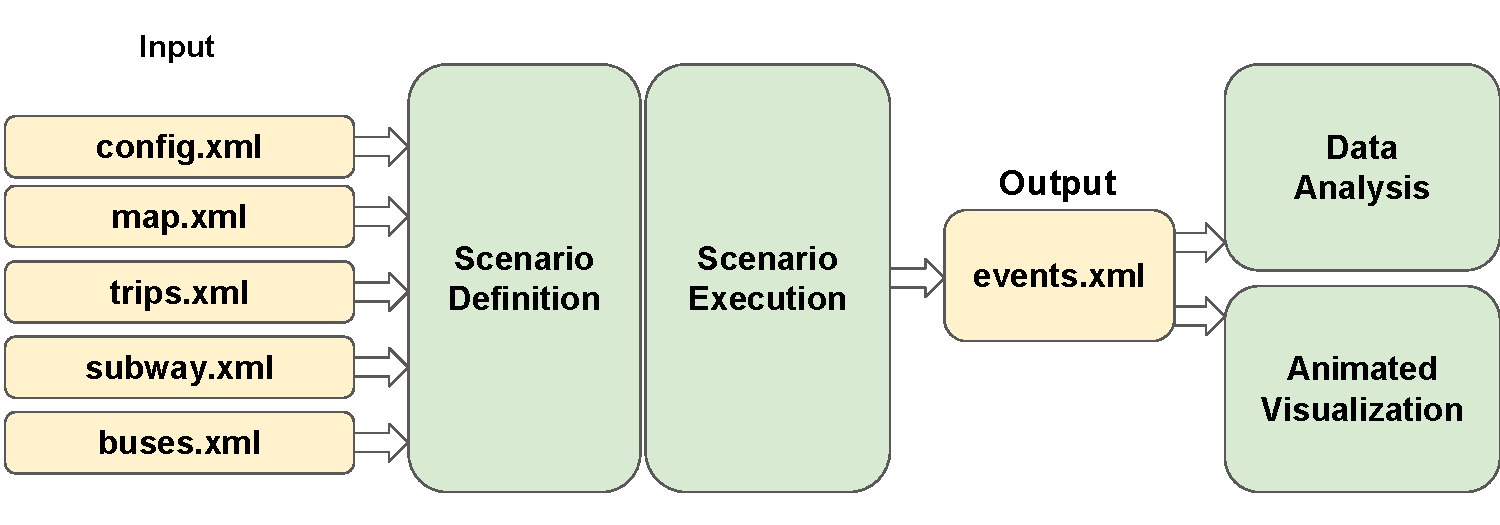
\includegraphics[width=1\textwidth]{figuras/chap-interscsimulator/components.pdf}
\caption{InterSCSimulator Components}
\label{fig:simComponents}
\end{figure}

The following sections will present each of the inputs, outputs, and components of the simulator.

\subsection{Inputs}

InterSCSimulator has three required XML files as input and other two optional files. The required files are:

\begin{itemize}

\item \textbf{config.xml} contains the path to the input and output files and the total simulation time.

\item \textbf{map.xml} has the digraph representing the road network of the simulated city. We used the map on the OpenStreetMap format in which the junctions are the vertices, and the streets are the links of the graph.

\item \textbf{trips.xml} defines the trips that must be simulated, each trip must determine its options such as origin, destination, start time, and travel mode.

\end{itemize}

The optional files are:

\begin{itemize}
    
\item \textbf{subway.xml} describes the city subway system as a graph which the stations are the vertices and the connection among the stations the edges.

\item \textbf{buses.xml} contains the bus lines of the city, including its name, interval, and bus stops sequences.

\end{itemize}

The map file is transformed in a digraph using the Digraph API of the Erlang language\footnote{Erlang Digraph API - \url{erlang.org/doc/man/digraph.html}}. Listing \ref{list:city} shows an example of a map used in the simulator.

\renewcommand{\thelstlisting}{\arabic{lstlisting}}
\lstset{language=XML}
\begin{lstlisting}[language=XML, caption=File describing the city road network, label=list:city, upquote=true]
<network>
 <nodes>
  <node id ="1" x="-46.65805" y="-23.58162" />
  <node id ="2" x="-46.65828" y="-23.58342" />
  <node id ="3" x="-46.65228" y="-23.59341" />
  <node id ="4" x="-46.63128" y="-23.51241" />
  <node id ="5" x="-46.59228" y="-23.54341" />
 </ nodes>
 <links>
  <link id="35985" from="1" to="2" length="100" freespeed="40" />
  <link id="35986" from="2" to="3" length="200" freespeed="40" />
  <link id="35987" from="3" to="1" length="80" freespeed="50" />
  <link id="35988" from="4" to="1" length="180" freespeed="50" />
  <link id="35989" from="1" to="5" length="30" freespeed="30" />
  <link id="35990" from="6" to="2" length="40" freespeed="50" />
  <link id="35991" from="7" to="2" length="50" freespeed="50" />
  <link id="35992" from="1" to="7" length="60" freespeed="40" />
  <link id="35988" from="3" to="6" length="180" freespeed="50" />
 </ links>
</network>
\end{lstlisting}

The map file has two section, the first describes the vertex of the graph, that are intersections among the cities roads. The vertex has three attributes, an Id, the latitude and the longitude. The second section contains all the edges of the graph, which represents a street stretch. The properties of the edges are its length, maximum speed, and capacity.

The trip file contains all the travels that must be simulated. Each travel has an origin and destination, the start time, and the travel model. A best path algorithm is used to define the travel path in the city graph. Listing  \ref{list:trips} presents an example of trips file with a set of travels.

\renewcommand{\thelstlisting}{\arabic{lstlisting}}
\lstset{language=XML}
\begin{lstlisting}[language=xml, caption=File containing the trips that will be simulated, label=list:trips, upquote=true]
<scsimulator_matrix>
 <trip origin="24751" dest="60613" start="2880" mode="car" />
 <trip origin="60613" dest="24791" start="6300" mode="car" />
 <trip origin="45110" dest="21990" start="1620" mode="car" />
 <trip origin="21090" dest="45110" start="6540" mode="car" />
 <trip origin="24751" dest="24650" start="3420" mode="car" />
 <trip origin="24650" dest="24751" start="5400" mode="car" />
 <trip origin="24751" dest="24650" start="6660" mode="car" />
 <trip origin="24650" dest="24751" start="8550" mode="walk" />
 <trip origin="24751" dest="24751" start="2370" mode="car" />
 <trip origin="24751" dest="24751" start="4440" mode="car" />
 <trip origin="24751" dest="60658" start="2880" mode="car" />
 <trip origin="60658" dest="24791" start="4320" mode="car" />
 <trip origin="24751" dest="41594" start="6840" mode="walk" />
 <trip origin="25822" dest="27925" start="7920" mode="car" />
 <trip origin="27925" dest="66111" start="5760" mode="car" />
 <trip origin="66111" dest="27925" start="6480" mode="car" />
 <trip origin="24751" dest="33026" start="4230" mode="car" />
</scsimulator_matrix>
\end{lstlisting}

It is also possible to simulate multimodal travels. For example, a person can walk until a bus stop, take a bus to a subway station, and then go walking from other metro station until its work. Listing \ref{list:multi_trips} presents examples of multimodal travels.

\renewcommand{\thelstlisting}{\arabic{lstlisting}}
\lstset{language=XML}
\begin{lstlisting}[language=xml, caption=Multi-Trip file, label=list:multi_trips, upquote=true]
<multi_trip name="1"  count="45" start="43201" mode="bus">
  <trip origin="25298" dest="17409" mode="walk"/>
  <trip origin="17409" dest="11072" line="8020-10-0" mode="bus"/>
  <trip origin="11072" dest="30469" line="675N-10-0" mode="bus"/>
  <trip origin="30469" dest="30469" mode="walk"/>
</multi_trip>
<multi_trip name="3" count="82" start="45001" mode="metro">
  <trip origin="41972" dest="44116" mode="walk"/>
  <trip origin="44116" dest="25781" mode="metro"/>
  <trip origin="25781" dest="30165" mode="walk"/>
</multi_trip>
<multi_trip name="4" count="37" start="61201" mode="metro">
  <trip origin="31468" dest="29513" mode="walk"/>
  <trip origin="29513" dest="28267" mode="metro"/>
  <trip origin="28267" dest="60642" mode="walk"/>
</multi_trip>
\end{lstlisting}


The Config file defines some parameters to the simulator such as the total time of the simulation, the path to the input and output files and what analyses will be executed in the final of the simulation. Listing \ref{list:config} presents an example of this file.

\renewcommand{\thelstlisting}{\arabic{lstlisting}}
\lstset{language=XML}
\begin{lstlisting}[language=xml, caption=File with the simulator configurations, label=list:config, upquote=true]
<scsimulator_config>
    <config trip_file="path_to_trip_file" />
    <config map_file="path_to_map_file" />
    <config bus_file="path_to_bus_file" />
    <config subway_file="path_to_subway_file" />
    <config simulation_time="86400" />
    <outputs>
        <chart name="mostUsedRoads" />
        <chart name="meanVelocityHour" />
        <chart name="tripTimeByMode" />
    </outputs>
</scsimulator_config>
\end{lstlisting}

The subway file defines the subway graph of the simulated city which has two sections. The first describes the subway stations and the second the connections among the stations. Listing \ref{list:subway} presents an example of the definition of a subway line in the input file.

\renewcommand{\thelstlisting}{\arabic{lstlisting}}
\lstset{language=XML}
\begin{lstlisting}[language=xml, caption=File with the definition of the city subway graph, label=list:subway, upquote=true]
<metro>
  <stations>
    <station name="Vila Prudente" idNode="252018921" />
    <station name="Tamanduatei" idNode="674412889" />
    <station name="Sacoma" idNode="2533391001" />
    <station name="Alto Do Ipiranga" idNode="4443113954" />
    <station name="Santos-imigrantes" idNode="1484829870" />
    <station name="Chacara Klabin" idNode="922094745" />
    <station name="Ana Rosa" idNode="467744160" />
    <station name="Paraiso" idNode="459347687" />
    <station name="Brigadeiro" idNode="856727276" />
    <station name="Trianon-masp" idNode="2021000708" />
    <station name="Consolacaoo" idNode="1819616337" />
    <station name="Clinicas" idNode="1952545109" />
    <station name="Sumare" idNode="466808387" />
    <station name="Vila Madalena" idNode="1415720983" />
  </stations>

  <links>
    <link idOrigin="674412889" idDestination="252018921" />
    <link idOrigin="2533391001" idDestination="674412889" />
    <link idOrigin="4443113954" idDestination="2533391001" />
    <link idOrigin="1484829870" idDestination="4443113954" />
    <link idOrigin="922094745" idDestination="1484829870" />
    <link idOrigin="467744160" idDestination="922094745" />
    <link idOrigin="459347687" idDestination="467744160" />
    <link idOrigin="856727276" idDestination="459347687" />
    <link idOrigin="2021000708" idDestination="856727276" />
    <link idOrigin="1819616337" idDestination="2021000708" />
    <link idOrigin="1952545109" idDestination="1819616337" />
    <link idOrigin="466808387" idDestination="1952545109" />
    <link idOrigin="1415720983" idDestination="466808387" />
  </links>
</metro>
\end{lstlisting}

The buses file defines the bus lines in the simulated city. Each bus line has the following attributes: \textbf{Id} is the name of the line; \textbf{interval} is the dispatch time interval of the buses of the line; \textbf{start\_time} is the bus first dispatch time of the day; \textbf{stops} is the list of bus stops whose the bus must stop to load or unload passengers. Listing \ref{list:buses} presents an example of the definition of bus lines in the simulator.

\renewcommand{\thelstlisting}{\arabic{lstlisting}}
\lstset{language=XML}
\begin{lstlisting}[language=xml, caption=Definition of the city buses, label=list:buses, upquote=true]

<scsimulator_buses>
    <bus id="1016-10-0" interval="1800" start_time="18000" stops="507969889,2390204059,507969889,1400446171" />
    <bus id="1016-10-1" interval="1800" start_time="18000" stops="2396517544,163220296,2390192810,2390192798
    " />
    <bus id="1017-10-0" interval="1800" start_time="18000" stops="832264854,1758396031,832264854,2448473366" />
    <bus id="1017-10-1" interval="1800" start_time="18000" stops="934050061,2109902387,2448473366,832264854" />
    <bus id="1018-10-0" interval="1800" start_time="18000" stops="2116463109,2390204059,507969889,2390204059" />
    <bus id="1018-10-1" interval="1800" start_time="18000" stops="2520196336,507969946,410243261,410243260" />
    <bus id="1024-10-0" interval="1800" start_time="18000" stops="934050061,1430544803,917144410,1430544803,917144410" />
    <bus id="1025-10-0" interval="1800" start_time="18000" stops="934050061,1430544803,917144410,1430544803" />
    <bus id="106A-10-0" interval="1800" start_time="18000" stops="2390339037,1709028082,185795118,929591881" />
</scsimulator_buses>

\end{lstlisting}

\subsection{Scenario Definition}

The Scenario Definition component parses the input file and creates the simulation scenario. Additionally, it creates all the management Erlang actors and sets all the parameters of the simulation such as the simulation time and the output path. The most critical actors created in this phase are the \textbf{travel manager}, which generates the people actors during the simulation, \textbf{subway manager} which represents the subway system of the city, \textbf{city manager} which describes the road network of the town, and the \textbf{output manager} which saves all the simulation events to the log file.

In this phase are also calculated the best path to all the car and pedestrian travels. It is made before the simulation because it is a costly operation and if it was executed during the simulation could waste a lot of processing time.

\subsection{Simulation Execution}
\label{sub:execucao}

In the execution of the simulator, the most important actions are the movement of people on foot, by car, or by public transportation. Each person of the simulation make an action (or event) and then schedules its next movement. The movement depends on the transportation modal of the person. In the following, we describe the main events that a person can execute during the simulation.

\begin{itemize}

\item \textbf{Start Travel: } When the simulation time is equal to the start time of the travel configuration, an agent is created to simulate that travel. Independently of the transportation mode. In this event, the agent goes to the first link of its path.

\item \textbf{Move: } If an agent is moving on foot or car when it leaves a link and enters in another one, it is generated a move event. In this event, it is calculated the time that the agent will require to pass through the link. Walks and car travels are a succession of move events.

\item \textbf{Move Bus:} When an agent arrives at a bus station, it waits until a bus of the line that it is waiting arrives. When the bus arrives, the agent enters the bus and generates a move bus event. After, the agent moves with the bus until its bus stop destination.

\item \textbf{Move Subway: } If an agent will travel by subway when it arrives at the subway station, it informs the SubwayManager their origin and destination stations. The SubwayManager calculates the time in which the agent will spend in the subway system and notifies the agent. 

\item \textbf{Arrival: } When the agent arrives at its final destination, it creates an arrival event that saves the attributes of the travel in the output file such as the total time, distance, and cost. After this event, the agent is removed from the simulation.

\end{itemize}

The execution of the events is based on the models described in Section \ref{sub:modelo}. All the events are saved on the simulator output file in chronological order and have common attributes such as simulation tick, link, type, and id of the agent which executed the event.

\subsection{Outputs}
\label{sub:saida}

As output, InterSCSimulator generates an XML or CSV file with all the events occurred during the simulation. The possible events are the ones described in the previous section. Listing \ref{list:csv_output} presents a stretch of the file with a simulation output.

\lstset{language=XML}
\begin{lstlisting}[caption=CSV output file, label=list:csv_output]
192;arrival;8062_65;102388;126;616
200;arrival;8062_74;102388;126;616
228;arrival;8062_38;102388;126;616
235;arrival;8000_50;106030;186;1542
244;arrival;8062_37;102388;126;616
257;arrival;49_10;48743;157;807
257;arrival;49_17;48743;157;807
258;arrival;8062_20;102388;126;616
259;arrival;2280_15;13694;91;407
269;arrival;3241_72;42753;144;1668
\end{lstlisting}

In Listing \ref{list:csv_output} the first four elements are common to all events which are the simulation tick, the event, the agent id, and the link where the event occurred. Depending on the event, it could have more elements, such as the arrival event that also saves the total distance and the total time of the travel.

To generate the XML file, we used the MATSim format, allowing the usage of OTFVis\footnote{OTFVis --- \url{matsim.org/docs/extensions/otfvis}}, a tool to generate an animated visualization of the simulation. Listing \ref{list:xml_output} presents a stretch of the file with the XML output.

\lstset{language=XML}
\begin{lstlisting}[language=xml, caption=XML output file, label=list:xml_output]
<events version="1.0">
  <event time="28" type="departure" person="p1" link="1425"  />
  <event time="28" type="entered link" person="p1" link="15" vehicle="car1" />
  <event time="32" type="entered link" person="p1" link="13" vehicle="car1" />
  <event time="54" type="entered link" person="p1" link="16" vehicle="car1" />
  <event time="62" type="entered link" person="p1" link="36" vehicle="car1" />
  <event time="78" type="entered link" person="p1" link="21" vehicle="car1" />
  <event time="96" type="entered link" person="p1" link="42" vehicle="car1" />
  <event time="110" type="entered link" person="p1" link="57" vehicle="car1" />
  <event time="114" type="entered link" person="p1" link="72" vehicle="car1" />
  <event time="118" type="entered link" person="p1" link="67" vehicle="car1" />
  <event time="125" type="arrival" person="p1" vehicle="car1" link="88" trip_time="191" distance="2634" />
</events>
\end{lstlisting}


\subsection{Simulation Visualization}

Using the output data, it is possible to generate different visualizations of the simulation results. For example, it is possible to create an animated visualization of the simulation events. This visualization shows the city road network and the cars moving in the city. Figure \ref{fig:sao_paulo_map} presents the visualization of one simulation in the city of S\~ao Paulo. Each green point in the figure is a car moving in the city graph.

\begin{figure}[!htb]
\centering
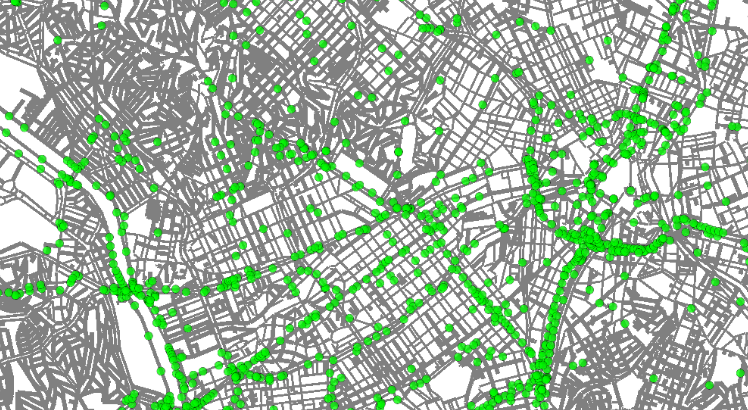
\includegraphics[width=0.9\textwidth]{figuras/chap-interscsimulator/mapa.png}
\caption{S\~ao Paulo Simulation}
\label{fig:sao_paulo_map}
\end{figure}

To show that InterSCSimulator works in any map generated from the OSM, we also made a simple simulation using the map of New York. Figure \ref{fig:newYork} presents the visualization of this simulation using OTFVis.

\begin{figure}[!htb]
\centering
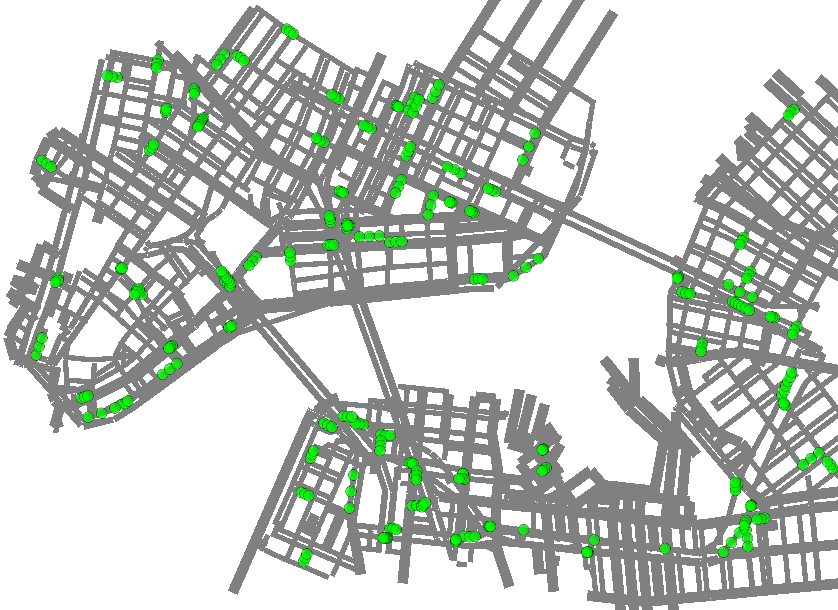
\includegraphics[width=0.7\textwidth]{figuras/mapaNy.png}
\caption{New York Simulation}
\label{fig:newYork}
\end{figure}

Despite that OTFVis is capable of simulating large simulations with more than 50 thousand actors at the same time, it does not have the same scalability as InterSCSimulator. Therefore, it is necessary more research allow the visualization of a very-large simulation in a large graph such as S\~ao Paulo road network.

Besides the animated visualization, we also created a component that executes scripts written in R language to perform statistical analyses with the output data of the simulator. These scripts generate a series of charts such as the mean speed of the cars during the simulation time, the most used links in the simulation, and the mean time of the travels by the transportation mode. Figure \ref{fig:chart_example} shows a chart generated by an R script which shows the 10 most used links during the simulation.

\begin{figure}[!htb]
\centering
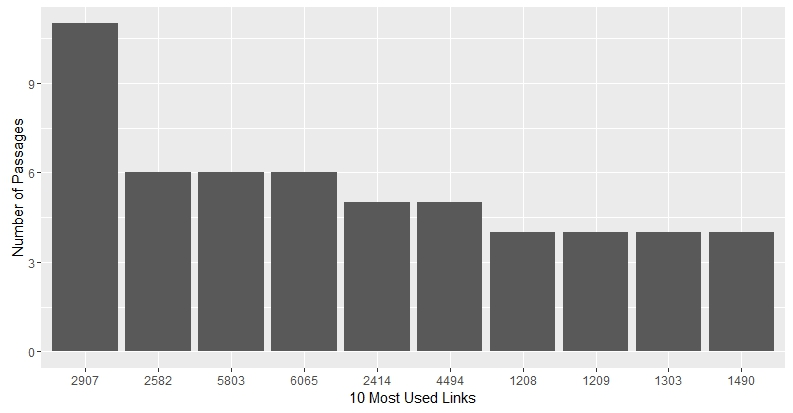
\includegraphics[width=0.8\textwidth]{figuras/chart_top_ten.jpeg}
\caption{Most used links in the simulation}
\label{fig:chart_example}
\end{figure}

Figure \ref{fig:chart_example2} presents another example of a chart generated using the simulation output data. This chart presents the mean travel time by the different type of travels such as agents going to work, to home, or going to hospitals.

\begin{figure}[!htb]
\centering
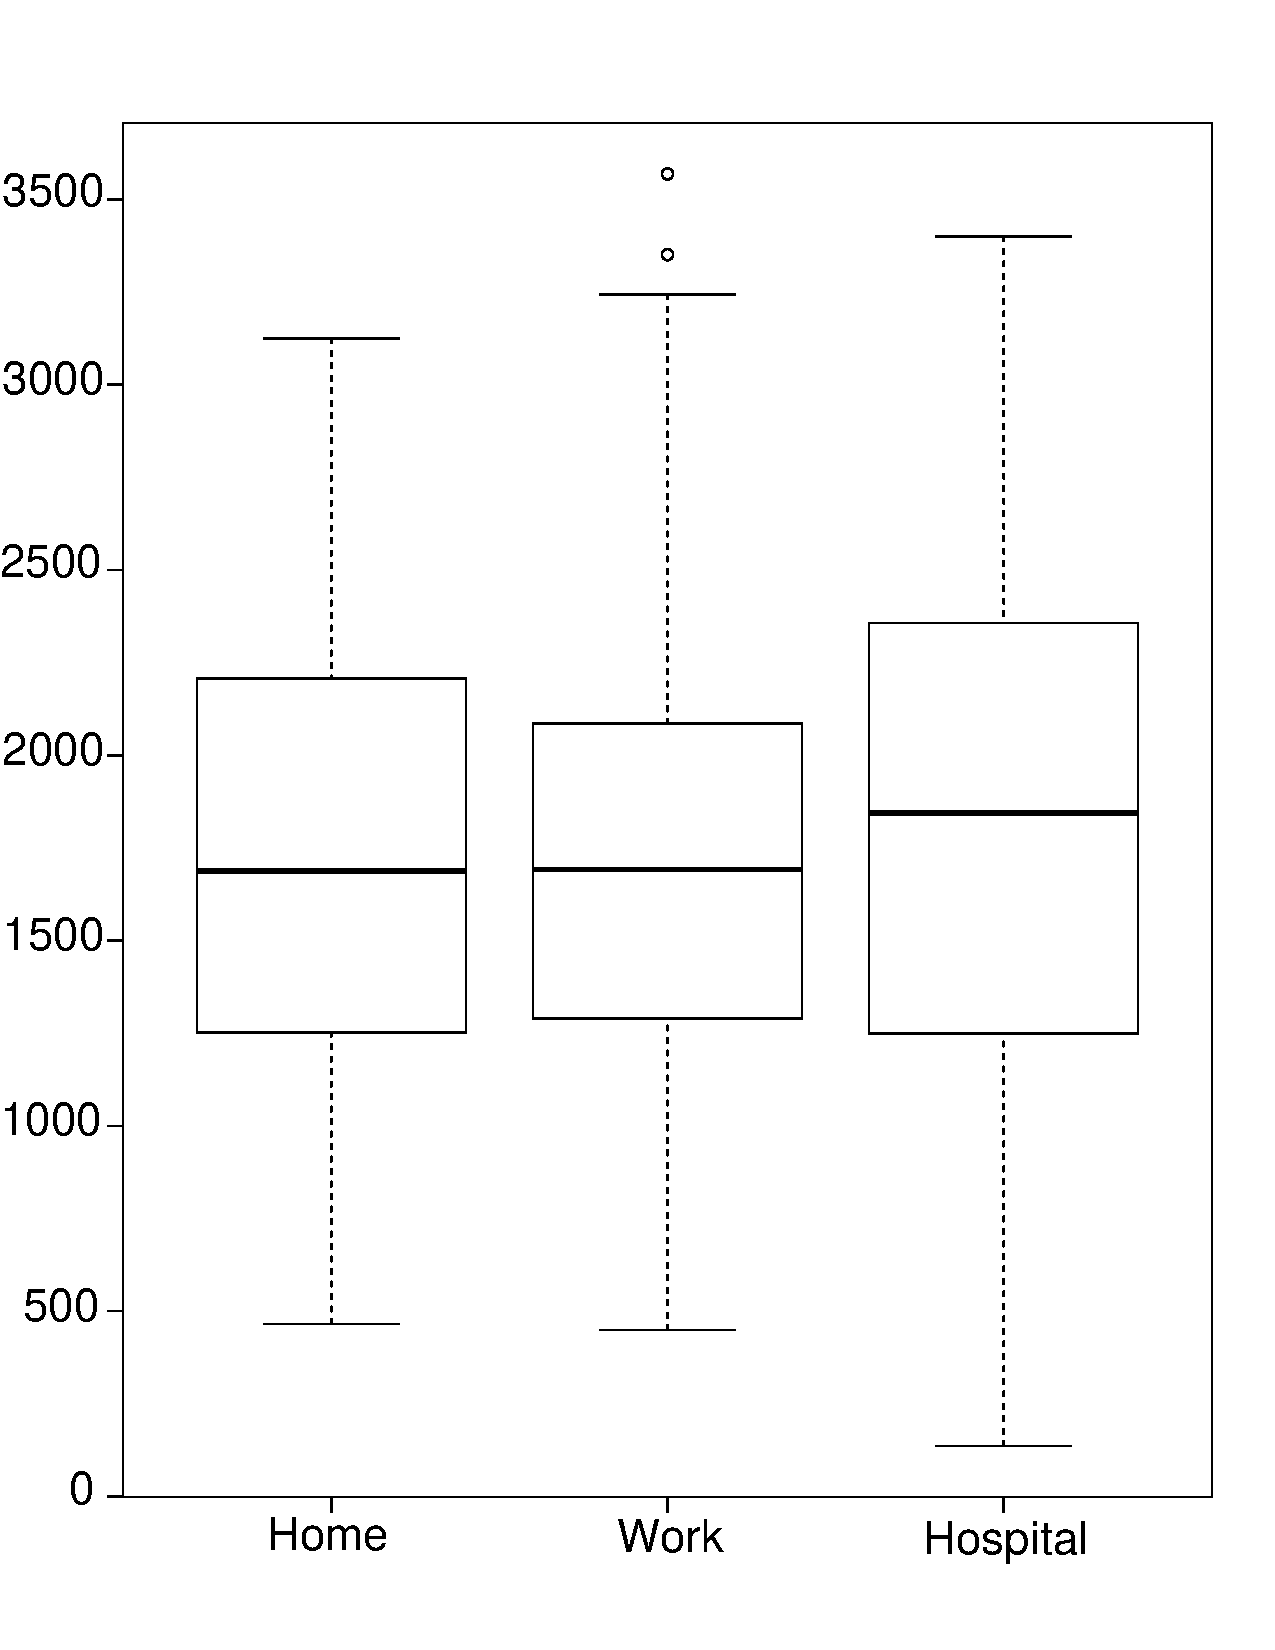
\includegraphics[width=0.6\textwidth]{figuras/mode_trip.pdf}
\caption{Mean travel time by travel type}
\label{fig:chart_example2}
\end{figure}


\section{Other Simulations}
\label{sec:outros}

Besides the models described in this Chapter, we also implemented other components of Smart Cities applications such as:

\begin{itemize}

    \item \textbf{Parking Spots:} We also developed the simulation of parking spots, which allow the configuration of a car travel that the person must find a free place to park the car. The idea of this simulation was to verify the impact in the city traffic of using a Smart Parking application, helping drivers to find the closest free parking spot.
 
    \item \textbf{Sensors:} The simulator enables the definition of a set of sensors which generates data in a time interval. These actors allow the simulation of different type of sensors such as air pollution, noise, traffic counters, and humidity. The simulation of sensors enables tests and experiments of Smart City applications and platforms.
    
    \item \textbf{Locations:} It is possible to simulate locations in the simulator. These locations can generate random travels in the city using a statistical distribution. The idea of this model is to reproduce places in the city that can spawn traffic such as stadiums, shopping centers, and large condominiums.
    
    \item \textbf{Events:} The simulator allows the simulation of events in the city streets such as an accident that interferes in the flow of vehicles or streets closure in a weekend for leisure. The idea of simulating events is to evaluate how an event impacts the traffic of the city.
    
\end{itemize}


\section{Simulator Architecture Evolution}
\label{sec:evolucao}

Achieve the current scalability of the simulator was a big challenge. We had to develop different algorithms and use many data structures during the simulator implementation. This section presents the most significant modifications to the simulator architecture to improve the execution time and memory usage. The most significant improvements were in the city graph representation and the actor's creation.

\subsection{City Graph Representation}

To manipulate the city graph, we use the Erlang Digraph API\footnote{Digraph API -- http://erlang.org/doc/man/digraph.html} which facilitates a lot the creation of graphs and the execution of many algorithms such as the best path and minimal spanning tree.

In the first version of the simulator, we maintained the city graph in a unique Erlang actor. When a car entered a link, it must send a message to the graph actor and waits for the execution of the traffic model to get the time that it took to go through the street. This model worked but had a very high execution time, because this central actor was a bottleneck in the simulator architecture. We did not execute scalability tests in this version because we could simulate at most 50,000 agents in this version of the simulator.

The first solution to this problem was creating an independent actor to each vertex in the graph. In the second version, each actor had the id of the vertex and a dictionary\footnote{Erlang Dictionary -- http://erlang.org/doc/man/dict.html} with all the links to the adjacent vertex. This dictionary stored the attributes of the link such as its length, capacity, and the current number of cars in the link. This version increased a lot the use of memory to store the city graph but lowered the execution time of the simulator. With this version, it was possible to execute simulations with more than 4 million actors in a single simulation. Figure \ref{fig:execution_time} shows the execution time of this version of the simulator using a S\~ao Paulo scenario with 1, 2, 3, and 4 million cars.

Although the second version of the simulator improved a lot the simulator execution time, the architecture of the simulator with an Erlang actor to each vertex of the graph was using much memory and when the traffic was very congested, a number of vertex, mainly the ones that represented big avenues in the city, the execution time of the simulation increased a lot. To solve this problem, we used the Erlang ETS (Erlang Term Storage) Tables \citep{aronis2017shared}.

The ETS Table is an in-memory store object available in the Erlang Virtual Machine. An ETS Table is capable of storing large amounts of objects with a constant time data access. All the Erlang actors can access and update an ETS table that is running in the Erlang VM. To avoid concurrency problems, the ETS API provides a series of atomic operations such as increment, decrements, exclusion of lists, and value update.

The third, and current, version of the simulator uses an ETS table to store the city graph. In this version, the digraph API is used only to calculate the travel paths. The models use the ETS that has all the vertex and links of the graph. Using the ETS there is no bottleneck in the simulator, the only problem that can occur is if two or more vehicles try to enter in the same link at the same moment. If this occurs, the cars will have to wait for the update in the ETS table from the other cars. The use of ETS table improved the execution time of the simulator almost three times. Figure \ref{fig:execution_time} shows the execution time of this version of the simulator using the same scenarios of the previous Figure.

\begin{figure}[!htb]
\centering
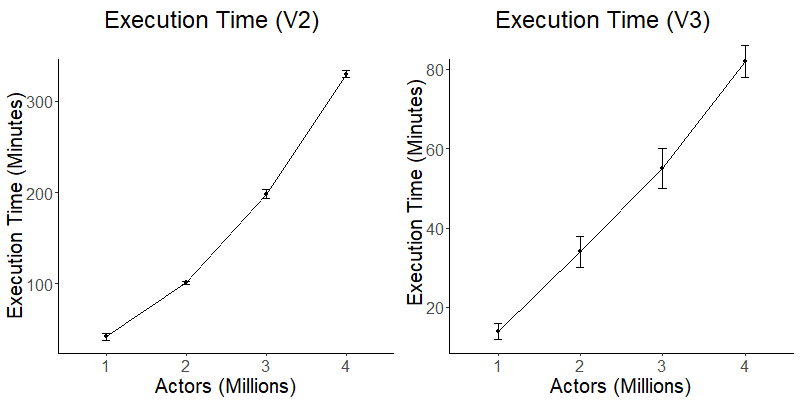
\includegraphics[width=1.0\textwidth]{figuras/chap-interscsimulator/execution_time.png}
\caption{Execution Time of InterSCSimulator V2 and V3 (ATUALIZAR PARA OS GRÁFICOS DA NOVA VERSÂO)}
\label{fig:execution_time}
\end{figure}

\subsection{Actors Creation}

In the InterSCSimulator, an Erlang actor performs each simulated travel. Therefore, if a simulation has 10 million travels, 10 million Erlang actors are created during the simulation. In the first version of the simulator, all the actors were created during the simulation. It was not a problem because the simulator maximum scalability was 50 thousand actors.

However, in the second version of the simulator, the scale increased a lot and the creation of the actors was a bottleneck in the simulation and we found a bug in the Sim-Diasca simulator that made the creation of actor very slow. To minimize this problem, we decided to create all the actors before the simulation start. This approach solved the scalability problem but increased the memory used by the simulator. Figure \ref{fig:memory_used} shows the memory used to execute the simulations in this version of the simulator.

In the third version, the Sim-Diasca developers solved the problem in the actor creation and released a new version of the simulator. Therefore, we could return to the first approach and create the actors during the simulation. Along with other improvements in the simulator, including the ETS tables, the third version of the simulator uses almost five times less memory to execute. Figure \ref{fig:memory_used} shows the memory used to execute the simulations in this version of the simulator.

\begin{figure}[!htb]
\centering
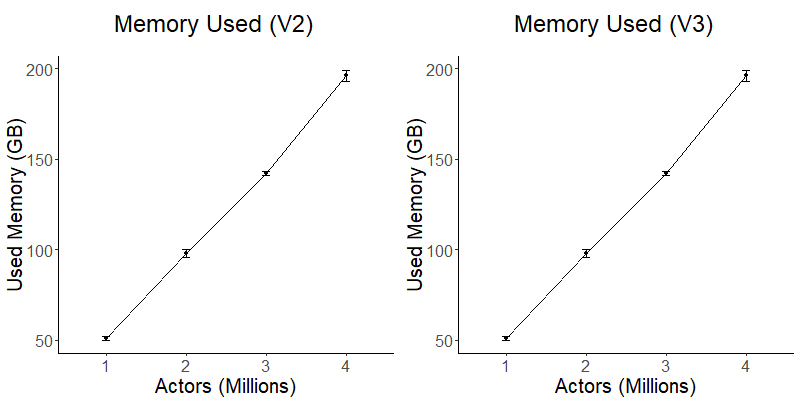
\includegraphics[width=1.0\textwidth]{figuras/chap-interscsimulator/memory_used.png}
\caption{Memory Used in InterSCSimulator V2 and V3(ATUALIZAR PARA OS GRÁFICOS DA NOVA VERSÂO)}
\label{fig:memory_used}
\end{figure}
\par


\chapter{Case Study: S\~ao Paulo Simulation}
\label{cap:sao_paulo}

This chapter presents the simulation of the city of S\~ao Paulo as a use case of InterSCSimulator. Also, we validated and verified the models described in Chapter \ref{cap:interscsimulator} using this scenario. The simulation validation and verification are critical to demonstrating that the models are working and producing useful results. This simulation is also the basis for the scalability analyzes presented in Chapter \ref{cap:avaliacao}.

\section{Input Data}

We based our simulation in real data collected from different sources. The databases considered in this simulation are:

\begin{itemize}

\item Origin-Destination (OD) Matrix derived from a survey conducted by the city subway company for the year 2012\footnote{Origin-Destination Survey - \url{http://goo.gl/Te2SX7}}

\item Map of the city based on OpenStreetMap \footnote{OpenStreetMap - https://www.openstreetmap.org}

\item Buses lines and stops of the city provided by the Municipal Transportation Secretary

\item Subway network of the city provided by the Metr\^o Company

\end{itemize}

\subsection{Origin-Destination Survey}

The OD survey of the city has more than 60 thousand registers. Each register contains information about travel of one person from an origin to a destination which are different places in the city such as houses, workplaces, and schools. Besides the origin and destination, there are other valuable data about the travels such as the start time, expected arrival time, and transportation mode. The survey has information about bus, cars, rides, bicycle, suburban trains, and subway travels.

Other fundamental information to the simulator is an extrapolation factor which estimates the number of people that make similar trips to the person of the OD register. We use this data to simulate the entire city population randomly positioning the people of the extrapolation factor close to the original position of the OD. With this information, there are more than 20 million travels and 11 million people in the OD, what is very close to the entire population of the city of S\~ao Paulo. 

Figure \ref{fig:travel_count_mode} presents the number of travels in the OD survey. There are 5.058.002 travels by car, 4.029.546 travels by buses, 6.287.487 travels on foot, and 3.030.809 travels by subway or suburban train. The figure shows that most of the city population makes their trips walking or using public transportation, especially buses. However, there are also a huge number of cars in the city streets. The OD survey has data about other transportation modes such as cars passengers, bicycles, taxis, and school buses. We did not consider these modes because some of them do not impact the traffic such as car passengers or we do not have real data to make useful simulation such as bicycles, taxis, and school buses.

\begin{figure}[!htb]
\centering
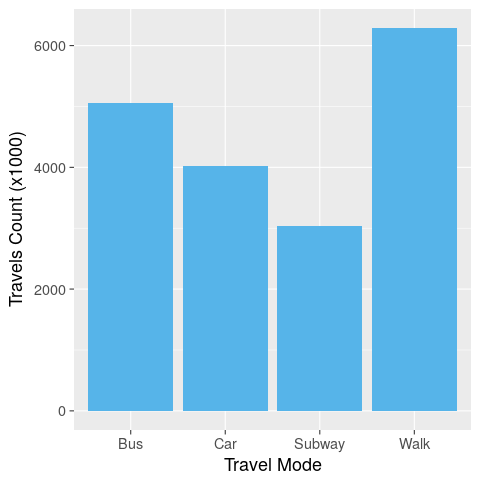
\includegraphics[width=0.6\textwidth]{figuras/chap-sp/travel_count.png}
\caption{Total Number of Trips by Transportation Mode}
\label{fig:travel_count_mode}
\end{figure}

Another essential information to the simulation is the time when each person starts his travel. Figure \ref{fig:travel_count_mode_and_hour} presents the travels start time grouped by the start time using 1-hour intervals. This chart shows that there is a considerable variation in the number of travels during the day. Most of the travels are during the peak hours (from 6 to 9 am and from 5 to 8 pm) and at the lunchtime. However, most of the travels during lunch time are on foot or by subway and are small travels. Probably they are performed by people going from their work to restaurants or home to lunch.

\begin{figure}[!htb]
\centering
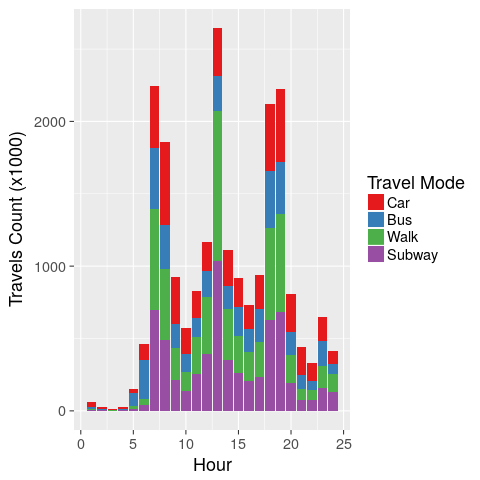
\includegraphics[width=0.6\textwidth]{figuras/chap-sp/mode.png}
\caption{Number of Trips by Transportation Mode and by Hour}
\label{fig:travel_count_mode_and_hour}
\end{figure}

Another relevant information is that the OD survey has only the primary transportation mode of the commuters. Hence, it is possible that many people use more than one transportation mode during one travel. For example, in S\~ao Paulo it is common to have buses from a neighborhood that go to subway stations, where most of the people take the subway to arrive at the downtown. Finally, the OD has the expected travel time of the commuters. We used this information to verify if the used mobility models are generating reasonable results.

A problem with the OD survey is that it is updated every five years. Of course, there are many changes in the city mobility in this interval. However, even with this problem, the OD survey is the most representative data about S\~ao Paulo mobility patterns.

\subsection{City Map}

We used the OpenStreetMap to generate the graph of the city. This graph has approximately 50 thousand nodes and 120 thousand links and covers most of the streets and roads of S\~ao Paulo and some parts of its metropolitan area. In the graph, the links represent stretches of the streets and the nodes the intersections. All the nodes in the graph have a unique id and their latitude/longitude. The links have the start and end node, the maximum speed, the length, the type, and the capacity of the street. With this graph, we can implement all the models described in Section \ref{sub:modelo}.

\subsection{Bus Lines and Stops}

To simulate the buses lines and stops of S\~ao Paulo, we used the data from the city transportation secretariat (SPTrans). They provided a spreadsheet with all the lines of the city with information about them such as the code, the stops, the start time, and the average interval of the buses along the day.

There are 2,347 lines in the city, and they have different characteristics. For example, some lines run only on weekends and lines that work just for a few hours, mainly in the peak hour. The numbers of stops can also vary a lot from line to line, on average each bus makes 43 stops in its route. However, there are buses with just four stops and others with 144 stops. Regarding the stops, S\~ao Paulo has 19,144 bus stops. As about the buses, there is a significant variance about the stops in the city. In average, five buses pass through each stop in the city. However, there are stops with just 1 line and others with 62 lines.

\subsection{Subway and Suburban Trains Network}

To simulate the subway and train system of S\~ao Paulo we created a digraph using the data about the lines of the city. Although different companies manage the train and the subway system (CPTM and Metrô), both systems are integrated and have the same cost to the users. The subway system has six lines, 79 stations, and an extension of almost 90 kilometers. The train network has seven lines, 90 stations, and an extension of more than 270 kilometers. Together, the two systems have more than 4 million users per day. 

\section{Simulation Execution}

Based on the data described in the last section, we created all the input files of InterSCSimulator and simulated an entire day in the city. The simulation was executed in a machine on the Google Cloud Environment with a memory of 160 GB and 16 cores. The simulation took approximately 7 hours to execute and at the peak used 138 GB of memory. The output file generated by the simulation has more than 17 million travels and occupy 2 GB of the disk.

\section{Validation and Verification}

According to Sargent \citep{sargent2013verification} to confirm if a simulator is generating useful results, it is essential to validate and verify the simulator output. The validation consists in analyzing if the models and data structures are working and generating the expected outputs. The verification compares the simulation results with the real system and the analyzed variables must be equal or very close in both cases. To validate the models we made several analyzes in the results of the simulator and to verify the simulation models we compared the real travel time of the OD survey with the simulated travel time. 

\subsection{Validation}

The output of the simulator is a mobility trace with all the events that occurred in the simulation. To analyze the travel times, we filtered just the arrival events which occur when a commuter arrives at his destination. In this event, we save the total travel time and distance. With this data, we made analyzes about the mobility patterns in the city. For example, to show the concentration of people and vehicles, we generated a heat map with the agents in S\~ao Paulo downtown. Figure \ref{fig:heat_map} shows the people and vehicles in the morning peak hour, between 8 and 8:10. The Figure presents a significant concentration of vehicles in important avenues of the city such as 23 de Maio and Radial Leste which are known for their great congestion.

\begin{figure}[!htb]
\centering
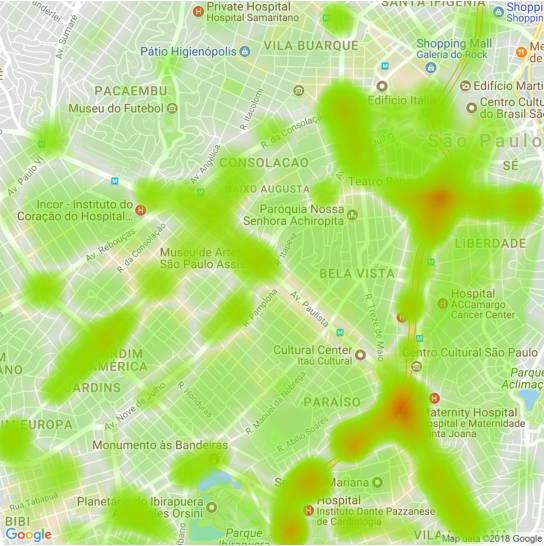
\includegraphics[width=0.8\textwidth]{figuras/chap-sp/mapa_calor.pdf}
\caption{Heat map of the simulated travels}
\label{fig:heat_map}
\end{figure}

\subsubsection{Vehicles Travels}

Figure \ref{fig:travel_time2} shows the analyzes to car travels with the mean travel time, distance, and speed of the vehicles depending on the arrival time of their arrival time. The last chart shows the total number of vehicles that finished a trip for each hour of the simulation.

\begin{figure}[!htb]
\centering
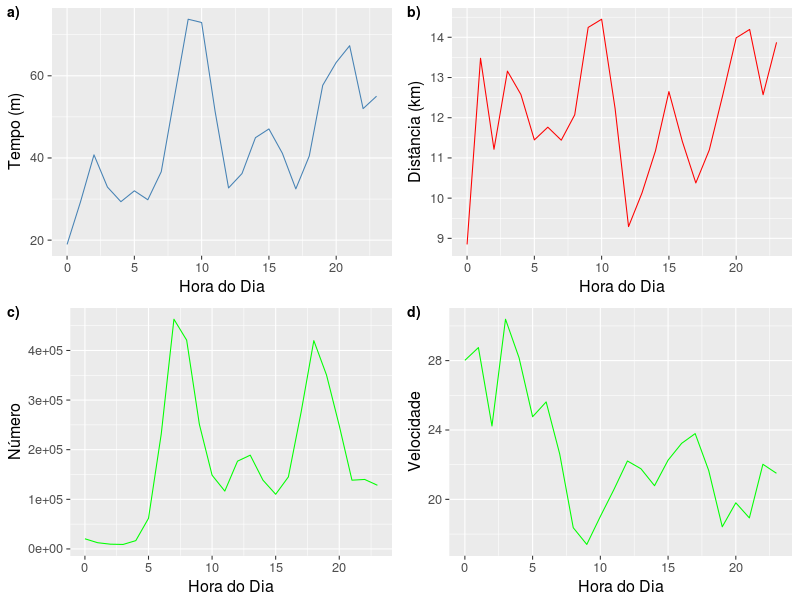
\includegraphics[width=1\textwidth]{figuras/chap-sp/time_distance_car.png}
\caption{Analyzes of the car travels}
\label{fig:travel_time2}
\end{figure}

The charts show that on average the travels are much slower in the peak hours than during the rest of the day. It is mainly due to the decrease in the average speed of the vehicles caused by the massive amount of vehicles that are moving in the city. It is also possible to verify that the distance is not very important in the travel time, the average distance of the travels varies from 10 km to 14 km during the day.

Figure \ref{fig:scatter_car} presents the correlation of time, distance, the hour of the day, and the speed of car travels. The Figure shows that some variables are very correlated such as time and distance and speed and time. Otherwise, there is no visible correlation between the distance and hour of the day and distance and speed.

\begin{figure}[!htb]
\centering
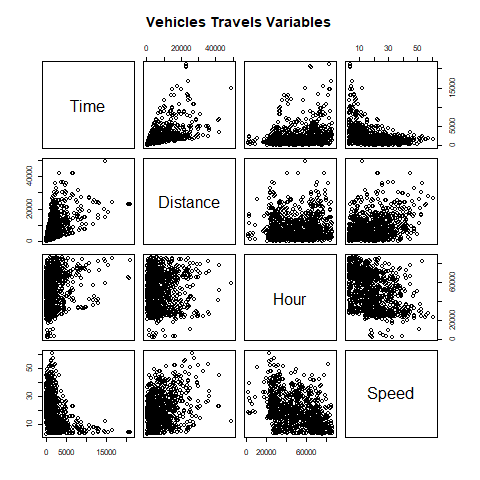
\includegraphics[width=0.8\textwidth]{figuras/chap-sp/scatter_car.png}
\caption{Correlation among Car travels variables}
\label{fig:scatter_car}
\end{figure}

\subsubsection{Subway Travels}

Figure \ref{fig:scatter_subway} presents the correlation of time, the hour of the day, and the number of stations on subway travels. As the chart shows, the number of stations define the inferior limit of the travel time. However, a significant part of the subway travel uses another transportation mode such as buses or walking. The chart also shows that there is a higher number of travels during the peaks hours, in the morning, at the lunchtime, and at the final of the afternoon.

Also, the chart shows that are a small number of travels in the very beginning of the day because the subway system of S\~ao Paulo works until approximately 00:30. The last train of almost all lines depart at midnight, and each station closes after this train leaves. The system opens at 04:40 every day. 

\begin{figure}[!htb]
\centering
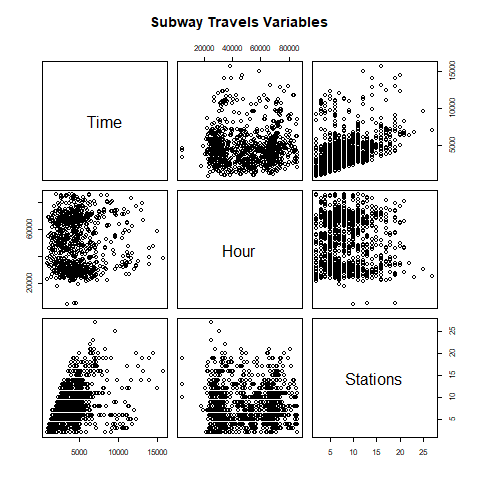
\includegraphics[width=0.8\textwidth]{figuras/chap-sp/scatter_subway.png}
\caption{Correlation among Subway travels variables}
\label{fig:scatter_subway}
\end{figure}

A limitation of our work is that in the peak hours it is probably that a user will take some time waiting for a train in a station, it occurs because the trains already arrive full or there is a massive queue to enters the train. We do not model this time wasted to get the next train yet. However, it is possible to create a model that calculates the time to enter a train based on the number of people that is in the stations.

\subsubsection{Pedestrian Travels}

Figure \ref{fig:scatter_walk} presents the correlation of time, the hour of the day, and the distance of pedestrian travels. The Figure shows that there is a linear correlation between the time and distance variables, and there is no correlation between the hour and time and hour and distance. The chart also shows that the travels are evenly distributed during the day, except during the dawn.

\begin{figure}[!htb]
\centering
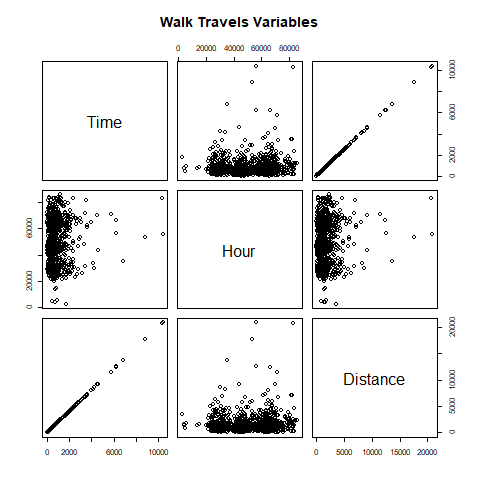
\includegraphics[width=0.8\textwidth]{figuras/chap-sp/scatter_walk.png}
\caption{Correlation among Pedestrian travels variables}
\label{fig:scatter_walk}
\end{figure}

Our pedestrian model is simple, but it is possible to extend it adding information about the pedestrian such as age and mobility difficulties. We did not find any model in the literature that use personal information to model the pedestrian speed, but the information is available in the origin-destination survey.

\subsubsection{Bus Travels}

The bus travels also suffer the impact of the traffic in the city. Figure \ref{fig:travel_time_bus} shows the mean travel time of the buses ad the total number of arrivals per hour.  In the first graph is possible to verify that the mean travel time of the buses in the peak hour are almost 15\% bigger than the other hours. Also, as showed in the second chart, during the peak hours the number of buses moving in the city is almost the double of the rest of the day.

\begin{figure}[!htb]
\centering
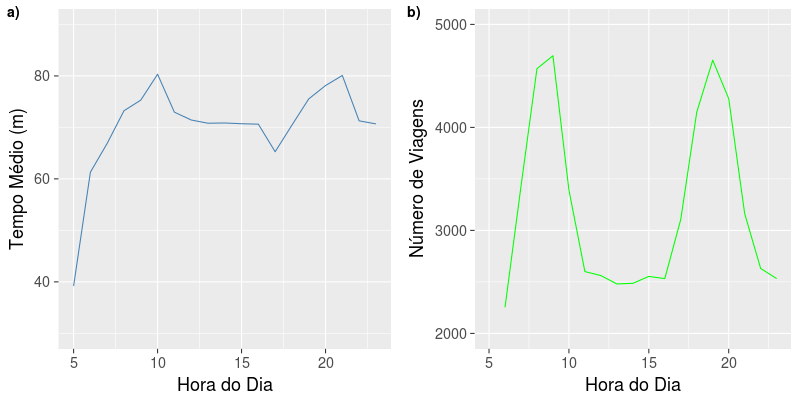
\includegraphics[width=1\textwidth]{figuras/chap-sp/time_distance_bus.png}
\caption{Analyzes of bus travels}
\label{fig:travel_time_bus}
\end{figure}

Regarding the people that travel by bus, Figure \ref{fig:scatter_bus} presents the correlation of time and the hour of the day. The chart shows that exists many long travels with more than 3 hours and the bigger trips are during the morning peak and in the night starting in the night peak.

\begin{figure}[!htb]
\centering
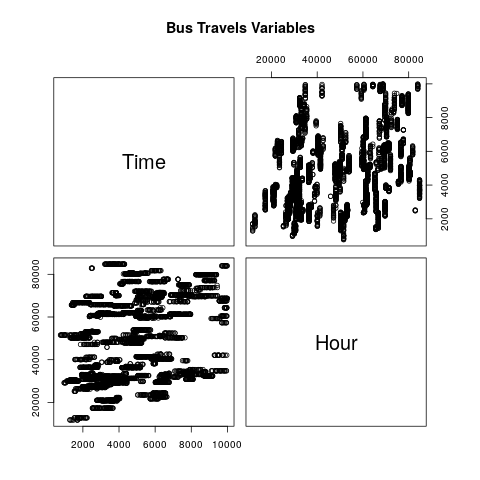
\includegraphics[width=0.8\textwidth]{figuras/chap-sp/scatter_bus.png}
\caption{Correlation among Bus travels variables}
\label{fig:scatter_bus}
\end{figure}

\subsection{Verification}

To verify the models, we compared the real travel time that is in the OD survey with the simulation travel time. This approach has some limitations, for example, most of the answers in the OD are rounded, because typically people approximate their travel time when answering the survey. Another problem is that the OD is from 2012 and we are using the mobility infrastructure of 2018. In the pedestrian and cars travels it will have a limited impact as the streets and roads did not change so much. However, the bus and subway travels are significantly affected by this problem because the city now has new subway lines, and the bus lines are modified continuously.

Figure \ref{fig:box_plot_real_simulated} presents the comparison of all travels. The chart shows that the travel time from simulated and real environments is between 300 and 6000 seconds. The median of the simulated travels are 1800 seconds and of the real travel are 1840 seconds, an error of only 2,5\%. This difference is caused mostly by the buses travels as we will show in the next figures.

\begin{figure}[!htb]
\centering
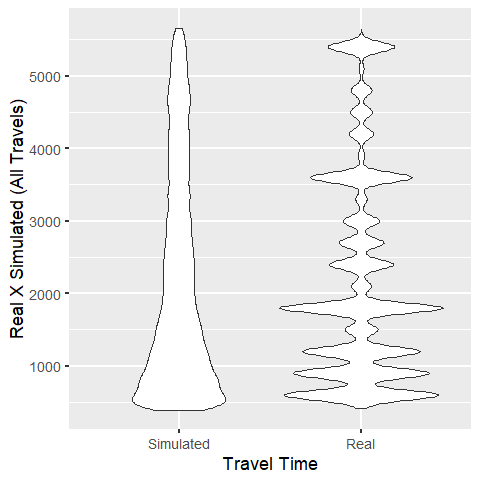
\includegraphics[width=0.5\textwidth]{figuras/chap-sp/total.png}
\caption{Travel time in real and simulated environments}
\label{fig:box_plot_real_simulated}
\end{figure}

Figure \ref{fig:box_plot_real_simulated_bus_subway} presents the comparison of cars and pedestrian travels. Regarding the cars travel, the chart shows that the travel time from simulated and real environments is between 300 and 5000 seconds. The median of the simulated travels is 1655 seconds and of the real travel are 1756 seconds, a difference of 6\%. This difference shows that the mesoscopic model used in the InterSCSimulator is reproducing well the city environment.

Regarding the pedestrian travels, the chart shows that the travel time from simulated and real environments is between 300 and 3000 seconds. The median of the simulated travels are 880 seconds and of the real travel are 868 seconds, a difference of 1\%. This difference shows that the model used in the InterSCSimulator is reproducing well the city environment, mainly because simulating a mesoscopic pedestrian behavior is very straightforward.

Figure \ref{fig:box_plot_real_simulated_bus_subway} presents the comparison of subway and bus travels. Regarding the subway travels, the chart shows that the travel time from simulated and real environments is between 300 and 7000 seconds. The median of the simulated travels are 4080 seconds and of the real travel are 3805 seconds, a difference of 7\%. The subway model is also simple to simulate, most of the difference in this model is caused by the buses that are used by some commuters to arrive at a subway station.

Regarding the bus travels, the chart shows that the travel time from simulated and real environments is between 1000 and 6000 seconds. The median of the simulated travels is 3585 seconds and of the real travel are 3240 seconds, an error of 11\%. This difference shows that the model used in the InterSCSimulator is not reproducing well the city environment. The cause of this difference is that the bus travels are much harder to reproduce for different reasons such as the schedule of the buses varies a lot in S\~ao Paulo, the city has more than 2000 lines, and it is necessary to analyze one by one to reproduce the exact itinerary of the buses. Finally, for commuters that use more than one bus line, it is hard to reproduce their exact itinerary.

A work based on the simulator developed in a Smart City course implemented a much better bus model to the simulator. However, we did not integrate this model with the original models of InterSCSimulator yet. We will present this model in Section \ref{sec:mobiity_model}.

\begin{figure}[!htb]
\centering
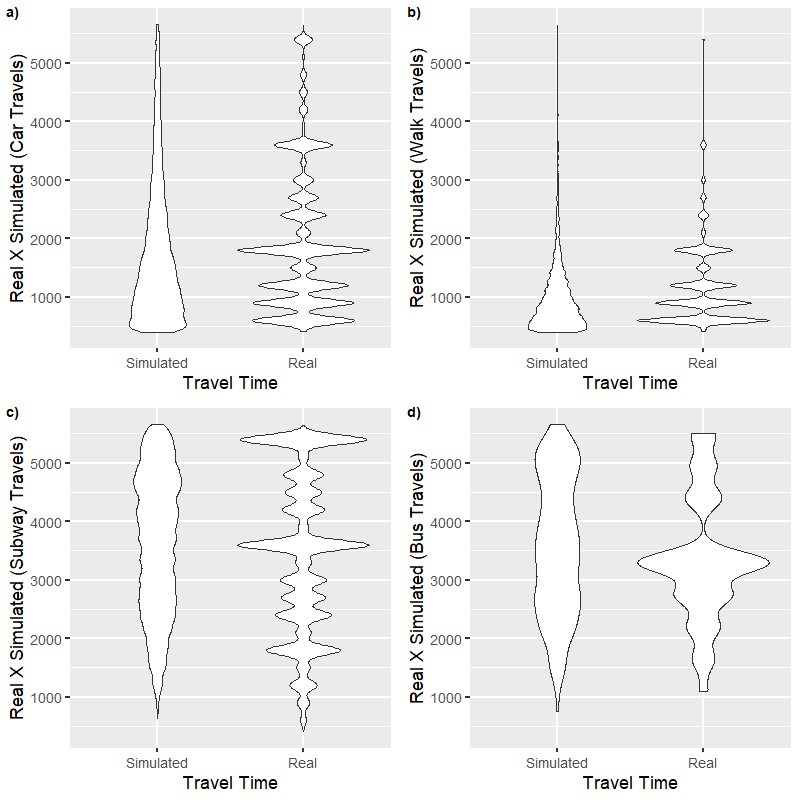
\includegraphics[width=1\textwidth]{figuras/chap-sp/total_modes.png}
\caption{Car, Pedestrian, Subway and Bus Travel time in real and simulated environments}
\label{fig:box_plot_real_simulated_bus_subway}
\end{figure}

\par


\chapter{Scalability Evaluation}
\label{cap:avaliacao}


\section{Vertical Scalability}
\label{sec:vertical_escalabilidade}


\section{Horizontal Scalability}
\label{sec:horizontal_escalabilidade}

\section{Conclusions}
\label{sec:conclusions}
\par

\chapter{Simulator Use Cases}
\label{cap:uses}

This chapter presents the utilization of the InterSCSimulator to support other research during the last two years. Section \ref{sec:test} presents the utilization of the simulator to perform experiments on InterSCity Platform, a Smart City software platform. Section \ref{sec:paraisopolis} describes the simulation of different mobility scenarios in the Paraísopolis community in S\~ao Paulo. Section \ref{sec:vanet} presents the simulation of Vehicular Ah-Doc Networks (VANETs) aided by mobility traces generated from InterSCSimulator. Finally, Section \ref{sec:mobiity_model}

\section{InterSCity Platform Integration}

To test Smart City services and applications, we integrated the InterSCSimulator and InterSCity Platform. The InterSCity platform is an open source micro-services-based platform to enable collaborative research, development, and experiments in smart cities. The platform handles the mandatory requirements to support integrated smart city services and applications in different domains such as transportation, health-care, and environmental monitoring. The integration is performed in two ways:

\begin{itemize}

\item \textbf{Application Request: } The platform simulates the access of a person to a Smart City application deployed in the platform. To simulate it, the simulator makes an HTTP request to a platform service that sends a response with the data requested. The simulator must handle the response and change the behavior of the actor that sends the request.

\item \textbf{City Infrastructure: } The simulator is also capable of simulating city sensors which generate data and send to the platform. This data is sent to the platform using a queue system deployed in the platform.

\end{itemize}

Figure \ref{fig:integration} presents the integration of the platform and the simulator. The application request integration is at the top of the figure, showing that the simulator makes a request and receive a response from the platform. The City Infrastructure integration is at the bottom of the figure, showing that the simulator sends sensor data to the platform.

\begin{figure}[!htb]
\centering
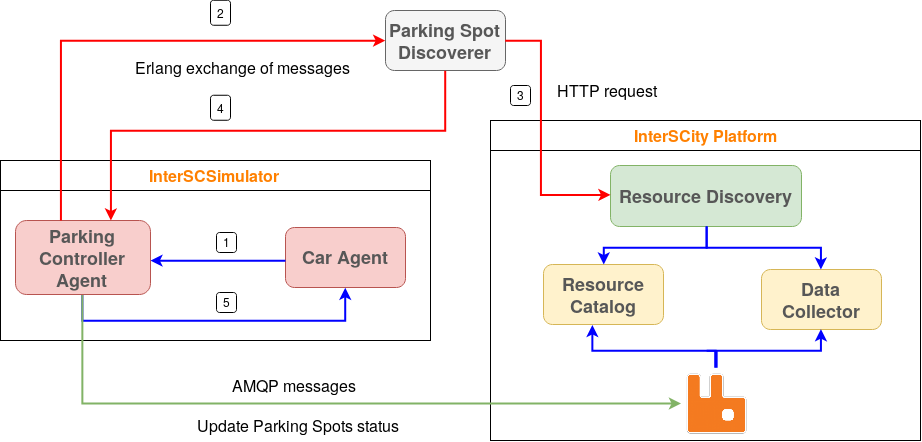
\includegraphics[width=0.8\textwidth]{figuras/chap-uses/integration.png}
\caption{Platform Response Time}
\label{fig:integration}
\end{figure}

The InterSCity research group tested a Smart Parking application using the simulator-platform integration. The scenario was: (1) a driver makes an HTTP request to the platform seeking a parking spot; (2) the platform sends a parking spot and its location; (3) the driver changes its route to go to the parking spot; (4) when the driver stops the car in the parking spots, update the state of the spot sensor in the platform. Steps 1, 2, and 3 are implemented using the application request integration, and step 4 using the city infrastructure integration.

\subsection{InterSCity Platform Scalability Experiments}
\label{sec:test}

The focus of InterSCity platform is to handle the required scalability of a Smart City platform. It is necessary because a Smart City will have thousands of applications and millions of users. The platform has to deal with a considerable variation in the load during the day. For example, a traffic application will be hugely used during the peak hour and normal use in the other hours.

As perform scalability experiments in real environments is not easy, the developers of the platform used the simulator integration to generate a massive workload to the platform. The simulated scenario was the Smart Parking application in the morning peak hour in the city of S\~ao Paulo. The simulation had more than 400 thousand simulated cars, and each car made one or more requests to the platform searching for a parking spot.

Figure \ref{fig:workload_interscity} presents the workload generated in the simulator. The number of requests increase with the passage of time and allow the verification of the behavior of the platform with the variation of the load. The figure presents the workload mean of 15 executions of the platform experiments.

\begin{figure}[!htb]
\centering
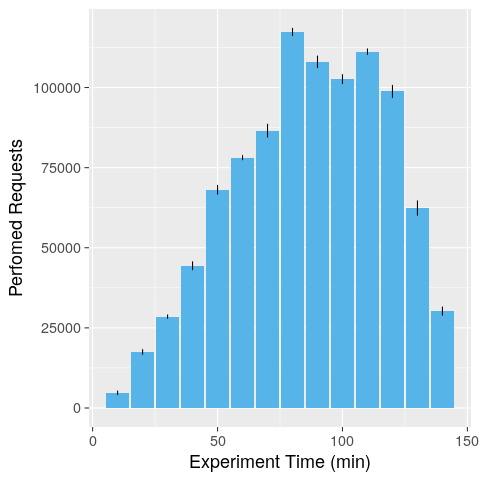
\includegraphics[width=0.6\textwidth]{figuras/chap-uses/load_mean.png}
\caption{Workload generated in the simulation}
\label{fig:workload_interscity}
\end{figure}

The simulator developers executed more than 50 experiments using the simulator, aiding them to find many problems in the platform implementation and achieve the desired scalability. Figure \ref{fig:response_time_interscity} presents the response time of the platform using the load of Figure \ref{fig:workload_interscity}. 

\begin{figure}[!htb]
\centering
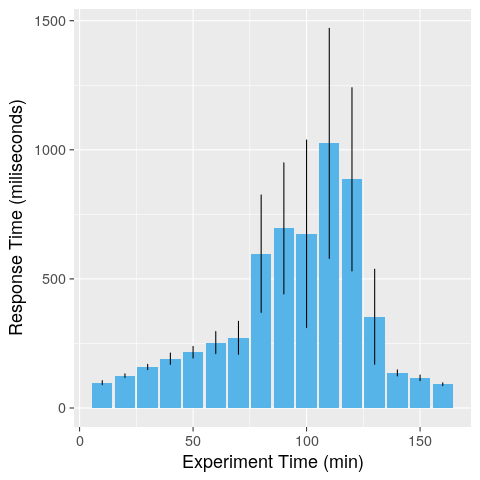
\includegraphics[width=0.6\textwidth]{figuras/chap-uses/response_time_mean.png}
\caption{Platform Response Time}
\label{fig:response_time_interscity}
\end{figure}



\section{Scenarios in Paraisópolis}
\label{sec:paraisopolis}

InterSCSimulator is useful to compare large-scale mobility scenarios. The Traffic Engineering Group from the Polytechnic School from the University of S\~ao Paulo used the simulator to study the impact of a subway line under construction in the city of S\~ao Paulo, especially in the Paraisópilis community, one of the largest poor neighborhoods of the city. This subway line will have two stations in the community, and it will have a significant impact on the population access to quality transportation.

In their work, they examined four simulated scenarios based on a city origin-destination survey and compared their travel time, financial cost, and carbon footprint of the simulated population. They based all the scenarios on realistic changes that might occur with the new subway line. Besides the OD, they also used data from the city buses and metro lines. They simulated the entire community population (approximately 44 thousand people) and other cars from the city to generate car traffic.

The simulation showed that the users of buses could benefit from a decrease in their trip time, and car uses can have economic benefits with the new subway line. For example, of the population that used cars in the original scenario, approximately 1,500 had their travel times decreased, and 4,000 had their travel times increased. The people that had their travel time increased by more than 30 minutes (around 2,000 people) are unlikely to change their travel mode. However, since the cost reduction can be very substantial (mainly when taking into consideration parking fees), even some of them might prefer the subway.

\begin{figure}[!htb]
\centering
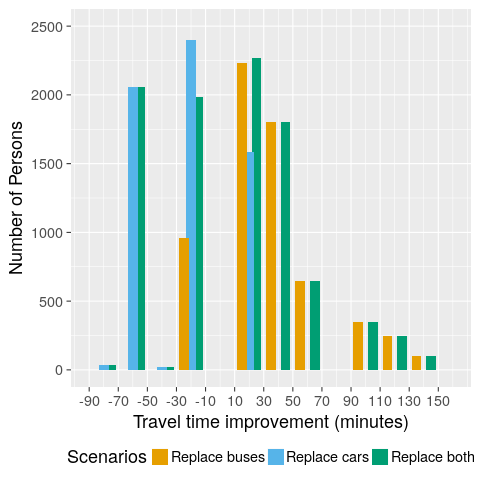
\includegraphics[width=0.6\textwidth]{figuras/chap-uses/hist_travel_time.png}
\caption{Travel time improvement}
\label{fig:travel_time}
\end{figure}

\section{VANETs Simulation}
\label{sec:vanet}

Using the S\~ao Paulo simulation presented in Chapter \ref{cap:sao_paulo} we generated mobility trace to enable tests and experiments of Vehicular Ah-Doc Networks (VANETs). The trace contains the events of all the cars of the simulation during an entire day. The advantage of this trace comparing with other traces available in the literature is the enormous amount of vehicles. While the trace generated in this research contains more than 4 million travels of buses and cars, the other traces contains less than 700 thousand travels.

To show the use of this trace, we converted the output of InterSCSimulator to the input format of NS-3\footnote{NS-3 -- https://www.nsnam.org/}, a popular network simulator. Listing \ref{list:trace_ns3} presents an example of a NS-3 input file.

\renewcommand{\thelstlisting}{\arabic{lstlisting}}
\begin{lstlisting}[caption=NS-3 input file, label=list:trace_ns3, upquote=true]
$node_(0) set X_-23.55084
$node_(0) set Y_-46.62869
$node_(0) set Z_ 0
$ns_ at 15451 "$node_(0) setdest -23.55084 -46.62869 0"
$node_(1) set X_-23.55084
$node_(1) set Y_-46.62869
$node_(1) set Z_ 0
$ns_ at 15469 "$node_(1) setdest -23.55084 -46.62869 0"
\end{lstlisting}

In the file, the lines starting with a \textdollar node, define the creation of network node in the NS-3. The lines starting with \textdollar ns represent the movements of the vehicles and occurs many times until the vehicle arrives at its destination. We used this file in an NS-3 simulation which creates a vehicular network based on the distance of the vehicles. The simulation generates a MAC address to each vehicle, and at each simulation steps it connects or disconnects the vehicles. Listing \ref{list:ns3_output} presents an example of the output of an NS-3 simulation.

\renewcommand{\thelstlisting}{\arabic{lstlisting}}
\begin{lstlisting}[caption=NS-3 Output, label=list:ns3_output, upquote=true]
15469 0 -23.5508 -46.6287 00:00:00:00:00:01 0 
15469 1 -23.5508 -46.6287 00:00:00:00:00:02 0 
15470 0 -23.5508 -46.6287 00:00:00:00:00:01 1 
00:00:00:00:00:02 
15484 2 -23.5508 -46.6287 00:00:00:00:00:03 0 
15485 0 -23.5517 -46.6279 00:00:00:00:00:01 2 
00:00:00:00:00:02 00:00:00:00:00:03 
\end{lstlisting}

Each line in the file corresponds to a vehicle in an instant of the simulation. The attributes are the simulation time, the latitude and longitude, the numbers of cars connected to the vehicle, and the MAC address of all connected cars. From this output files, it is possible to perform different analyses such as the number of connections and disconnections per second and the mean number of connections to the simulated vehicles. For example, Figure \ref{fig:media_conexoes} presents a graph with the mean number of connections per vehicle during 07:00 and 07:02 in the whole city. 

\begin{figure}[!htb]
\centering
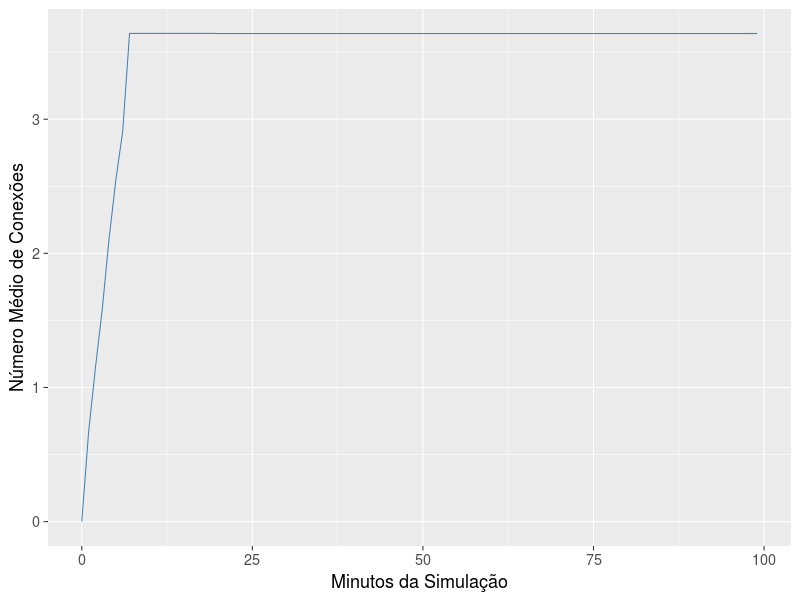
\includegraphics[width=0.6\textwidth]{figuras/chap-uses/num_conexoes.png}
\caption{Mean number of connections during the simulation}
\label{fig:media_conexoes}
\end{figure}

\section{Bus Model Experiments}
\label{sec:mobiity_model}

The InterSCSimulator was used by a study group of a Smart City course to make experiments of a bus mobility model. They created the model based on the real traces of the movement of the buses of S\~ao Paulo provided by the transportation secretariat of the city (SpTrans). The original bus mobility model from InterSCSimulator used the planned intervals to create the buses on the simulation and compared the speed of the buses with the general traffic in the simulation.

However, using the real data from the city, collected by the Automatic Vehicle Location (AVL), the group showed that there are great differences in the planned and real intervals of the city buses. With this data, the group extended the bus mobility model with more accurate data, improving the results of the simulator. Moreover, the students compared the simulated and the real travels times and showed that the results were very close to the real system. Figure \ref{fig:simulation_real_comparison} compares the simulated and the real times.

\begin{figure}[!htb]
\centering
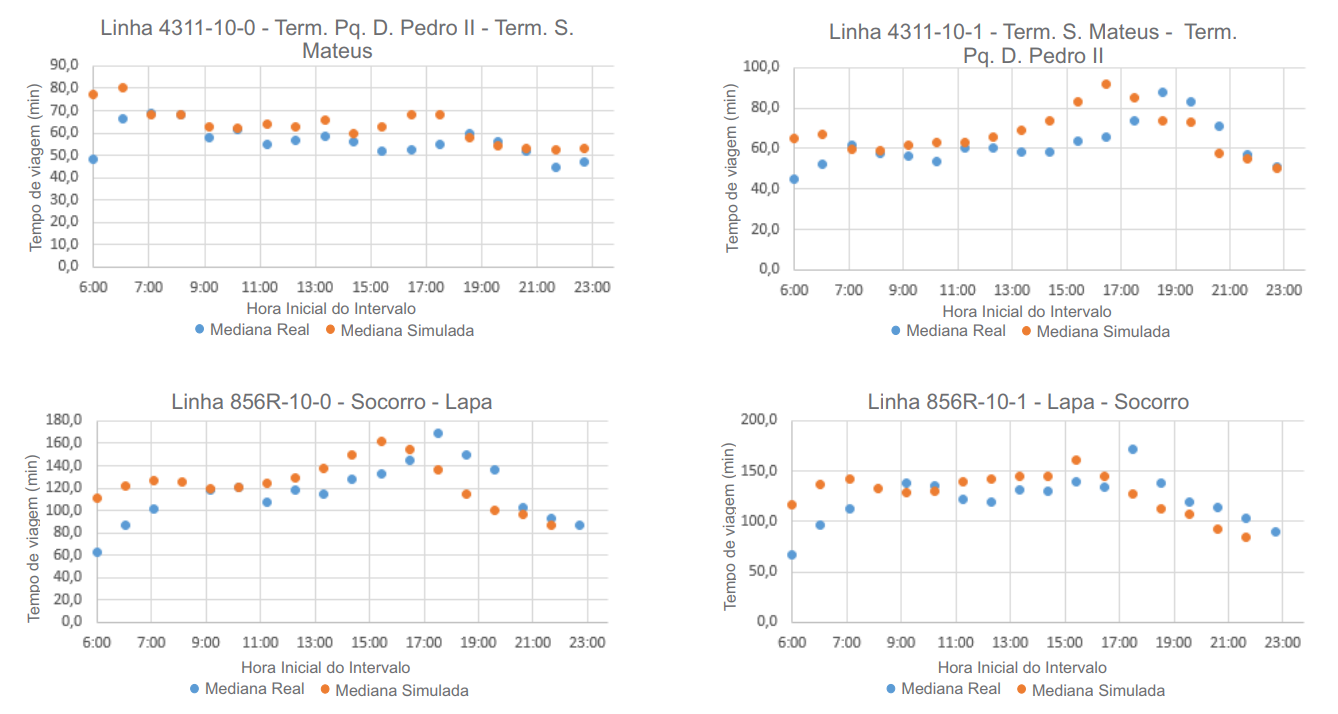
\includegraphics[width=1\textwidth]{figuras/chap-uses/bus_model.png}
\caption{Simulation and Real Time Comparison}
\label{fig:simulation_real_comparison}
\end{figure}

\section{Digital Rails}
\label{sec:digital_rails}

Autonomous vehicles (AVs) technology brings new solutions and challenges for urban mobility. The development and adoption of AVs has the potential to reduce traffic jams and increase traffic safety. However, despite the advancement of automation technology in both research and commercial environments, full autonomous vehicles requiring no human intervention are not expected to be available in the short-term. 

A work investigated the Digital Rails (DR), a proposal to allow AVs to share the roads with regular vehicles, with minimal changes to the current cities infra-structure. DR consists on dedicated lanes for AVs that allows AV platoons to traverse arterial roads at high speeds and synchronized traffic signals coordinates the traffic with regular vehicles. On roads with DR lanes, traffic signals on successive intersections should be synchronized to allow the platoons to travel without stops.The proposal for Digital Rails was first elaborated by designers at a design consultancy firm called Questtonó\footnote{\url{https://www.questtono.com/en/}}. 

The analyses evaluated the impact that such system could have in traffic using simulations based on the city of São Paulo. The DR simulations expanded the InterSCSimulator implementing a couple of features on the simulator such as the synchronized traffic signals, the exclusive AV lanes, and the AV movement model. Figure \ref{fig:dr_network} presents the DR network simulated in the city of S\~ao Paulo.

\begin{figure}[!htb]
\centering
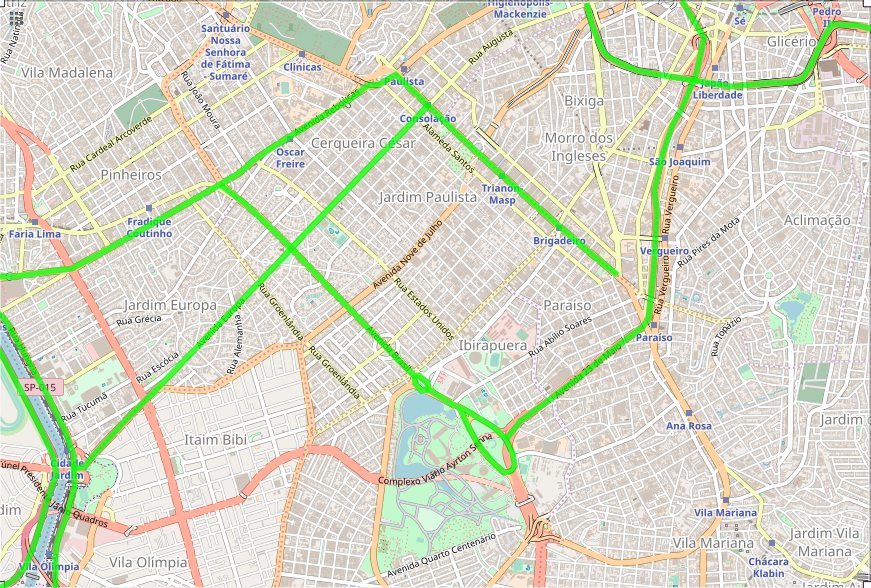
\includegraphics[width=1\textwidth]{figuras/chap-uses/proposal.png}
\caption{DR network simulated in the city of São Paulo}
\label{fig:dr_network}
\end{figure}

To simulate the impact of the DR in the city, it was created a scenario based on the simulation presented in Chapter \ref{cap:sao_paulo}. Four simulations were executed, the first with 0\% of DR vehicles, the second with 25\% and the last with 75\%. As expected, the average travel time increased when the ratio is 0, because the assignment of a lane for DR decreased the road capacity on the selected arterial ways. 
With 25\% of vehicles able to use DR, the average travel time were lower or very similar to the benchmark scenario. For ratios greater than 50\% of vehicles able to use DR, all average times were lower than the benchmark. With 100\% of vehicles able to use DR, the travel times were about 65\% of the benchmark.

We also analyze travel times considering only vehicles that are not able to use DR. Figure \ref{fig:dr-sp-out} shows the evolution of travel times for them. With a ratio of 25\% of vehicles able to use DR, the average travel time is equal or lower than in the benchmark scenario. For ratios higher than 50\%, the average travel time is smaller than in the benchmark scenario. Finally, for 75\% of vehicles able to use DR, the average travel time is between 67\% and 79\% of the benchmark scenario.
\par

\chapter{Conclusions and Future Work}
\label{cap:conclusoes}

Simulators are important tools to develop and evaluate modifications in the city infrastructure and possible public policies. The Smart City community can have a great benefit using simulators, mainly to facilitate experiments and evaluation of city applications, and scientific hypothesis. However, there are many challenges to the effective simulators usage such as scalability, lack of appropriate models, and difficult to use state-of-the-art tools.

This research aimed to provide tools to face some of the challenges of developing a city simulator able to model large-scale scenarios. The main result of this work is the development of InterSCSimulator, a open-source, scalable, Smart City simulator. This simulator is capable of simulating an entire metropolis such as S\~ao Paulo with more than 15 million travels. Moreover, the simulator was already used in many technical and scientific projects as showed in Chapter \ref{cap:uses}.

\section{Contributions}

This work had technical and scientific contributions to the fields of Smart Cities, Large-Scale Simulations, and Software Integration. In the following we summarize the main outcomes of this work:

\subsection{Technical Contributions}

\begin{description}

\item[Smart City Simulator:] We developed the simulator which is available as an open source software to all the Smart City community. The software already implements many traffic models and is extensible to new city scenarios allowing city planning and test of scientific projects.

\item[Large-Scale Experiments:] We conducted scalability experiments to evaluate the maximum load of the InterSCSimulator using the Google Compute Engine in the cloud. Our tests showed that the simulator is capable of running in large-scale machines with more than 64 CPUs and 300 GBs of memory.

\item[Smart City Platform and Simulator Integration:] The InterSCity platform and the InterSCSimulator are already integrated. Thus, it is possible to develop and test new applications on the platform using the simulated data and also validate new simulations scenarios with the data stored in the platform.

\end{description}

\subsection{Scientific Contributions}

\begin{description}

\item[Smart City Simulator Scalability:] We demonstrated the scalability of the simulator through experiments that started with 10\% and finished with 100\% of the population of S\~ao Paulo simulated.

\item[Experiments Using the Simulator:] We showed different works that used the simulation to evaluate their proposals such as the Digital Rails autonomous vehicles, the S\~ao Paulo bus movement model, and the scalability experiments of the InterSCity platform.
 
\end{description}

\subsection{Educational Contributions}

\begin{description}

\item[Courses: ] The simulator was used in a Smart City course to support the tests of a new bus traffic model in the city of S\~ao Paulo. The model is based on real data collected from the city buses.

\item[Capstone Project: ] An undergraduate student used the simulator to develop a simulation of Digital Rails, a new transportation mode that uses autonomic vehicles and semaphore synchronization. The project extended the simulator to allow the simulation of this new transportation approach.

\item[Master Thesis: ] InterSCSimulator supported the development of two master thesis. The first, allowing the realistic, large-scale experiments to analyze the scalability of InterSCity platform. The second, the simulator was used as study-case to an approach to integrate Smart Cities simulators and platforms to allow tests and experiments in Smart Cities platforms, services, and applications.

\item[Educational Material:] The material produced from the bibliographic review of Smart Cities was used to at least three Smart Cities courses in universities in Brazil and in computer science conferences.

\end{description}






\section{Publications}
\label{sec:publicacoes}

Based on the research presented in this thesis, we published seveb scientific papers or book chapters. Three regarding the literature review, two about InterSCSimulator architecture, and two showing the use of the simulator. The complete list of publications are in the following:

Santana, E.F.Z., Chaves, A.P., Gerosa, M.A., Kon, F. and Milojicic, D. Software platforms for smart cities: Concepts, requirements, challenges, and a unified reference architecture. ACM Computing Surveys (CSUR) 50.6 (2017): 78.

Kon, F.; Santana, E. F. Z. Cidades Inteligentes: Tecnologias, Aplicações, Iniciativas e Desafios. In: José Carlos Maldonado; José Viterbo; Marcio Eduardo Delamaro; Sabrina Marczak. (Org.). Jornadas de Atualização em Informática. 1 ed.Porto Alegre: Sociedade Brasileira de Computação, 2016.

Kon, F.; Santana, E. F. Z. Computação aplicada a Cidades Inteligentes: Como dados, serviços e aplicações podem melhorar a qualidade de vida nas cidades. In: Flávia Delicato; Paulo Pires. (Org.). Jornadas de Atualização em Informática. 1 ed. Porto Alegre: Sociedade Brasileira de Computação, 2017.

Santana, E. F. Z., Bastista, D. M., Kon, F. and Milojicic, D. S. SCSimulator: An Open Source, Scalable Smart City Simulator. In Tools Session of the 34th Brazilian Symposium on Computer Networks (SBRC). Salvador, Brazil, 2016.

Santana, E. F. Z.; Lago, N. ; KON, F. ; Milojicic, D. InterSCSimulator: Large-Scale Traffic Simulation in Smart Cities using Erlang. In 18th Workshop on Multi-agent-based Simulation (MABS), São Paulo, Brazil, 2017.

Santana, E. F. Z., Kanashiro, L., Tomasiello, D., Kon, F., Giannotti, M. "Analyzing Urban Mobility Carbon Footprint with Large-scale, Agent-based Simulation." SMARTGREENS. 2018.

Santana, E. F. Z., Kanashiro, L., Kon, F. Geração de Rastros de Mobilidade para Experimentos em Redes Veiculares. II Workshop de Computação Urbana (CoUrb). 2018.

Besides, two other papers were published using the InterSCSimulator as support tool.


\section{Future Work}

There are several future work regarding the InterSCSimulator such as improvements in the simulator implementation including new features and changes in its architecture and the inclusion of new Smart Cities scenarios. Regarding the improvements in the simulator implementation:

\begin{description}

\item[Distributed Simulations:] The current version of InterSCSimulator does not allow distributed simulations, mainly because of the use of ETS tables that are not distributed across a Erlang network. Therefore, to distribute the InterSCSimulator it will be necessary to implement a synchronization service that updates the ETS table in all Erlang nodes that are executing the simulator.

\item[Real-Time Visualization:] The tool that we are using to visualize the simulations only work with the entire log of simulation already generated. We plan to develop a tool that can get the data directly from the simulator and generate an animated visualization  of the simulation.

\item[Simulation of Events:] We intend to add the occurrence of events in the city that can change the traffic behavior such as rain, accidents, and road closures.

\item[Real-Time Integration with a Network Simulator:] 

\end{description}

Regarding the new Smart Cities scenarios:

\begin{description}

\item[Waste Management:] It is possible to simulate the waste trucks and the city infrastructure to the waste management system such as trash disposals and trash bins. With this scenario is possible to measure the efficiency of the system and test algorithms to create the routes to the trucks.

\item[Health-Care:] The InterSCSimulator already allows the simulation of buildings that can be the origin or the destination of travels. Using this idea, it is possible to simulate hospitals that are the destination of people with health problems. Using this scenarios is possible to analyze the time that the city inhabitants are taking to go to a hospital and measure the necessity of medical units in different regions of the city.

\end{description}
\par
\par


%%%%%%%%%%%%%%%%%%%%%%%%%%%%%% SEÇÕES FINAIS %%%%%%%%%%%%%%%%%%%%%%%%%%%%%%%%%%%

% Aqui vão a bibliografia, índice remissivo e outras seções similares.
% O comando backmatter desabilita a numeração de capítulos e também não existe
% na classe "article".
\backmatter

% Este formato está definido na package imeusp-headers
\pagestyle{frontback}

% A bibliografia é obrigatória

%%%%%%%%% Bibliografia com natbib (preterido): %%%%%%%%%
%\bibliographystyle{extras/alpha-ime}% citação bibliográfica alpha
%\bibliographystyle{extras/plainnat-ime} % citação bibliográfica textual
%\bibliography{bibliografia}  % associado ao arquivo: 'bibliografia.bib'

%%%%%%%% Bibliografia com biblatex (preferido): %%%%%%%%

\printbibliography[
  title=\refname\label{bibliografia}, % "Referências", recomendado pela ABNT
  %title=\bibname\label{bibliografia}, % "Bibliografia"
  % Inclui a bibliografia no sumário; comente se estiver usando "article"
  heading=bibintoc,
]

\end{document}
